  \documentclass[b5paper,11pt,fleqn,openright]{memoir}
\semiisopage[12]
\setlength{\uppermargin}{60pt}
\setlength{\headsep}{24pt}
\checkandfixthelayout[nearest]

%\usepackage{cmbright}  % nice font

\usepackage[utf8]{inputenc}
\usepackage[T1]{fontenc}      % Add this line
\usepackage[english]{babel}

%\usepackage{lmodern}
%\usepackage{newpxtext}
%\usepackage{antt}
%\usepackage{mathpazo}
%\usepackage{eulervm}
%\usepackage{fourier}
%\usepackage{pxfonts}

\usepackage{kpfonts}%  for math    
\usepackage{indentfirst}

%\usepackage{times}
%\renewcommand{\rmdefault}{lmr} % Set Latin Modern Roman as the default font

\usepackage[hidelinks]{hyperref}
\usepackage{amsmath,amsfonts,amssymb,bm}%,amsthm}
\usepackage{gensymb}
\usepackage[capitalise]{cleveref}
\usepackage{graphicx,subcaption}
\usepackage{siunitx}
\usepackage{stmaryrd}
\usepackage{pgffor}
\usepackage{enumitem}
%\includeonly{mainmatter/uasstop.tex}
\usepackage[final]{pdfpages}

\usepackage{nomencl}
\makenomenclature

%float barrier
\usepackage{placeins}

\usepackage{algorithm}
\usepackage{algpseudocode}

% math stuff
\usepackage{cancel} 
\usepackage{bm}
\usepackage{upgreek}
\usepackage{amsmath}
\usepackage{amssymb}
\usepackage{relsize}
\usepackage{amssymb}

\usepackage{empheq}
\newcommand*\widefbox[1]{\fbox{\hspace{2em}#1\hspace{2em}}}
%pgf plot

\usepackage{pgfplots}
\pgfplotsset{compat=newest}
\usepackage{tikz}
\usetikzlibrary{plotmarks}
\usetikzlibrary{arrows.meta}
\usetikzlibrary{patterns}
\usetikzlibrary{patterns.meta} 
\usetikzlibrary{positioning}

\usepgfplotslibrary{patchplots}

\usetikzlibrary{external}
% \tikzexternalize % activate!
% \usetikzlibrary{shapes.geometric, arrows,positioning, calc, arrows.meta,scopes}
% and optionally (as of Pgfplots 1.3):

\pgfplotsset{plot coordinates/math parser=false}
\newlength\figureheight
\newlength\figurewidth 


\usepackage{multirow}
\usepackage{graphicx}
\usepackage{xcolor}

\usepgfplotslibrary{groupplots, external}

\definecolor{mycolor1}{rgb}{0.00000,0.44700,0.74100}%
\definecolor{mycolor2}{rgb}{0.85000,0.32500,0.09800}%
\definecolor{mycolor3}{rgb}{0.92900,0.69400,0.12500}%
\definecolor{mycolor4}{rgb}{0.46670,0.67450,0.18820}%
\definecolor{mycolor5}{rgb}{0.49400,0.18400,0.55600}%

\newlength{\twosubht}
\newsavebox{\twosubbox}


% definitions
\newcommand{\uniform}{$SG_U$}
\newcommand{\princ}{$SG_P$}
\newcommand{\userdefine}{$SG_A$}

\newcommand{\uniforms}{$SG_U$ }
\newcommand{\princs}{$SG_P$ }
\newcommand{\userdefines}{$SG_A$ }
\renewcommand{\d}{\mathop{}\!\text{d}}
\newcommand{\secref}[1]{Sec.~\ref{#1}}
\newcommand{\chapref}[1]{Chap.~\ref{#1}}
\newcommand{\figref}[1]{Fig.~\ref{#1}}
\renewcommand{\eqref}[1]{Eq.~\ref{#1}}
\newcommand{\tabref}[1]{Tab.~\ref{#1}}
\newcommand{\appref}[1]{App.~\ref{#1}}

\newlength{\imwidth}
\setlength{\imwidth}{14.cm}

\newlength{\imwidthmax}
\setlength{\imwidthmax}{15.cm}

%style=numeric-comp
\usepackage[natbib=true, style=numeric-comp, backend=biber, defernumbers, maxbibnames=99, maxcitenames=2, sorting=none, eprint=false, giveninits=true]{biblatex}
\addbibresource{ownPub/myownpubs.bib}
\addbibresource{bib.bib} 
\AtEveryBibitem{%
  % \clearfield{issn} % Remove issn
  \ifentrytype{online}{}{% Remove url except for @online
    \clearfield{url}
  }
}
\setlength\bibitemsep{1.5\itemsep}



% \definecolor{mylinkcolor}{rgb}{0.6745098039, 0.4196078431, 0.5921568627}%
\definecolor{mylinkcolor}{rgb}{0.,0.5019607843,0.6745098039}%
\definecolor{mycitecolor}{rgb}{0.9294117647, 0.4274509804, 0.4509803922}%
\definecolor{myurlcolor}{rgb}{0.4156862745, 0.6509803922, 0.6862745098}%


\hypersetup{
  linkcolor  = mylinkcolor,
  citecolor  = mylinkcolor,
  urlcolor   = mylinkcolor,
  colorlinks = true,
}



\DeclareFieldFormat{labelnumberwidth}{\mkbibbrackets{#1}}
\renewbibmacro*{cite}{%
  \printtext[bibhyperref]{%
    \printfield{labelprefix}%
    \ifkeyword{myPapers}
      {\printfield{labelnumber}}
      {\ifkeyword{myPapers2}
      {\printfield{labelnumber}}
      {\printfield{labelalpha}%
      \printfield{extraalpha}}}}}



\defbibenvironment{bibliographyNUM}
  {\list
     {\printtext[labelnumberwidth]{%
        \printfield{labelprefix}%
        \printfield{labelnumber}}}
     {\setlength{\labelwidth}{\labelnumberwidth}%
      \setlength{\leftmargin}{\labelwidth}%
      \setlength{\labelsep}{\biblabelsep}%
      \addtolength{\leftmargin}{\labelsep}%
      \setlength{\itemsep}{\bibitemsep}%
      \setlength{\parsep}{\bibparsep}}%
      \renewcommand*{\makelabel}[1]{\hss##1}}
  {\endlist}
  {\item}

\renewbibmacro{in:}{%
  \ifentrytype{article}{}{%
  \printtext{\bibstring{in}\intitlepunct}}}
  
 \preto\fullcite{\AtNextCite{\defcounter{maxnames}{99}}}
  
\newlength\drop
\makeatletter
\newcommand*\titleM{\begingroup% Misericords, T&H p 153
\setlength\drop{0.08\textheight}
\centering
\vspace*{\drop}
{\Huge\mdseries \thetitle }\\[\baselineskip]
%{\scshape the subtitle}\\[\baselineskip]
\vfill
{\large\mdseries \theauthor}\par
\vfill
{\mdseries Department of Civil and Mechanical Engineering\\Technical University of Denmark, 2800 Kongens Lyngby\\\@date}\par
\vspace*{0\drop}
\endgroup}
\makeatother


%\newcommand{\diff}[2]{\frac{\partial #1}{\partial #2}}
%\DeclareMathAlphabet{\mathpzc}{OT1}{pzc}{m}{it}
%\usepackage{mathalpha}

%\DeclareFontFamily{U}{mathx}{\hyphenchar\font45}
%\DeclareFontShape{U}{mathx}{m}{n}{<-> mathx10}{}
%\DeclareSymbolFont{mathx}{U}{mathx}{m}{n}
%\DeclareMathAccent{\widebar}{0}{mathx}{"73}

%\chapterstyle{southall}


\makechapterstyle{southall-mod}{%
  \chapterstyle{default}
  \setlength{\afterchapskip}{1\baselineskip} %%%%%%%%% MOD: WAS 5\baselineskip
  \setlength{\beforechapskip}{18pt}%    \headindent %%%%%%% MOD: WAS 36pt
  \setlength{\midchapskip}{\textwidth}% \rightblock
  \addtolength{\midchapskip}{-\beforechapskip}
  \renewcommand*{\chapterheadstart}{}%\vspace*{0pt}} %%%% MOD: WAS 2\baselineskip
%%%  \renewcommand*{\chaptitlefont}{\huge\rmfamily\raggedright}
  \renewcommand*{\chaptitlefont}{\huge\rmfamily\memRTLraggedright}
  \renewcommand*{\chapnumfont}{\chaptitlefont}
  \renewcommand*{\printchaptername}{}
  \renewcommand*{\chapternamenum}{}
  \renewcommand*{\afterchapternum}{}
  \renewcommand*{\printchapternum}{%
    \begin{minipage}[t][\baselineskip][b]{\beforechapskip}
      {\vspace{0pt}\chapnumfont%%%\figureversion{lining}
                   \thechapter}
    \end{minipage}}
  \renewcommand*{\printchaptertitle}[1]{%
    \hfill\begin{minipage}[t]{\midchapskip}
      {\vspace{0pt}\chaptitlefont ##1\par}\end{minipage}}
  \renewcommand*{\afterchaptertitle}{%
    \par\vspace{\baselineskip}%
    \hrulefill \par\nobreak\noindent \vskip \afterchapskip}}

\newcommand{\InsertBlankPages}[1]{
  \foreach \blank in {1,...,#1} {
    \newpage
    \thispagestyle{plain}
    \mbox{}
  }%
}

\newlength{\commalabelwd}
\newcommand{\commalabel}[2]{%
  \settowidth\commalabelwd{\normalfont#2\hspace{\labelsep}}%
  \normalfont#2\ifdim#1<\commalabelwd\fi\hfill
}

\setlength{\parskip}{1em}

% \chapterstyle{southall-mod}
% \chapterstyle{brotherton}
% \chapterstyle{madsen}
\chapterstyle{veelo}

\setcounter{tocdepth}{3}
\setsecnumdepth{subsection}


\title{Multiphysics topology optimization in nanophotonics}
\author{Beñat Martinez de Aguirre Jokisch}
\date{July 2025}

\newcommand{\red}[1]{{\color{red}#1}}


\begin{document}


\frontmatter

\includepdf[pages=-,width=\paperwidth, templatesize={\paperwidth}{250mm}, offset=0 -0.2mm]{Cover/Front.pdf}
\cleardoublepage


\openany
\begin{titlingpage}
  \titleM
  \clearpage
  \noindent\textbf{Thesis title:} \\\noindent Thesis title
  \vspace{1.5em}

  \noindent\textbf{Author:}\\\noindent Ph.D. Candidate\\Department of Civil and Mechanical Engineering\\ Technical University of Denmark
  \vspace{0.5em}

  \noindent\textbf{Main Supervisor:}\\\noindent Main superviser\\Department of Civil and Mechanical Engineering\\ Technical University of Denmark
  \vspace{0.5em}

  \noindent\textbf{Co-supervisors:}\\
  \noindent Co-superviser\\Department of Civil and Mechanical Engineering\\ Technical University of Denmark
  \vspace{0.5em}

  \noindent\textbf{Funding and competing interests:}\\\noindent This work was funded by the Villum Foundation, through the Villum investigator project InnoTop. The author has no competing interests.
  \vspace{1.5em}

  \noindent\textbf{Duration:}\\\noindent The work has been carried out between the DATA0 and the DATA1.
  \vspace{2.2em}

  \noindent \copyright Ph.D. Candidate
  \vspace{1em}

  \noindent Department of Civil and Mechanical Engineering\\Technical University of Denmark\\ Nils Koppels Allé, Building 404 \\ DK-2800 Kongens Lyngby, Denmark
  \vspace{1em}

  \noindent MEK-PHD ISSN: \#\#\#\#-\#\#\#\#
\end{titlingpage}
\setcounter{page}{3}
\chapter*{Preface}

Bla bla bla...

\noindent Kongens Lyngby, \today,\\
\vspace{0.1cm}\\
\noindent \textit{Ph.D. Candidate}

\chapter*{Abstract}

Bla bla bla...

\chapter*{Resumé}

Bla bla bla...

\cleardoublepage
\chapter*{List of Publications}
\nocite{ownpub0,ownpub1}
\newrefcontext[sorting=none,labelprefix=P]
\printbibliography[env=bibliographyNUM,keyword=myPub,title={List of publications},heading=none,resetnumbers]
\newrefcontext[sorting=none,labelprefix=M]
\printbibliography[env=bibliographyNUM,keyword=myMan,heading=none,resetnumbers]
%https://tex.stackexchange.com/questions/553753/how-to-add-list-of-publication-in-thesis-class
%\endrefcontext

\cleardoublepage

{
  \hypersetup{linkcolor=black}
  \tableofcontents*
}



\mainmatter
\openright
\chapter{Introduction}

Bla bla bla...

Current state-of-the-art design approaches for photonic devices often rely on trial-and-error
experience-based multi-stage approaches using simplified physics models for individual
components. This may in part be due to the extensively developed and well-understood models
for the temporal and spatial confinement of light in pure photonic structures, such as photonic
crystals and waveguides, and in part due to the complexity of the full physics problems. Further, such design approaches often ignore multi-physics effects, such as . If these
effects are strong, and simultaneously have a large influence on the optical field, their omission in
the design process may lead to a suboptimal final device.

This Ph.D. project aims to address these challenges by employing novel
multi-physics design optimization techniques, which accurately capture 
the important effects of the full physics problem.

%\begin{figure}[tb]
%    \centering
%    \makebox[\textwidth][c]{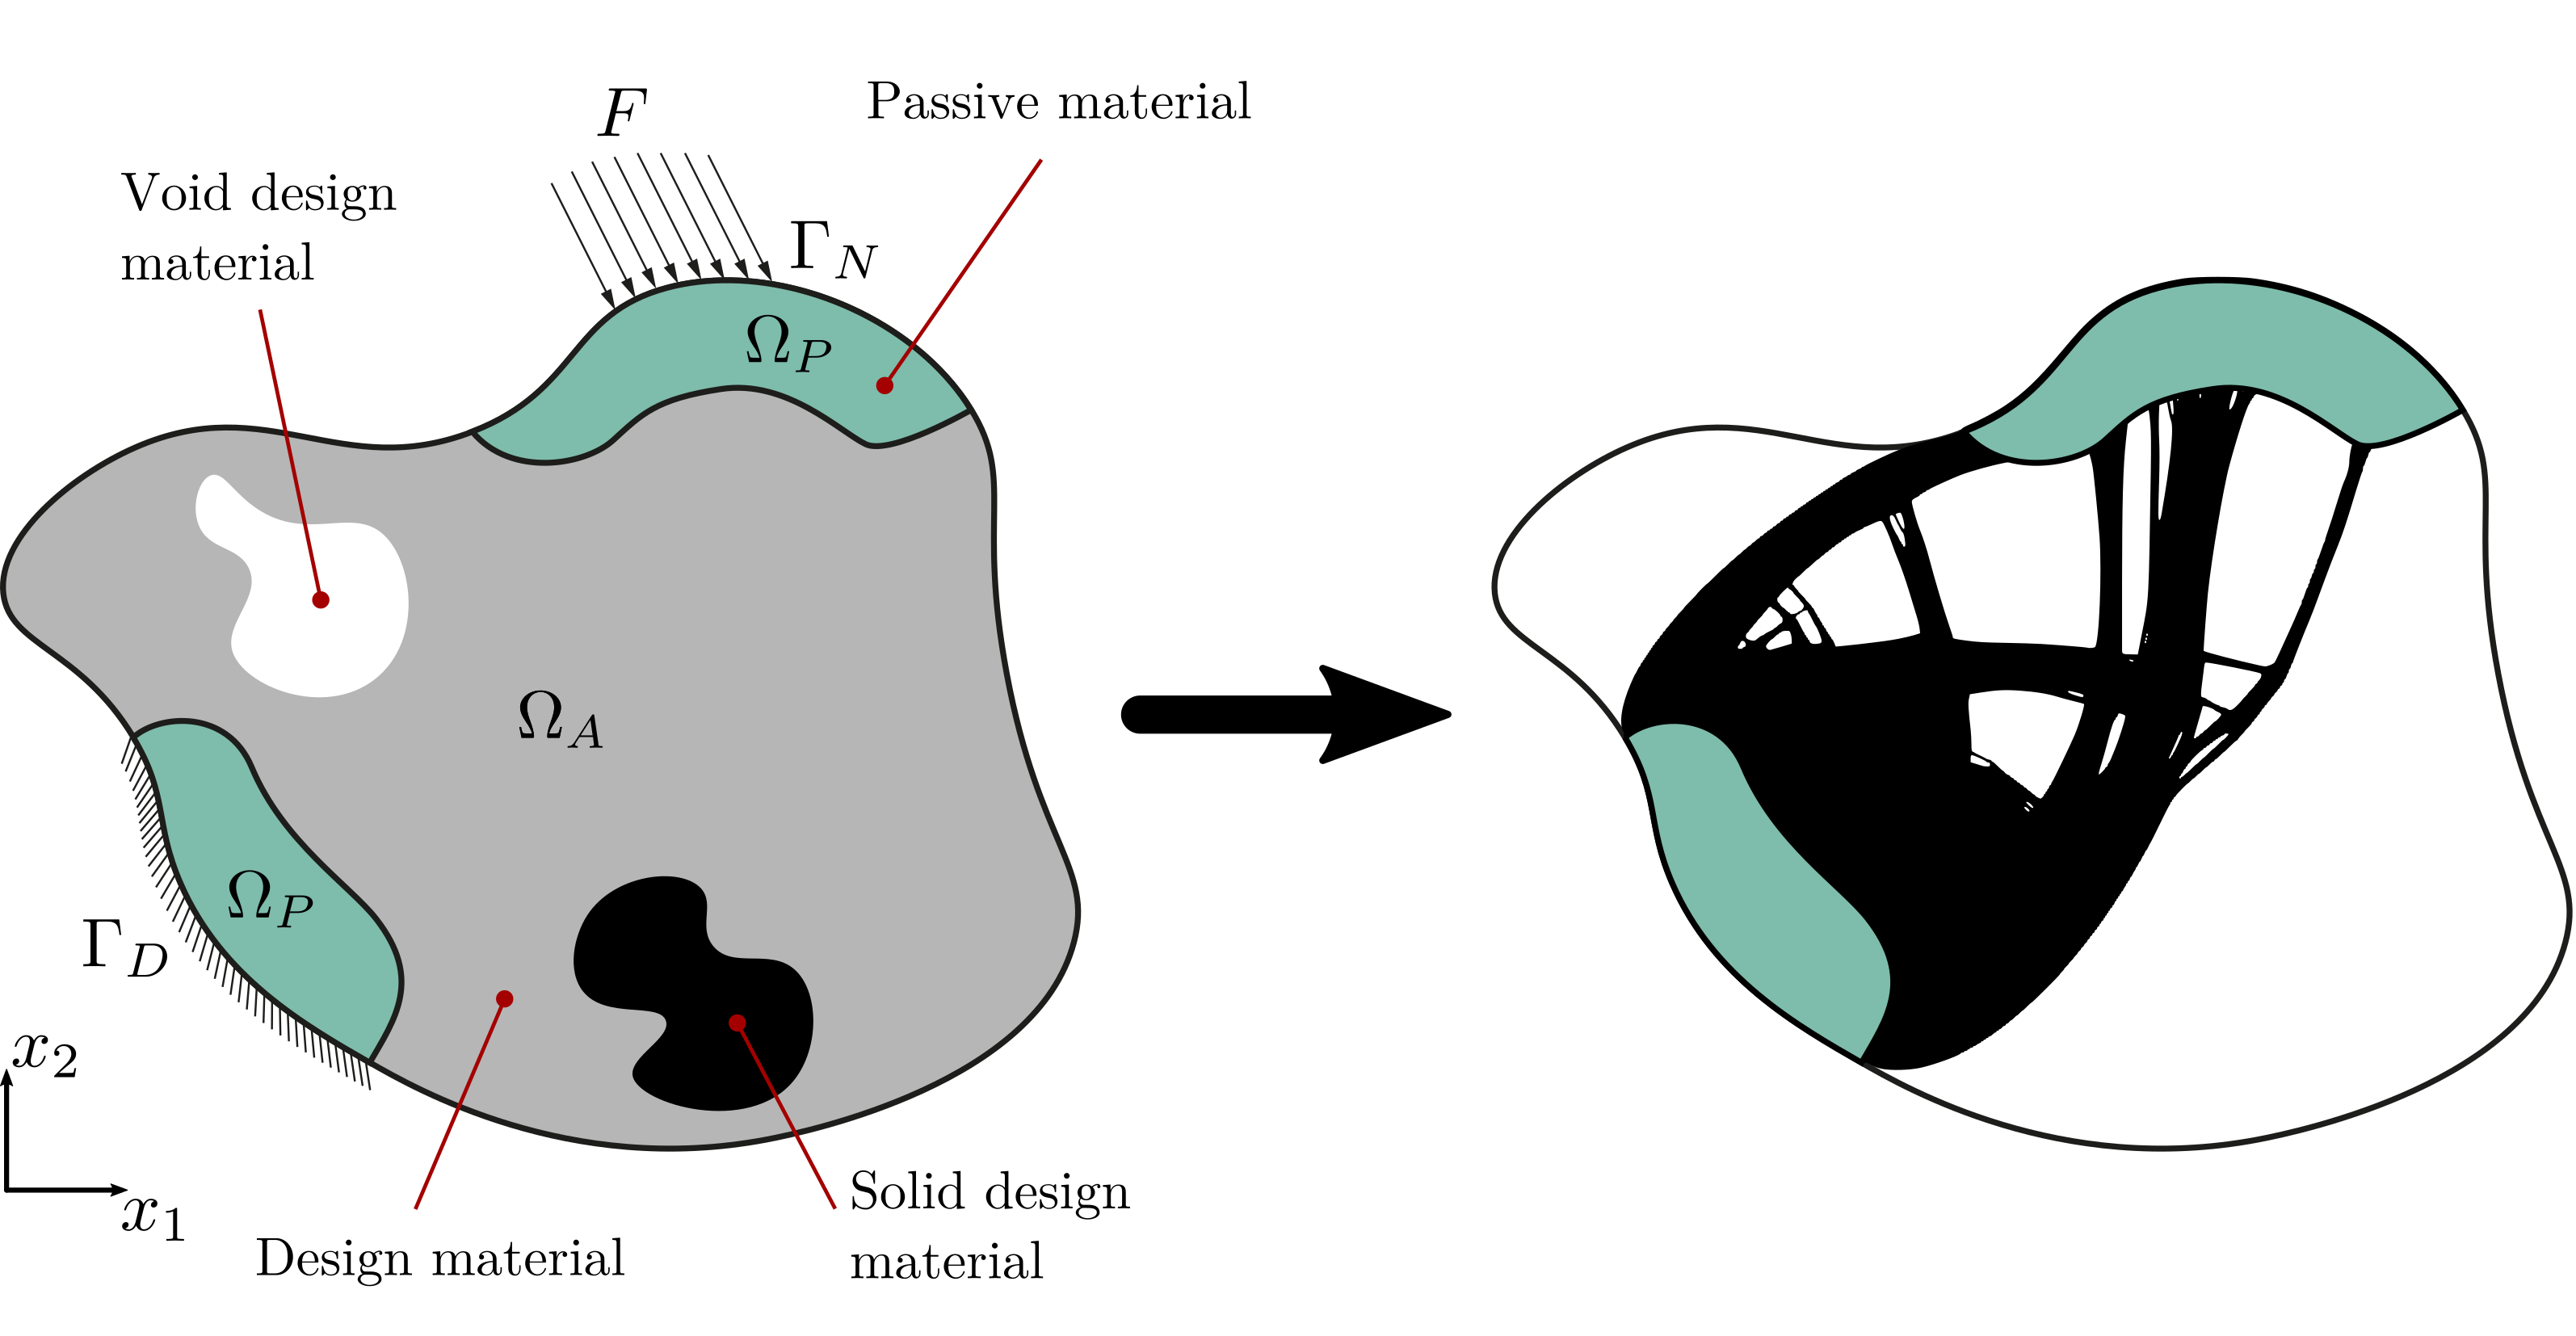
\includegraphics[width=1\imwidth]{figures/simpModel.png}}%
%    \caption{Bla bla bla...}
%    \label{fig:illustateTopOpt}
%\end{figure}


%\begin{equation}
%    (EIu'')'' = q
%\end{equation}


%\begin{figure}[tb]
%    \centering
%    \makebox[\textwidth][c]{\begin{tikzpicture}[remember picture]
    \begin{scope}[xshift=0mm]
        % angle (deg)
        \newcommand\ai{10}
        % line width
        \newcommand\wi{1pt}
        % cell size
        \newcommand\cellsize{3}
        % Rank-$N$ size
        \newcommand\di{0.75}

        % cell
        \draw[gray!10,   fill=gray!10, rotate around={\ai:(0,0)}] (0,0) rectangle (\cellsize,\cellsize) node (rect1) {};
        \draw[black!60, fill=black!60, rotate around={\ai:(0,0)}] (0,0) rectangle (\di,\cellsize);

        % orientation frame
        \draw[black, -stealth, line width=\wi, rotate around={\ai:({\di*cos(\ai) - \cellsize/2*sin(\ai)},{\di*sin(\ai) + \cellsize/2*cos(\ai)})}] ({\di*cos(\ai) - \cellsize/2*sin(\ai)},{\di*sin(\ai) + \cellsize/2*cos(\ai)}) -- ({\di*cos(\ai) - \cellsize/2*sin(\ai) + 0.75},{\di*sin(\ai) + \cellsize/2*cos(\ai)});
        \draw[black, -stealth, line width=\wi, rotate around={\ai:({\di*cos(\ai) - \cellsize/2*sin(\ai)},{\di*sin(\ai) + \cellsize/2*cos(\ai)})}] ({\di*cos(\ai) - \cellsize/2*sin(\ai)},{\di*sin(\ai) + \cellsize/2*cos(\ai)}) -- ({\di*cos(\ai) - \cellsize/2*sin(\ai)},{\di*sin(\ai) + \cellsize/2*cos(\ai) + 0.75});

        % local frame
        \draw[black, -stealth, dashed, line width=\wi] (0,0) -- ({\cellsize + 0.8},0);
        \draw[black, -stealth, dashed, line width=\wi] (0,0) -- (0,{\cellsize + 0.8});

        % ruler
        \draw[black, |-|, line width=\wi, rotate around={\ai:(0,0)}] (0,0) -- (\cellsize,0);
        \draw[black,  -|, line width=\wi, rotate around={\ai:(0,0)}] (0,0) -- (\di,0);

        % arc
        \draw[black, dotted, line width=\wi] (\cellsize,0) arc (0:\ai:\cellsize);

        % annotation
        \draw (\cellsize + 0.7, -0.3) node {$x_1 / \epsilon^3$};
        \draw (-0.5, \cellsize + 0.8) node {$x_2 / \epsilon^3$};
        \draw (\cellsize/2,-0.75) node {Rank-$1$};

        \draw[rotate around={{\ai/2}:(0,0)}] ({\cellsize+0.3},0) node {$\theta_1$};

        \draw[rotate around={{\ai}:(0,0)}] ({\di/2},0.4) node [rotate around={{\ai}:(0,0)}] {$\mu_1$};
        \draw[rotate around={{\ai}:(0,0)}] ({(\cellsize - \di)/2 + \di},0.4) node [rotate around={{\ai}:(0,0)}] {$1-\mu_1$};

        \draw[rotate around={{\ai}:(0,0)}] ({0+0.4},{\cellsize-0.4}) node [rotate around={{\ai}:(0,0)}] {$(+)$};
        \draw[rotate around={{\ai}:(0,0)}] ({\cellsize-0.4},{\cellsize-0.4}) node [rotate around={{\ai}:(0,0)}] {$(-)$};
        \coordinate (A) at (rect1.north);


        \draw[rotate around={\ai:({\di*cos(\ai) - \cellsize/2*sin(\ai)},{\di*sin(\ai) + \cellsize/2*cos(\ai)})}] ({\di*cos(\ai) - \cellsize/2*sin(\ai)+1} , {\di*sin(\ai) + \cellsize/2*cos(\ai) + 0.2}) node {$\mathbf{n}_1$};
        \draw[rotate around={\ai:({\di*cos(\ai) - \cellsize/2*sin(\ai)},{\di*sin(\ai) + \cellsize/2*cos(\ai)})}] ({\di*cos(\ai) - \cellsize/2*sin(\ai) + 0.3} , {\di*sin(\ai) + \cellsize/2*cos(\ai) + 1}) node {$\mathbf{m}_1$};



    \end{scope}
    \begin{scope}[xshift=45mm]
        % angle (deg)
        \newcommand\ai{15}
        % line width
        \newcommand\wi{1pt}
        % cell size
        \newcommand\cellsize{3}
        % Rank-$N$ size
        \newcommand\di{0.6}

        % cell
        \draw[gray!40,   fill=gray!40, rotate around={\ai:(0,0)}] (0,0) rectangle (\cellsize,\cellsize) node (rect2) {};
        \draw[black!60, fill=black!60, rotate around={\ai:(0,0)}] (0,0) rectangle (\di,\cellsize);

        % orientation frame
        \draw[black, -stealth, line width=\wi, rotate around={\ai:({\di*cos(\ai) - \cellsize/2*sin(\ai)},{\di*sin(\ai) + \cellsize/2*cos(\ai)})}] ({\di*cos(\ai) - \cellsize/2*sin(\ai)},{\di*sin(\ai) + \cellsize/2*cos(\ai)}) -- ({\di*cos(\ai) - \cellsize/2*sin(\ai) + 0.75},{\di*sin(\ai) + \cellsize/2*cos(\ai)});
        \draw[black, -stealth, line width=\wi, rotate around={\ai:({\di*cos(\ai) - \cellsize/2*sin(\ai)},{\di*sin(\ai) + \cellsize/2*cos(\ai)})}] ({\di*cos(\ai) - \cellsize/2*sin(\ai)},{\di*sin(\ai) + \cellsize/2*cos(\ai)}) -- ({\di*cos(\ai) - \cellsize/2*sin(\ai)},{\di*sin(\ai) + \cellsize/2*cos(\ai) + 0.75});

        % local frame
        \draw[black, -stealth, dashed, line width=\wi] (0,0) -- ({\cellsize + 0.8},0);
        \draw[black, -stealth, dashed, line width=\wi] (0,0) -- (0,{\cellsize + 0.8});

        % ruler
        \draw[black, |-|, line width=\wi, rotate around={\ai:(0,0)}] (0,0) -- (\cellsize,0);
        \draw[black,  -|, line width=\wi, rotate around={\ai:(0,0)}] (0,0) -- (\di,0);

        % arc
        \draw[black, dotted, line width=\wi] (\cellsize,0) arc (0:\ai:\cellsize);

        % annotation
        \draw (\cellsize + 0.7, -0.3) node {$x_1 / \epsilon^2$};
        \draw (-0.5, \cellsize + 0.8) node {$x_2 / \epsilon^2$};
        \draw (\cellsize/2,-0.75) node {Rank-$2$};

        \draw[rotate around={{\ai/2}:(0,0)}] ({\cellsize+0.3},0) node {$\theta_2 + \pi/4$};

        \draw[rotate around={{\ai}:(0,0)}] ({\di/2},0.4) node [rotate around={{\ai}:(0,0)}] {$\mu_2$};
        \draw[rotate around={{\ai}:(0,0)}] ({(\cellsize - \di)/2 + \di},0.4) node [rotate around={{\ai}:(0,0)}] {$1-\mu_2$};

        \draw[rotate around={{\ai}:(0,0)}] ({0+0.4},{\cellsize-0.4}) node [rotate around={{\ai}:(0,0)}] {$(+)$};
        \draw[rotate around={{\ai}:(0,0)}] ({\cellsize-0.9},{\cellsize-0.4}) node [rotate around={{\ai}:(0,0)}] (B) {$(\text{Rank-1})$};
        \coordinate (B2) at (rect2.north);


        \draw[rotate around={\ai:({\di*cos(\ai) - \cellsize/2*sin(\ai)},{\di*sin(\ai) + \cellsize/2*cos(\ai)})}] ({\di*cos(\ai) - \cellsize/2*sin(\ai)+1} , {\di*sin(\ai) + \cellsize/2*cos(\ai) + 0.2}) node {$\mathbf{n}_2$};
        \draw[rotate around={\ai:({\di*cos(\ai) - \cellsize/2*sin(\ai)},{\di*sin(\ai) + \cellsize/2*cos(\ai)})}] ({\di*cos(\ai) - \cellsize/2*sin(\ai) + 0.3} , {\di*sin(\ai) + \cellsize/2*cos(\ai) + 1}) node {$\mathbf{m}_2$};


    \end{scope}
    \begin{scope}[xshift=90mm]
        % angle (deg)
        \newcommand\ai{20}
        % line width
        \newcommand\wi{1pt}
        % cell size
        \newcommand\cellsize{3}
        % Rank-$N$ size
        \newcommand\di{1.0}

        % cell
        \draw[gray!60,   fill=gray!60, rotate around={\ai:(0,0)}] (0,0) rectangle (\cellsize,\cellsize);
        \draw[black!60, fill=black!60, rotate around={\ai:(0,0)}] (0,0) rectangle (\di,\cellsize);

        % orientation frame
        \draw[black, -stealth, line width=\wi, rotate around={\ai:({\di*cos(\ai) - \cellsize/2*sin(\ai)},{\di*sin(\ai) + \cellsize/2*cos(\ai)})}] ({\di*cos(\ai) - \cellsize/2*sin(\ai)},{\di*sin(\ai) + \cellsize/2*cos(\ai)}) -- ({\di*cos(\ai) - \cellsize/2*sin(\ai) + 0.75},{\di*sin(\ai) + \cellsize/2*cos(\ai)});
        \draw[black, -stealth, line width=\wi, rotate around={\ai:({\di*cos(\ai) - \cellsize/2*sin(\ai)},{\di*sin(\ai) + \cellsize/2*cos(\ai)})}] ({\di*cos(\ai) - \cellsize/2*sin(\ai)},{\di*sin(\ai) + \cellsize/2*cos(\ai)}) -- ({\di*cos(\ai) - \cellsize/2*sin(\ai)},{\di*sin(\ai) + \cellsize/2*cos(\ai) + 0.75});

        % local frame
        \draw[black, -stealth, dashed, line width=\wi] (0,0) -- ({\cellsize + 0.8},0);
        \draw[black, -stealth, dashed, line width=\wi] (0,0) -- (0,{\cellsize + 0.8});

        % ruler
        \draw[black, |-|, line width=\wi, rotate around={\ai:(0,0)}] (0,0) -- (\cellsize,0);
        \draw[black,  -|, line width=\wi, rotate around={\ai:(0,0)}] (0,0) -- (\di,0);

        % arc
        \draw[black, dotted, line width=\wi] (\cellsize,0) arc (0:\ai:\cellsize);

        % annotation
        \draw (\cellsize + 0.7, -0.3) node {$x_1 / \epsilon$};
        \draw (-0.5, \cellsize + 0.8) node {$x_2 / \epsilon$};
        \draw (\cellsize/2,-0.75) node {Rank-$3$};

        \draw[rotate around={{\ai/2}:(0,0)}] ({\cellsize+0.3},0) node {$\theta_3 - \pi/2$};

        \draw[rotate around={{\ai}:(0,0)}] ({\di/2},0.4) node [rotate around={{\ai}:(0,0)}] {$\mu_3$};
        \draw[rotate around={{\ai}:(0,0)}] ({(\cellsize - \di)/2 + \di},0.4) node [rotate around={{\ai}:(0,0)}] {$1-\mu_3$};

        \draw[rotate around={{\ai}:(0,0)}] ({0+0.4},{\cellsize-0.4}) node [rotate around={{\ai}:(0,0)}] {$(+)$};
        \draw[rotate around={{\ai}:(0,0)}] ({\cellsize-0.9},{\cellsize-0.4}) node [rotate around={{\ai}:(0,0)}] (C) {$(\text{Rank-2})$};


        \draw[rotate around={\ai:({\di*cos(\ai) - \cellsize/2*sin(\ai)},{\di*sin(\ai) + \cellsize/2*cos(\ai)})}] ({\di*cos(\ai) - \cellsize/2*sin(\ai)+1} , {\di*sin(\ai) + \cellsize/2*cos(\ai) + 0.2}) node {$\mathbf{n}_3$};
        \draw[rotate around={\ai:({\di*cos(\ai) - \cellsize/2*sin(\ai)},{\di*sin(\ai) + \cellsize/2*cos(\ai)})}] ({\di*cos(\ai) - \cellsize/2*sin(\ai) + 0.3} , {\di*sin(\ai) + \cellsize/2*cos(\ai) + 1}) node {$\mathbf{m}_3$};

    \end{scope}
    \path[-latex,black,thick] (A) edge [bend left=50] (B);
    \path[-latex,black,thick] (B2) edge [bend left=50] (C);
\end{tikzpicture}}%
%    \caption{Bla bla bla...}
%    \label{fig:Rank}
%\end{figure}

\section{Multiphysics effects in nano-optics}

RECHECK THAT EVERYTHING HERE IS CORRECT AND MAKES SENSE. 

Nature offers a wide range of examples of nano-optical systems that exhibit 
multi-physics effects, see Figure 1.
For example, the wings of the butterfly exhibit structural coloration due to the
 interaction of light 
with nanostructures in the wing scales. The color of the wings can change due to
 mechanical motion, where the angle of incidence of light changes.
The opal is another example of a natural nano-optical system, where the color of the opal
changes due to the periodic structure of the crystal. The color of the opal can change
due to the angle of incidence of light, or due to temperature changes in the evironment, 
which can result in evaporation, changing the spacing between the crystal planes.
Another example of a nano-optical system is the soap bubble, where the color of the bubble
changes due to the varying thickness of the bubble. The color of the bubble can change due to
mechanical stresses, evaporation due to temperature changes, or due to the chemical composition
of the bubble.
%butterfly example, chameleon, firefly bioluminesce with heat, opal iridescence (change with heat/water).
%Soap bubles, they will change color when through mechanical stresses, evaporation due to temperature changes, chemical composition, etc.

\begin{figure}[tb]
    \centering
    \makebox[\textwidth][c]{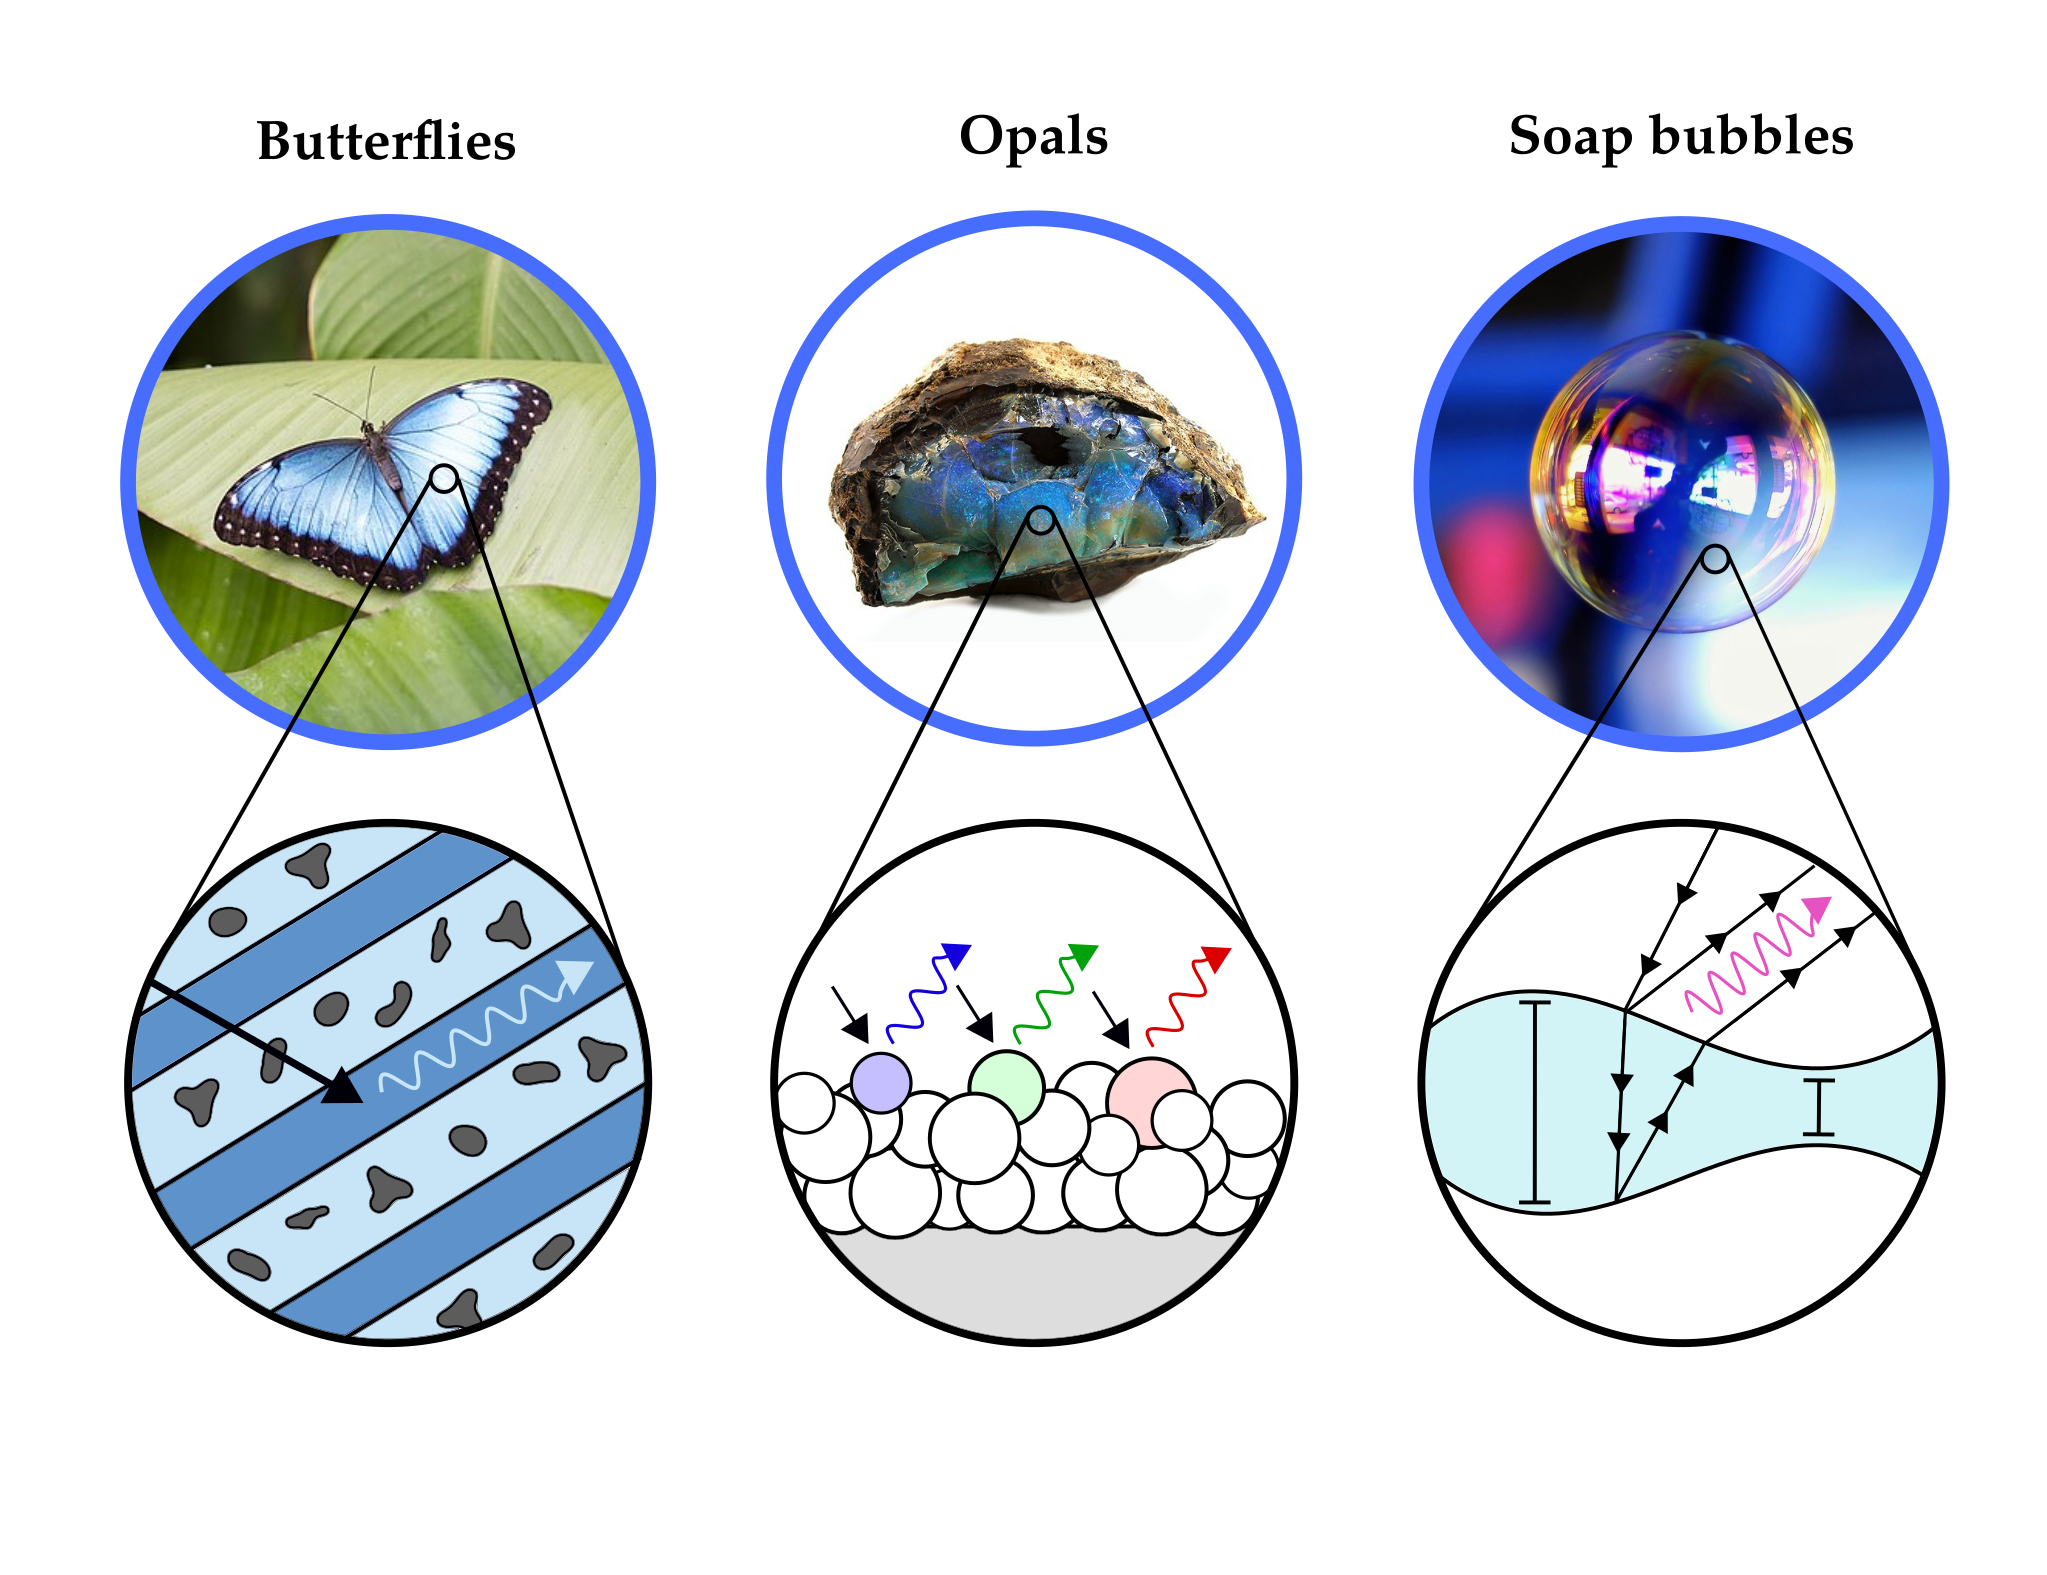
\includegraphics{figures/motivation_natural.png}}%%
    \caption{Examples of mascroscopic nano-optical systems that exhibit multi-physics effects. From left to right, nanostructures in wings of the butterfly, the colloidal crystal structure in the opal, and the thin-film effects in the varying thickness soap bubble.
    two colors in the soap bubble would work better visually! (Jens)}
    \label{fig:motivation_natural}
\end{figure}

% Wikimedia commons:
% 1. https://commons.wikimedia.org/wiki/File:Peleides_blue_morpho_(Morpho_peleides).jpg
% 2. https://commons.wikimedia.org/wiki/File:Opal-53714.jpg
% https://www.reddit.com/r/educationalgifs/comments/56sg9x/a_butterflys_wings_can_change_color_when_soaked/
%Sources:
%The GIF came from this video

%Ding, Y. Structural colors from Morpho peleides butterfly wing scales. J. Appl. Phys. 2009: 106, 074702

%Van Hooijdonk, E., et al. Detailed experimental analysis of the structural fluorescence in the butterfly Morpho sulkowskyi (Nymphalidae) J. Nanophoton. 2011: 5(1), 053525


The field of nano-optics ...

\section{Topology optimization in nano-optics}

As seen by the examples in Figure 1, nano-optical systems exhibit multi-physics effects,
where ingenously engineered geometry and material properties play a crucial role in the
optical response of the system. Inspired by these natural structures a goal of nano-optics
design is to optimize the geometry and material properties of the system to achieve a desired
optical response. Topology optimization offers a systematic approach to optimize the geometry
and material properties of a system to obtain a desired optical performance under a set of constraints.

Topology optimization is a systematic design method that can optimize designs based on a target FOM and a set of constraints. 
Say that it was introduced in the field of mechanics (CITE BENDSOE), but then it was extended to 
nano-optic and nanphotonic systems (CITE JENSEN, SIGMUND).

In Figure XX we we show an example of a topology optimziation problem in nano-optics. The 
main idea is two optimize the distribution of material in the design domain for two different materials, 
where the material distribution is optimized to maximize a FOM. ADD SOMETHING ABOUT THE SOURCE.


\begin{figure}[tb]
    \centering
    \makebox[\textwidth][c]{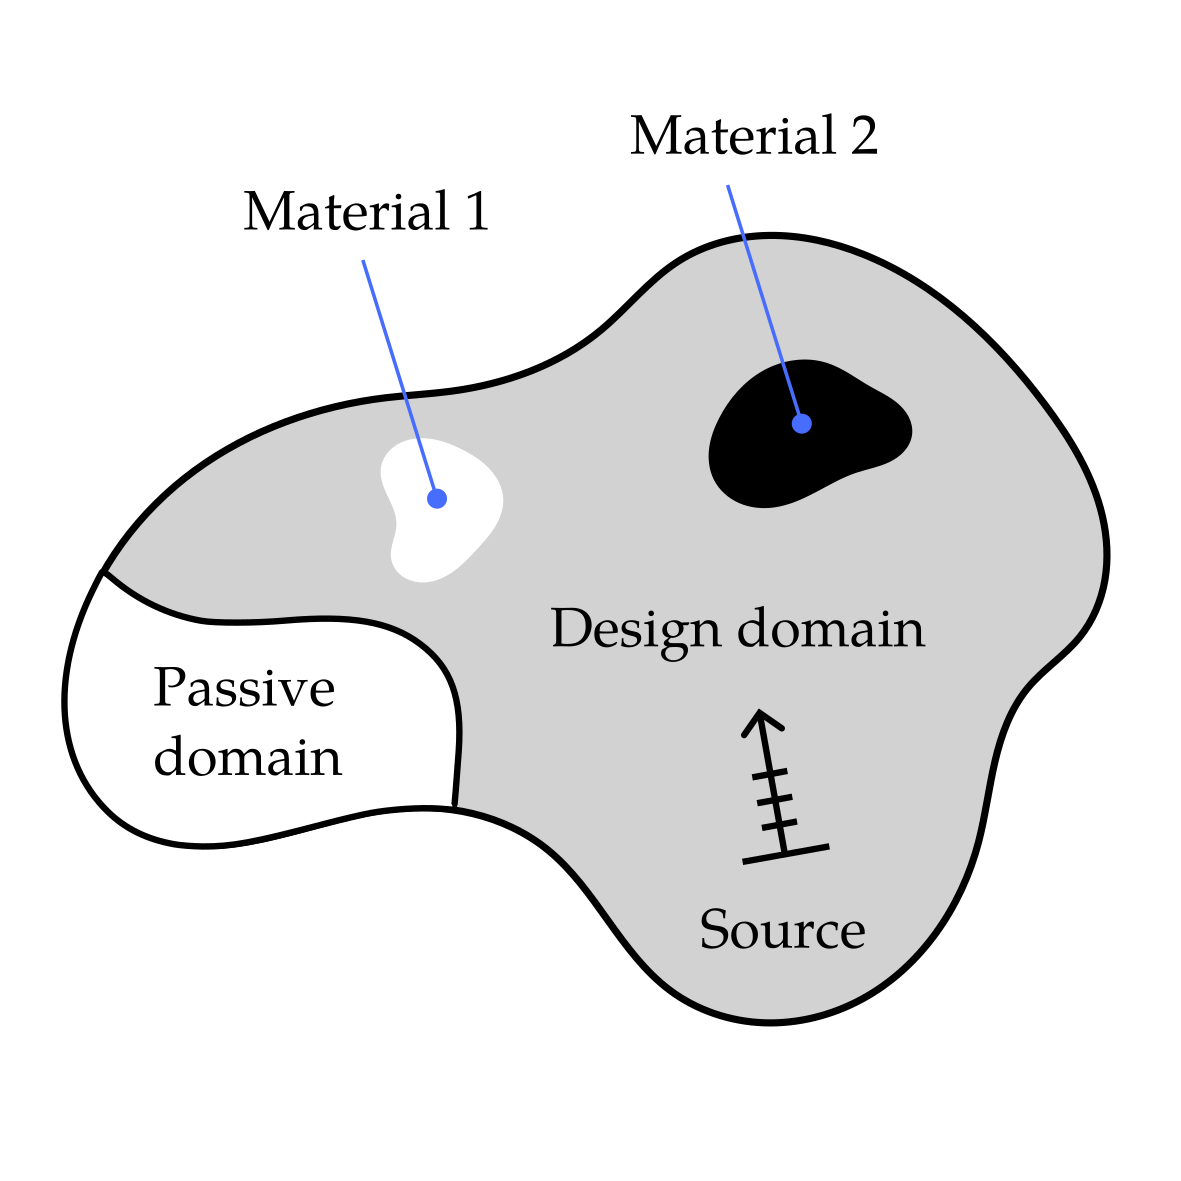
\includegraphics{figures/top_opt.png}}%%
    \caption{Topology optimization of a nano-optic system, excited by a source. The simulation domain is composed by a passive domain (blue) where the material is fixed, and a design domain (grey), where the material distribution is optimized for two different materials.}
    \label{fig:top_opt}
\end{figure}

\section{Structure of the Thesis}

This thesis covers multi-physics topology optimization problems in nano-optic systems. It provides an overview
of different type of multi-physics problems.

\textbf{Chapter 1} presents ...

\textbf{Chapter 2} presents ...

This thesis consists of a collection of papers, including unpublished work on
systems of coupled dipole emitter problems. The published content is included in the attached
papers.
\openright
\chapter{Theoretical framework}

Bla bla bla...

%\begin{figure}[tb]
%    \centering
%    \makebox[\textwidth][c]{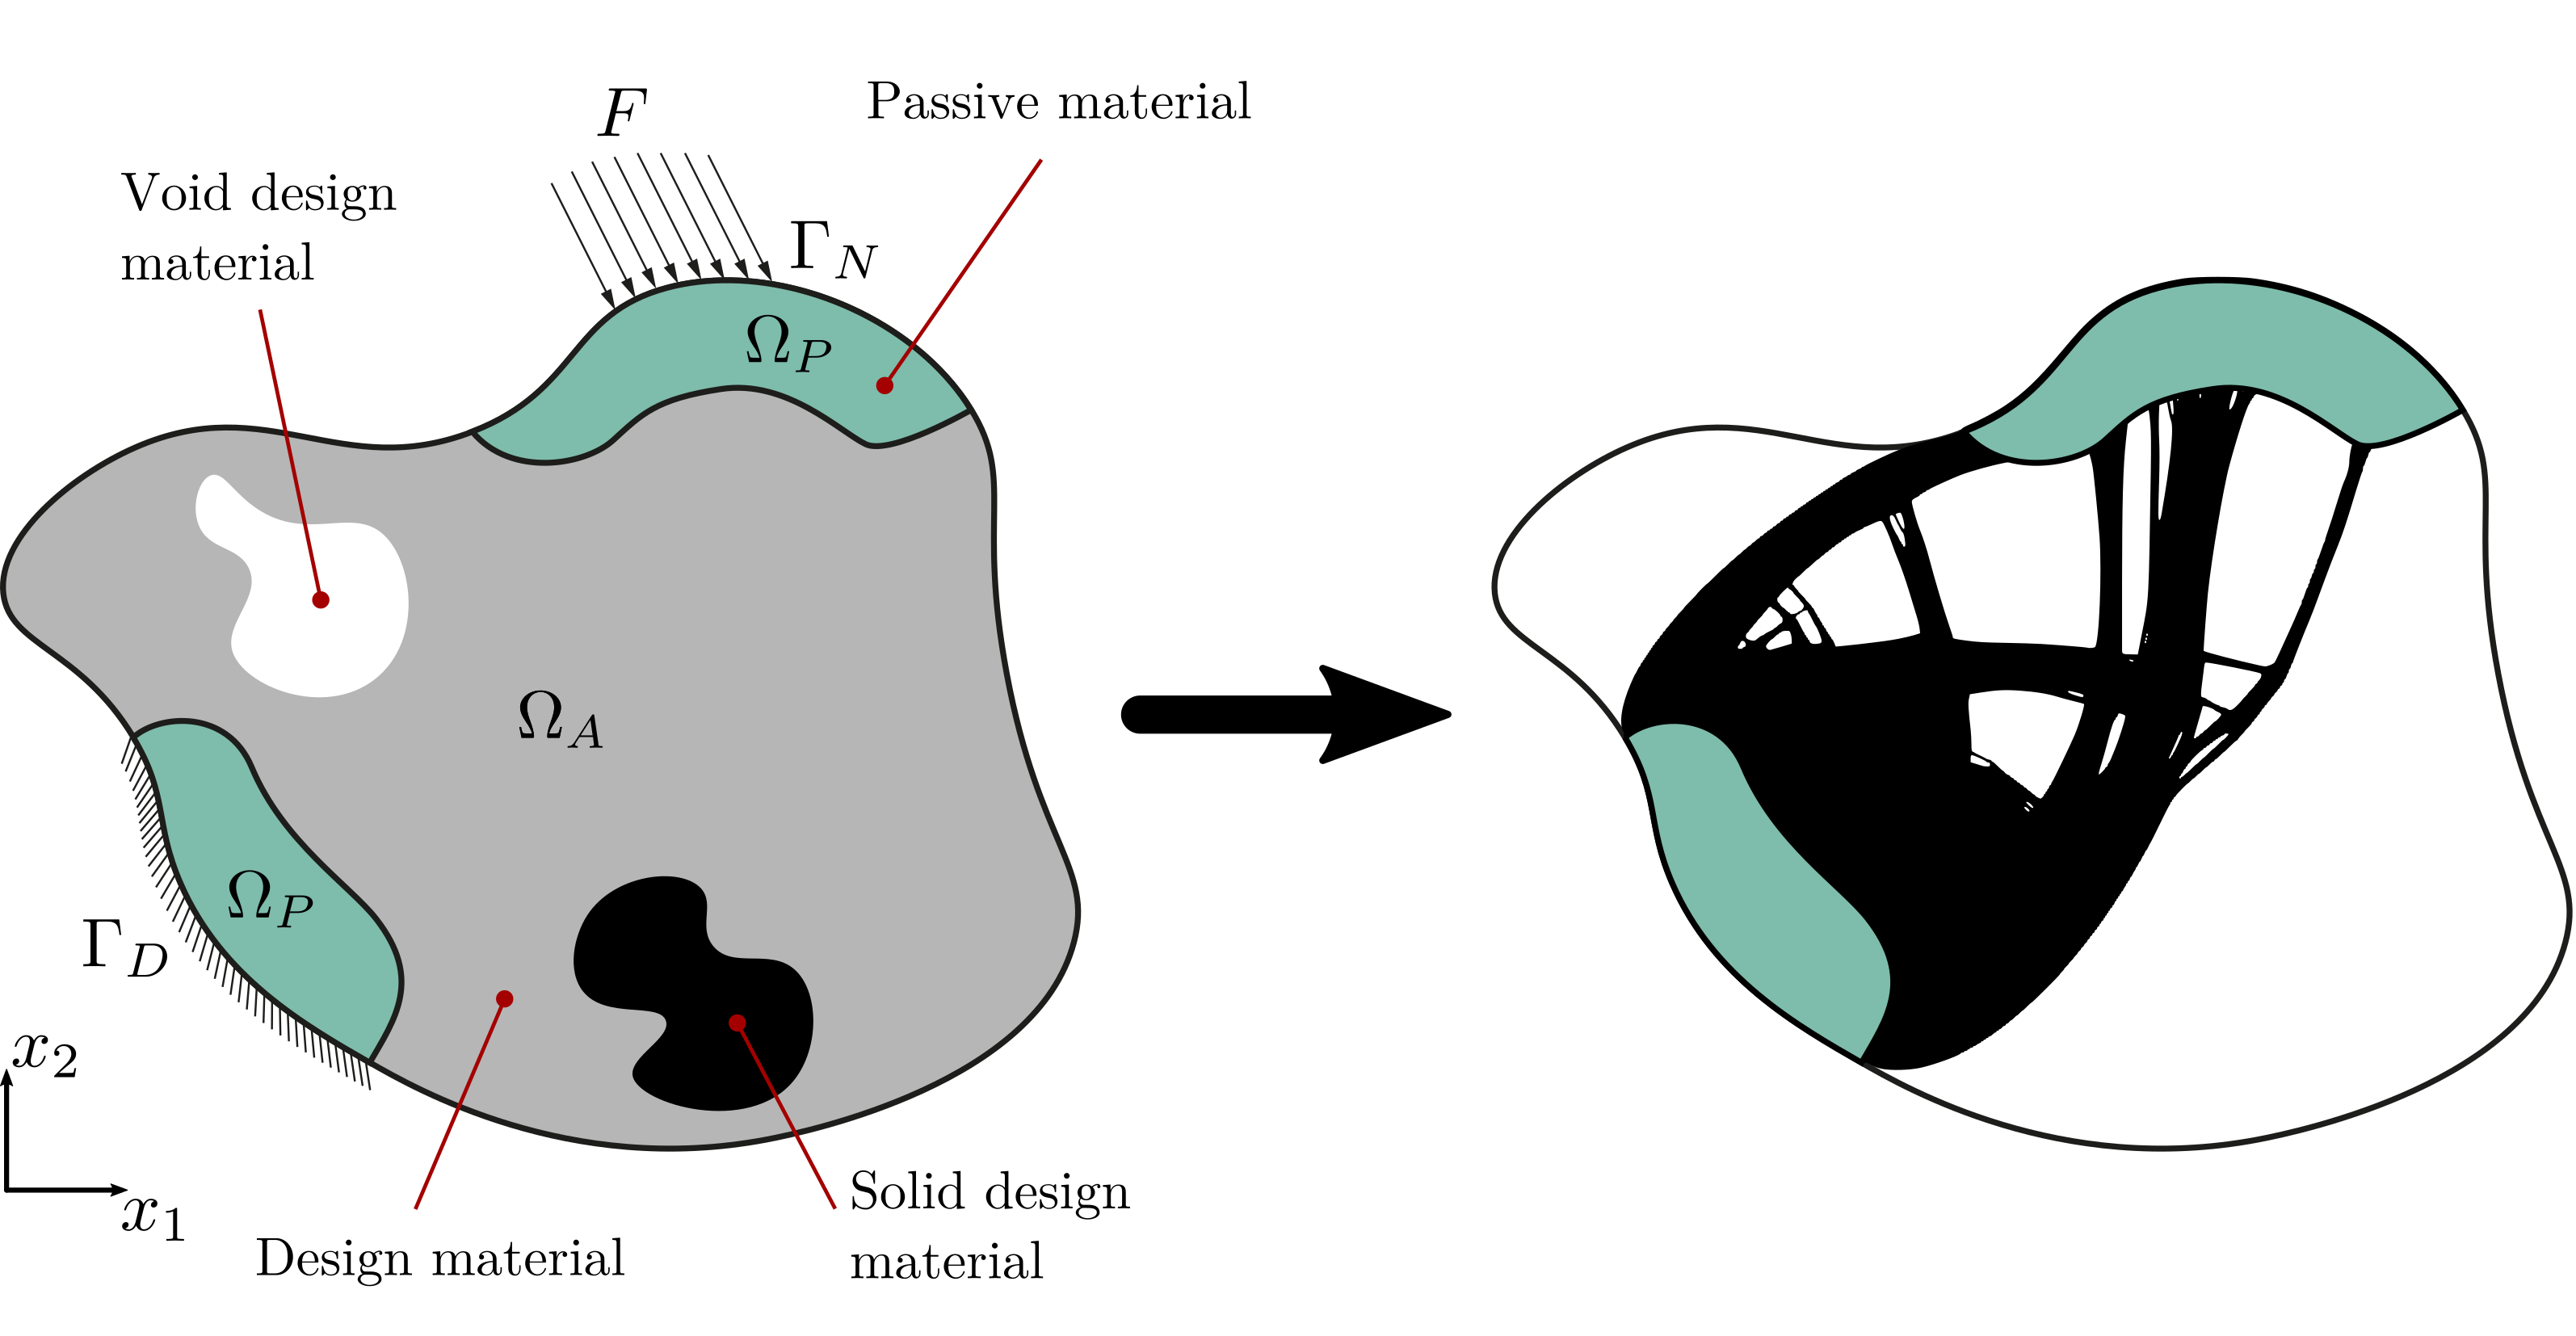
\includegraphics[width=1\imwidth]{figures/simpModel.png}}%
%    \caption{Bla bla bla...}
%    \label{fig:illustateTopOpt}
%\end{figure}


%\begin{equation}
%    (EIu'')'' = q
%\end{equation}


%\begin{figure}[tb]
%    \centering
%    \makebox[\textwidth][c]{\begin{tikzpicture}[remember picture]
    \begin{scope}[xshift=0mm]
        % angle (deg)
        \newcommand\ai{10}
        % line width
        \newcommand\wi{1pt}
        % cell size
        \newcommand\cellsize{3}
        % Rank-$N$ size
        \newcommand\di{0.75}

        % cell
        \draw[gray!10,   fill=gray!10, rotate around={\ai:(0,0)}] (0,0) rectangle (\cellsize,\cellsize) node (rect1) {};
        \draw[black!60, fill=black!60, rotate around={\ai:(0,0)}] (0,0) rectangle (\di,\cellsize);

        % orientation frame
        \draw[black, -stealth, line width=\wi, rotate around={\ai:({\di*cos(\ai) - \cellsize/2*sin(\ai)},{\di*sin(\ai) + \cellsize/2*cos(\ai)})}] ({\di*cos(\ai) - \cellsize/2*sin(\ai)},{\di*sin(\ai) + \cellsize/2*cos(\ai)}) -- ({\di*cos(\ai) - \cellsize/2*sin(\ai) + 0.75},{\di*sin(\ai) + \cellsize/2*cos(\ai)});
        \draw[black, -stealth, line width=\wi, rotate around={\ai:({\di*cos(\ai) - \cellsize/2*sin(\ai)},{\di*sin(\ai) + \cellsize/2*cos(\ai)})}] ({\di*cos(\ai) - \cellsize/2*sin(\ai)},{\di*sin(\ai) + \cellsize/2*cos(\ai)}) -- ({\di*cos(\ai) - \cellsize/2*sin(\ai)},{\di*sin(\ai) + \cellsize/2*cos(\ai) + 0.75});

        % local frame
        \draw[black, -stealth, dashed, line width=\wi] (0,0) -- ({\cellsize + 0.8},0);
        \draw[black, -stealth, dashed, line width=\wi] (0,0) -- (0,{\cellsize + 0.8});

        % ruler
        \draw[black, |-|, line width=\wi, rotate around={\ai:(0,0)}] (0,0) -- (\cellsize,0);
        \draw[black,  -|, line width=\wi, rotate around={\ai:(0,0)}] (0,0) -- (\di,0);

        % arc
        \draw[black, dotted, line width=\wi] (\cellsize,0) arc (0:\ai:\cellsize);

        % annotation
        \draw (\cellsize + 0.7, -0.3) node {$x_1 / \epsilon^3$};
        \draw (-0.5, \cellsize + 0.8) node {$x_2 / \epsilon^3$};
        \draw (\cellsize/2,-0.75) node {Rank-$1$};

        \draw[rotate around={{\ai/2}:(0,0)}] ({\cellsize+0.3},0) node {$\theta_1$};

        \draw[rotate around={{\ai}:(0,0)}] ({\di/2},0.4) node [rotate around={{\ai}:(0,0)}] {$\mu_1$};
        \draw[rotate around={{\ai}:(0,0)}] ({(\cellsize - \di)/2 + \di},0.4) node [rotate around={{\ai}:(0,0)}] {$1-\mu_1$};

        \draw[rotate around={{\ai}:(0,0)}] ({0+0.4},{\cellsize-0.4}) node [rotate around={{\ai}:(0,0)}] {$(+)$};
        \draw[rotate around={{\ai}:(0,0)}] ({\cellsize-0.4},{\cellsize-0.4}) node [rotate around={{\ai}:(0,0)}] {$(-)$};
        \coordinate (A) at (rect1.north);


        \draw[rotate around={\ai:({\di*cos(\ai) - \cellsize/2*sin(\ai)},{\di*sin(\ai) + \cellsize/2*cos(\ai)})}] ({\di*cos(\ai) - \cellsize/2*sin(\ai)+1} , {\di*sin(\ai) + \cellsize/2*cos(\ai) + 0.2}) node {$\mathbf{n}_1$};
        \draw[rotate around={\ai:({\di*cos(\ai) - \cellsize/2*sin(\ai)},{\di*sin(\ai) + \cellsize/2*cos(\ai)})}] ({\di*cos(\ai) - \cellsize/2*sin(\ai) + 0.3} , {\di*sin(\ai) + \cellsize/2*cos(\ai) + 1}) node {$\mathbf{m}_1$};



    \end{scope}
    \begin{scope}[xshift=45mm]
        % angle (deg)
        \newcommand\ai{15}
        % line width
        \newcommand\wi{1pt}
        % cell size
        \newcommand\cellsize{3}
        % Rank-$N$ size
        \newcommand\di{0.6}

        % cell
        \draw[gray!40,   fill=gray!40, rotate around={\ai:(0,0)}] (0,0) rectangle (\cellsize,\cellsize) node (rect2) {};
        \draw[black!60, fill=black!60, rotate around={\ai:(0,0)}] (0,0) rectangle (\di,\cellsize);

        % orientation frame
        \draw[black, -stealth, line width=\wi, rotate around={\ai:({\di*cos(\ai) - \cellsize/2*sin(\ai)},{\di*sin(\ai) + \cellsize/2*cos(\ai)})}] ({\di*cos(\ai) - \cellsize/2*sin(\ai)},{\di*sin(\ai) + \cellsize/2*cos(\ai)}) -- ({\di*cos(\ai) - \cellsize/2*sin(\ai) + 0.75},{\di*sin(\ai) + \cellsize/2*cos(\ai)});
        \draw[black, -stealth, line width=\wi, rotate around={\ai:({\di*cos(\ai) - \cellsize/2*sin(\ai)},{\di*sin(\ai) + \cellsize/2*cos(\ai)})}] ({\di*cos(\ai) - \cellsize/2*sin(\ai)},{\di*sin(\ai) + \cellsize/2*cos(\ai)}) -- ({\di*cos(\ai) - \cellsize/2*sin(\ai)},{\di*sin(\ai) + \cellsize/2*cos(\ai) + 0.75});

        % local frame
        \draw[black, -stealth, dashed, line width=\wi] (0,0) -- ({\cellsize + 0.8},0);
        \draw[black, -stealth, dashed, line width=\wi] (0,0) -- (0,{\cellsize + 0.8});

        % ruler
        \draw[black, |-|, line width=\wi, rotate around={\ai:(0,0)}] (0,0) -- (\cellsize,0);
        \draw[black,  -|, line width=\wi, rotate around={\ai:(0,0)}] (0,0) -- (\di,0);

        % arc
        \draw[black, dotted, line width=\wi] (\cellsize,0) arc (0:\ai:\cellsize);

        % annotation
        \draw (\cellsize + 0.7, -0.3) node {$x_1 / \epsilon^2$};
        \draw (-0.5, \cellsize + 0.8) node {$x_2 / \epsilon^2$};
        \draw (\cellsize/2,-0.75) node {Rank-$2$};

        \draw[rotate around={{\ai/2}:(0,0)}] ({\cellsize+0.3},0) node {$\theta_2 + \pi/4$};

        \draw[rotate around={{\ai}:(0,0)}] ({\di/2},0.4) node [rotate around={{\ai}:(0,0)}] {$\mu_2$};
        \draw[rotate around={{\ai}:(0,0)}] ({(\cellsize - \di)/2 + \di},0.4) node [rotate around={{\ai}:(0,0)}] {$1-\mu_2$};

        \draw[rotate around={{\ai}:(0,0)}] ({0+0.4},{\cellsize-0.4}) node [rotate around={{\ai}:(0,0)}] {$(+)$};
        \draw[rotate around={{\ai}:(0,0)}] ({\cellsize-0.9},{\cellsize-0.4}) node [rotate around={{\ai}:(0,0)}] (B) {$(\text{Rank-1})$};
        \coordinate (B2) at (rect2.north);


        \draw[rotate around={\ai:({\di*cos(\ai) - \cellsize/2*sin(\ai)},{\di*sin(\ai) + \cellsize/2*cos(\ai)})}] ({\di*cos(\ai) - \cellsize/2*sin(\ai)+1} , {\di*sin(\ai) + \cellsize/2*cos(\ai) + 0.2}) node {$\mathbf{n}_2$};
        \draw[rotate around={\ai:({\di*cos(\ai) - \cellsize/2*sin(\ai)},{\di*sin(\ai) + \cellsize/2*cos(\ai)})}] ({\di*cos(\ai) - \cellsize/2*sin(\ai) + 0.3} , {\di*sin(\ai) + \cellsize/2*cos(\ai) + 1}) node {$\mathbf{m}_2$};


    \end{scope}
    \begin{scope}[xshift=90mm]
        % angle (deg)
        \newcommand\ai{20}
        % line width
        \newcommand\wi{1pt}
        % cell size
        \newcommand\cellsize{3}
        % Rank-$N$ size
        \newcommand\di{1.0}

        % cell
        \draw[gray!60,   fill=gray!60, rotate around={\ai:(0,0)}] (0,0) rectangle (\cellsize,\cellsize);
        \draw[black!60, fill=black!60, rotate around={\ai:(0,0)}] (0,0) rectangle (\di,\cellsize);

        % orientation frame
        \draw[black, -stealth, line width=\wi, rotate around={\ai:({\di*cos(\ai) - \cellsize/2*sin(\ai)},{\di*sin(\ai) + \cellsize/2*cos(\ai)})}] ({\di*cos(\ai) - \cellsize/2*sin(\ai)},{\di*sin(\ai) + \cellsize/2*cos(\ai)}) -- ({\di*cos(\ai) - \cellsize/2*sin(\ai) + 0.75},{\di*sin(\ai) + \cellsize/2*cos(\ai)});
        \draw[black, -stealth, line width=\wi, rotate around={\ai:({\di*cos(\ai) - \cellsize/2*sin(\ai)},{\di*sin(\ai) + \cellsize/2*cos(\ai)})}] ({\di*cos(\ai) - \cellsize/2*sin(\ai)},{\di*sin(\ai) + \cellsize/2*cos(\ai)}) -- ({\di*cos(\ai) - \cellsize/2*sin(\ai)},{\di*sin(\ai) + \cellsize/2*cos(\ai) + 0.75});

        % local frame
        \draw[black, -stealth, dashed, line width=\wi] (0,0) -- ({\cellsize + 0.8},0);
        \draw[black, -stealth, dashed, line width=\wi] (0,0) -- (0,{\cellsize + 0.8});

        % ruler
        \draw[black, |-|, line width=\wi, rotate around={\ai:(0,0)}] (0,0) -- (\cellsize,0);
        \draw[black,  -|, line width=\wi, rotate around={\ai:(0,0)}] (0,0) -- (\di,0);

        % arc
        \draw[black, dotted, line width=\wi] (\cellsize,0) arc (0:\ai:\cellsize);

        % annotation
        \draw (\cellsize + 0.7, -0.3) node {$x_1 / \epsilon$};
        \draw (-0.5, \cellsize + 0.8) node {$x_2 / \epsilon$};
        \draw (\cellsize/2,-0.75) node {Rank-$3$};

        \draw[rotate around={{\ai/2}:(0,0)}] ({\cellsize+0.3},0) node {$\theta_3 - \pi/2$};

        \draw[rotate around={{\ai}:(0,0)}] ({\di/2},0.4) node [rotate around={{\ai}:(0,0)}] {$\mu_3$};
        \draw[rotate around={{\ai}:(0,0)}] ({(\cellsize - \di)/2 + \di},0.4) node [rotate around={{\ai}:(0,0)}] {$1-\mu_3$};

        \draw[rotate around={{\ai}:(0,0)}] ({0+0.4},{\cellsize-0.4}) node [rotate around={{\ai}:(0,0)}] {$(+)$};
        \draw[rotate around={{\ai}:(0,0)}] ({\cellsize-0.9},{\cellsize-0.4}) node [rotate around={{\ai}:(0,0)}] (C) {$(\text{Rank-2})$};


        \draw[rotate around={\ai:({\di*cos(\ai) - \cellsize/2*sin(\ai)},{\di*sin(\ai) + \cellsize/2*cos(\ai)})}] ({\di*cos(\ai) - \cellsize/2*sin(\ai)+1} , {\di*sin(\ai) + \cellsize/2*cos(\ai) + 0.2}) node {$\mathbf{n}_3$};
        \draw[rotate around={\ai:({\di*cos(\ai) - \cellsize/2*sin(\ai)},{\di*sin(\ai) + \cellsize/2*cos(\ai)})}] ({\di*cos(\ai) - \cellsize/2*sin(\ai) + 0.3} , {\di*sin(\ai) + \cellsize/2*cos(\ai) + 1}) node {$\mathbf{m}_3$};

    \end{scope}
    \path[-latex,black,thick] (A) edge [bend left=50] (B);
    \path[-latex,black,thick] (B2) edge [bend left=50] (C);
\end{tikzpicture}}%
%    \caption{Bla bla bla...}
%    \label{fig:Rank}
%\end{figure}

\section{Modeling optical systems -- an electromagnetic wave problem}

\subsection*{The macroscopic Maxwell's equations}

Macroscopic electromagnetic systems can be described by Maxwell's equations. The time-domain Maxwell's equations in a linear, isotropic, and homogeneous medium can be written as
\begin{align}
    \nabla \times \mathbf{E} (\mathbf{r},t) &= - \frac{\partial \mathbf{B}(\mathbf{r},t)}{\partial t}, \quad \quad &\text{(Faraday's law)} \label{eq:curlE_time}\\
    \nabla \times \mathbf{H} (\mathbf{r},t) &= \varepsilon \frac{\partial \mathbf{E}(\mathbf{r},t)}{\partial t} + \mathbf{j}(\mathbf{r},t), \quad \quad &\text{(Ampère's law)} \label{eq:curlH_time}\\
    \nabla \cdot \mathbf{D} (\mathbf{r},t) &= \rho(\mathbf{r},t), \quad \quad &\text{(Gauss's law for electricity)} \label{eq:divD_time}\\
    \nabla \cdot \mathbf{B} (\mathbf{r},t) &= 0, \quad \quad &\text{(Gauss's law for magnetism)} \label{eq:divB_time}
\end{align}
where $\mathbf{E}$ and $\mathbf{H}$ are the electric and magnetic fields, respectively, $\mathbf{D} = \varepsilon \mathbf{E}$ is the electric displacement field, $\mathbf{B} = \mu \mathbf{H}$ is the magnetic induction field, $\varepsilon$ is the permittivity, and $\mu$ is the permeability.

In the presence of polarization $\mathbf{P}$ and magnetization $\mathbf{M}$, the fields $\mathbf{D}$ and $\mathbf{B}$ are related to $\mathbf{E}$ and $\mathbf{H}$ by $\mathbf{D}(\mathbf{r}, t) = \varepsilon_0 \mathbf{E}(\mathbf{r}, t) + \mathbf{P}(\mathbf{r}, t)$ and $\mathbf{H}(\mathbf{r}, t) = \mu_0^{-1} \mathbf{B}(\mathbf{r}, t) - \mathbf{M}(\mathbf{r}, t)$

where $\varepsilon_0$ is the permittivity of free space and $\mu_0$ is the permeability of free space.


\subsection*{Electromagnetics in the frequency domain}

The time-dependence in Maxwell's equations can be separated by assuming a harmonic time-dependence of the fields:

\begin{equation}
    \mathbf{E}(\mathbf{r}, t) = \Re \{ \mathbf{E}(\mathbf{r}) e^{-i\omega t} \} = \frac{1}{2}\left[ \mathbf{E}(\mathbf{r}) e^{i\omega t} + \mathbf{E}^*(\mathbf{r}) e^{-i\omega t}\right], \label{eq:E_harmonic}\\
\end{equation}

Then, the time-domain Maxwell's equations can be written as

\begin{align}
    \nabla \times \mathbf{E} &= -i\omega \mu \mathbf{H}, \quad \quad &\text{(Faraday's law)} \label{eq:curlE_freq}\\
    \nabla \times \mathbf{H} &= i\omega \varepsilon \mathbf{E}, \quad \quad &\text{(Ampère's law)} \label{eq:curlH_freq}\\
    \nabla \cdot \mathbf{D} &= 0, \quad \quad &\text{(Gauss's law for electricity)} \label{eq:divD_freq}\\
    \nabla \cdot \mathbf{B} &= 0, \quad \quad &\text{(Gauss's law for magnetism)} \label{eq:divB_freq}
\end{align}

WRITE WAVE EQUATION

\subsection*{Piecewise homogeneous media and boundary conditions}

\subsection*{Modeling single emitters: the Green's function formalism}

\subsection*{Some useful properties of Maxwell's equations}

Linearity, superposition, conservation laws (charge, energy, momentum), time-reversal symmetry/recirpocity
self-adjointness, duality symmetry ...

\subsection*{Point-like emitters: the Green's function formalism}

\section{The finite element method in electromagnetics}

(CHECK IANS THESIS)

The weak form of the wave equation can be written as (CHECK CHATGPT):
\begin{equation}
    \int_{\Omega} \nabla \times \mathbf{E} \cdot \nabla \times \mathbf{v} - k^2 \int_{\Omega} \mathbf{E} \cdot \mathbf{v} = \int_{\Omega} \mathbf{J} \cdot \mathbf{v} \quad \forall \mathbf{v} \in V,
\end{equation}
The weak form can be discretized by using the finite-element method. An example is shown in Figure YY, 
where we have discretized the two-dimensional domain in Figure XX into a set of triangular edge elements. 
The edge elements, or Nedelec elements (CITE), of first kind are a natural choice for the electromagnetic 
wave equation, as they are divergence-free and enforce the continuity of the tangential electric field 
across the element boundaries, which is a natural boundary condition for Maxwell's equations 
\footnote{For 2D models where the field discontinuity at the material interfaces 
is in the out-of-plane direction (e.g., Publication 3), one can use Lagrange element without 
exciting spurious modes.}. In Figure YY
we show the structure of a Nedelec element alongside a quiver plot of the shape function one of the edges.
Using the shape functions we can calculate the contribution of the different elements to the weak form of the
wave equation, which can be assembled into a system of equations in the strong form:
\begin{equation}
    \mathbf{K} \mathbf{E} = \mathbf{F},
\end{equation}
where $\mathbf{K}$ is the stiffness matrix, $\mathbf{E}$ is the electric field, and $\mathbf{F}$ is the source
 term. In the case of eigenvalue problems the source term is zero ($\mathbf{F}=0$), and the system of equations 
that needs to be solved is given by:
\begin{equation}
    \left(\mathbf{K} - \lambda \mathbf{I} \right) \mathbf{E} =  \mathbf{0},
\end{equation}

Note that the stiffness matrix is symmetric indefinite, restricting the use of iterative solvers (e.g., Cholesky factorization, Krylov method) to solve the system of equations. Instead LU factorization is a common choice for direct solvers.
\begin{figure}[tb]
    \centering
    \makebox[\textwidth][c]{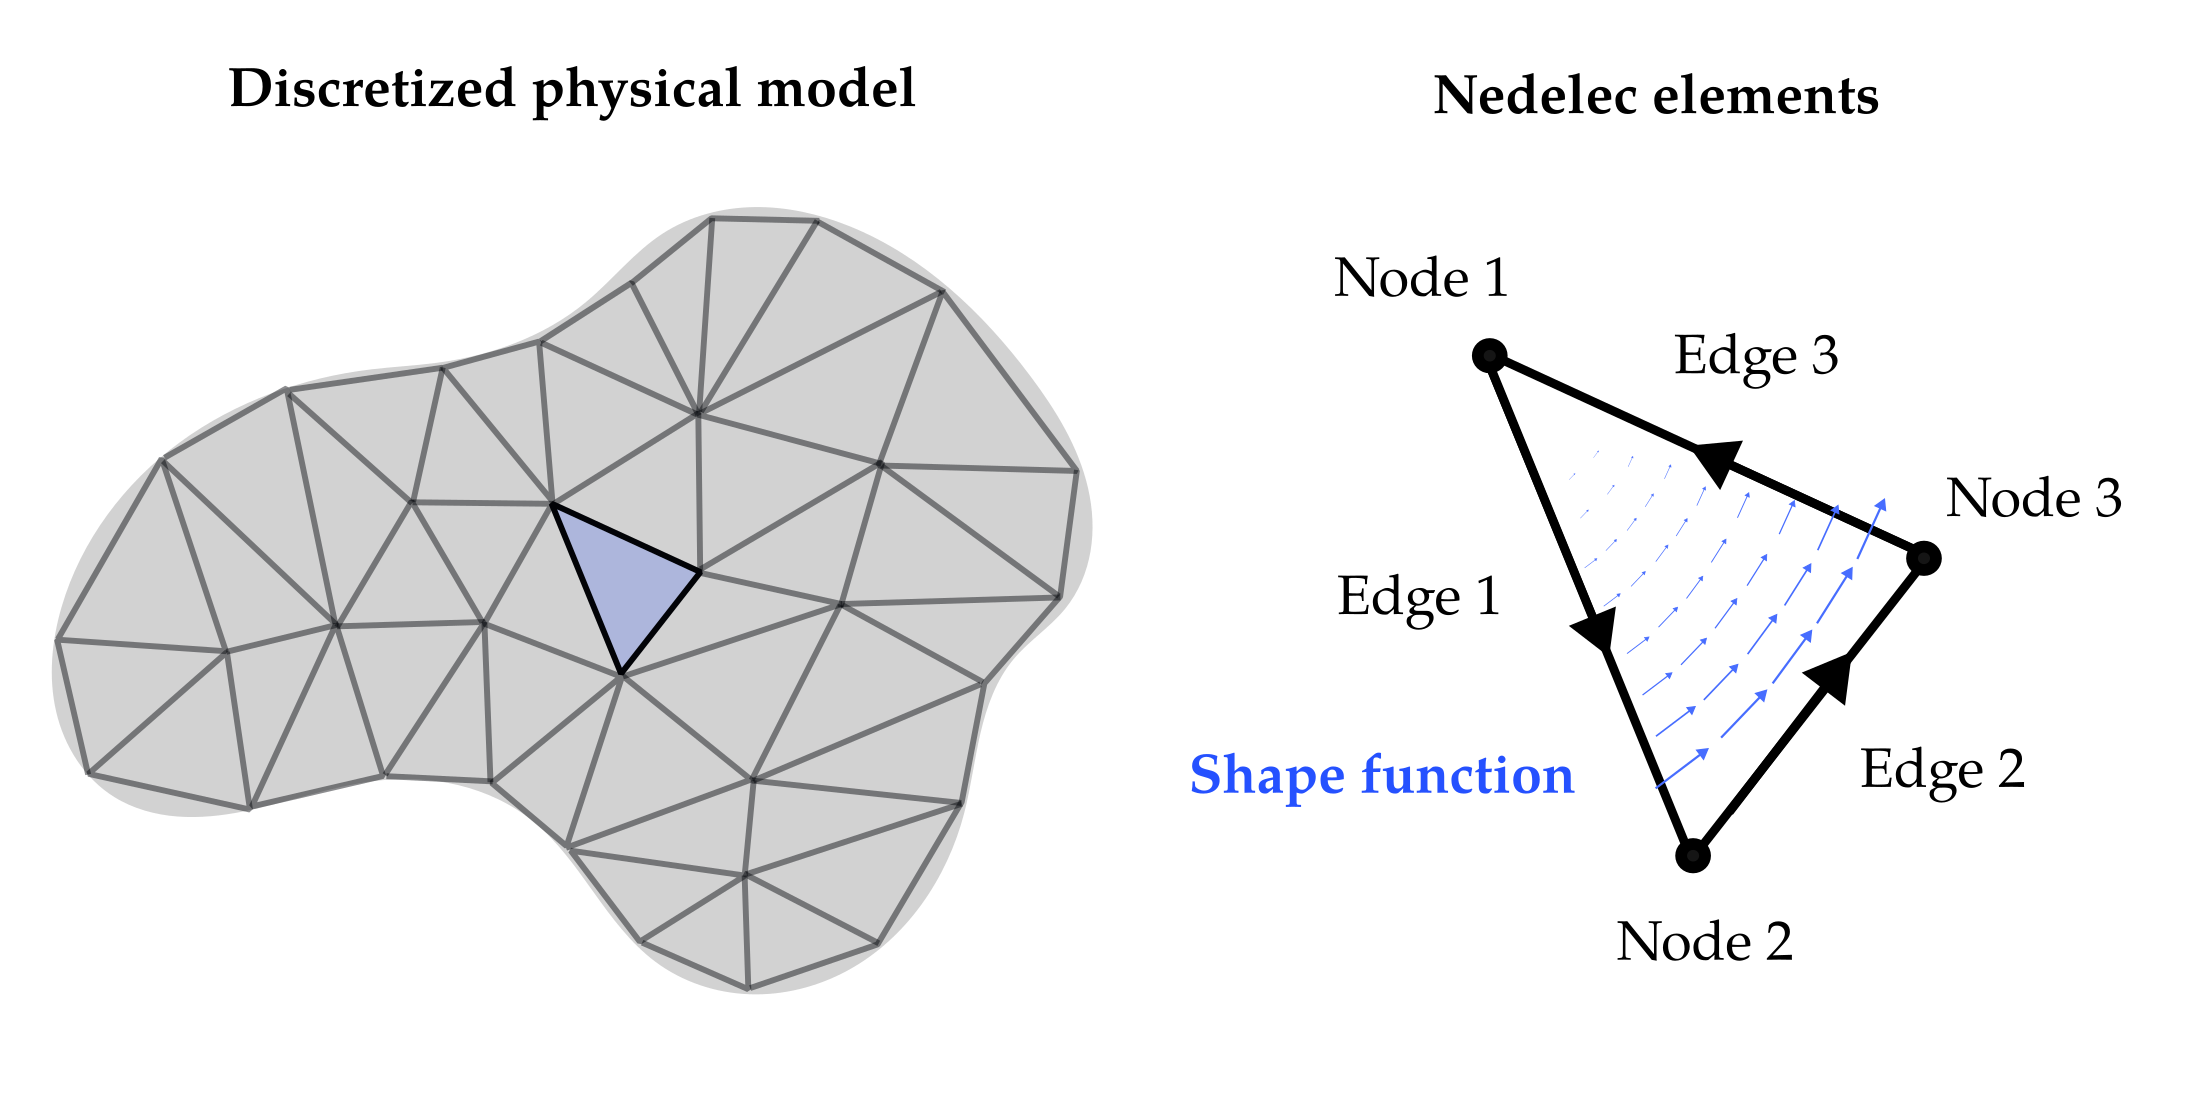
\includegraphics{figures/FEM.png}}%%
    \caption{Geometrical discretization of the physical domain into the finite element mesh, which is composed of Nedelec vector-elements. The element colored in light blue is a triangular element with three nodes and three edges, where we have sketched a quiver plot for the shape function $\mathbf{N}_2$ for Edge 2.}
    \label{fig:fem}
\end{figure}

Eigenvalue vs RHS problems


Lagrange elements vs Edge elements. Comment spurious modes.

\section{Beyond single-physics -- coupled optical systems}

Differentiate between weak and strong coupling.

\section{Topology optimization of multiphysics systems}

\subsection{Adjoint sensitivity analysis}

\section{A practical note on computational implementation}

Using first order edge, or nodal, elements a rule of thumb is to include at least 10 elements per wavelength.

Discuss direct vs iterative solvers, discuss condition number of the system.
Sparsity, symmetry, definitiness
Discuss the practical implementation, with COMSOL and other means (Fenics, gridap, etc).
Check Niels, Ian's thesis, and other references.
Bla bla bla...
\openright
\chapter{Thermo-optical topology optimization problems}\label{chap:to}
%CHECK COPYRIGHT FOR FIGURES AND REPRINTS
%In this chapter we will focus on the effects of multiphysics couplings in nanophotonic devices, reviewing state-of-the-art research, 
%highlighting open topology optimization problems, and presenting our contributions to the field.
%We will focus on three main classes of multiphysics couplings: thermo-optical, opto-mechanical, and electro-optical systems.
%\begin{figure}[tb]
%    \centering
%    \makebox[\textwidth][c]{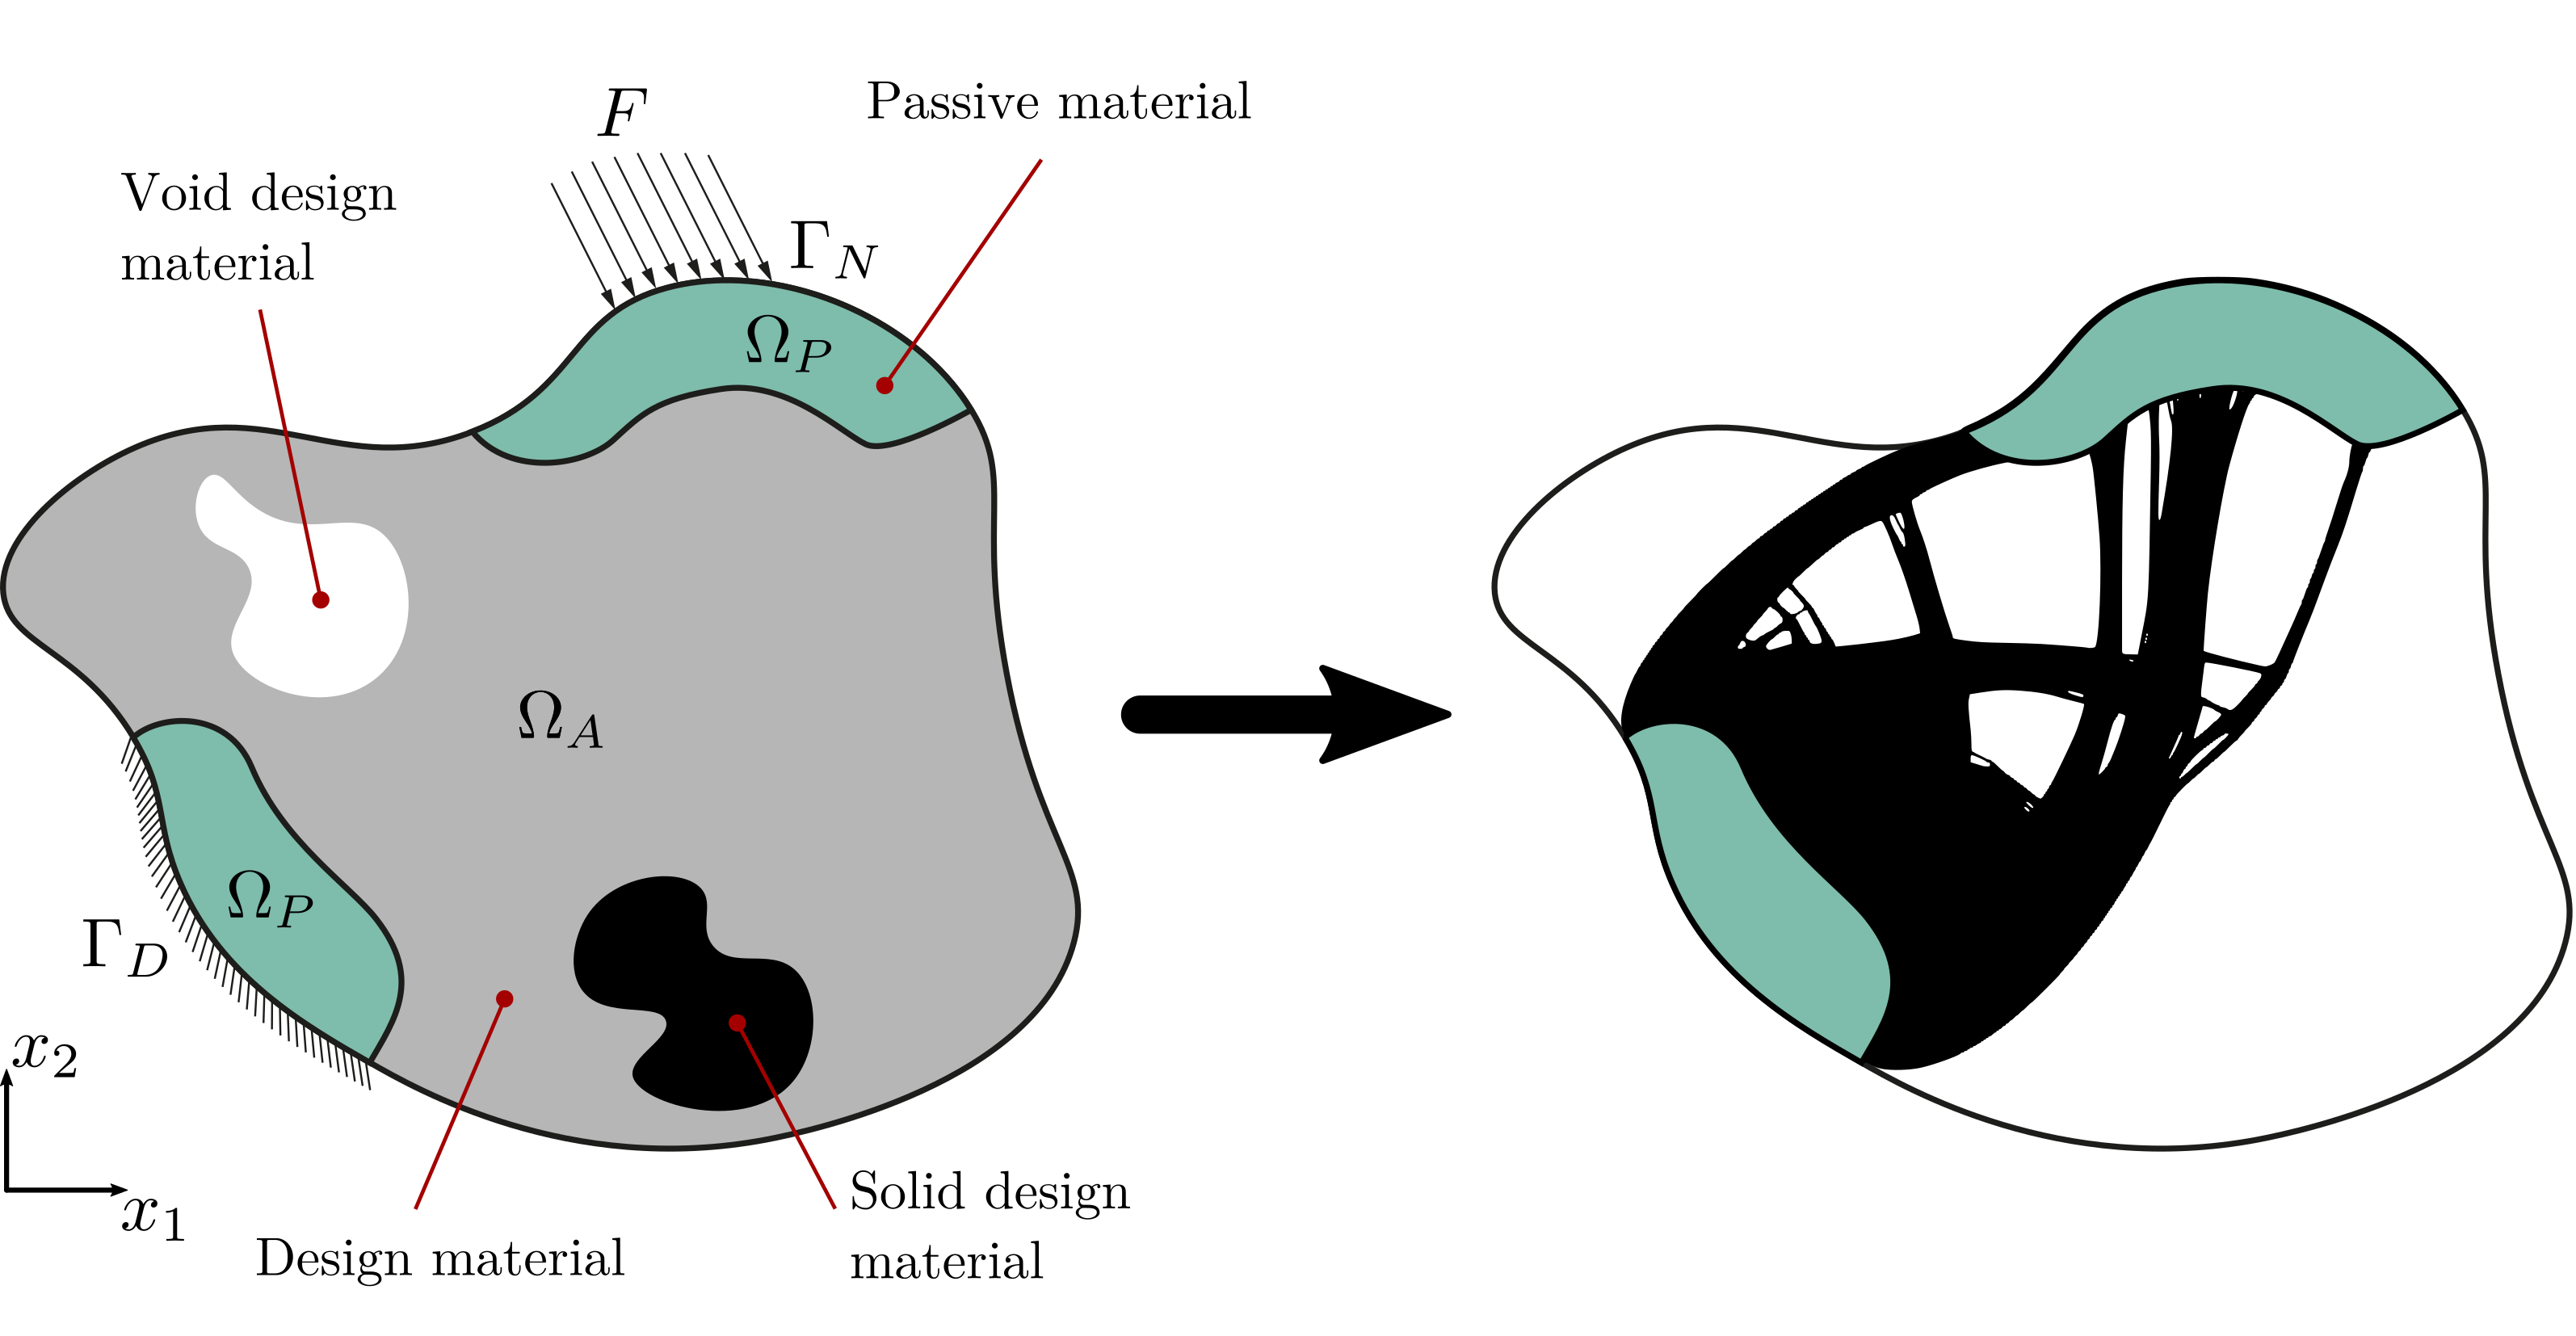
\includegraphics[width=1\imwidth]{figures/simpModel.png}}%
%    \caption{Bla bla bla...}
%    \label{fig:illustateTopOpt}
%\end{figure
%\begin{equation}
%    (EIu'')'' = q
%\end{equation}
%\beginfigure}[tb]
%    \centering
%    \makebox[\textwidth][c]{\begin{tikzpicture}[remember picture]
    \begin{scope}[xshift=0mm]
        % angle (deg)
        \newcommand\ai{10}
        % line width
        \newcommand\wi{1pt}
        % cell size
        \newcommand\cellsize{3}
        % Rank-$N$ size
        \newcommand\di{0.75}

        % cell
        \draw[gray!10,   fill=gray!10, rotate around={\ai:(0,0)}] (0,0) rectangle (\cellsize,\cellsize) node (rect1) {};
        \draw[black!60, fill=black!60, rotate around={\ai:(0,0)}] (0,0) rectangle (\di,\cellsize);

        % orientation frame
        \draw[black, -stealth, line width=\wi, rotate around={\ai:({\di*cos(\ai) - \cellsize/2*sin(\ai)},{\di*sin(\ai) + \cellsize/2*cos(\ai)})}] ({\di*cos(\ai) - \cellsize/2*sin(\ai)},{\di*sin(\ai) + \cellsize/2*cos(\ai)}) -- ({\di*cos(\ai) - \cellsize/2*sin(\ai) + 0.75},{\di*sin(\ai) + \cellsize/2*cos(\ai)});
        \draw[black, -stealth, line width=\wi, rotate around={\ai:({\di*cos(\ai) - \cellsize/2*sin(\ai)},{\di*sin(\ai) + \cellsize/2*cos(\ai)})}] ({\di*cos(\ai) - \cellsize/2*sin(\ai)},{\di*sin(\ai) + \cellsize/2*cos(\ai)}) -- ({\di*cos(\ai) - \cellsize/2*sin(\ai)},{\di*sin(\ai) + \cellsize/2*cos(\ai) + 0.75});

        % local frame
        \draw[black, -stealth, dashed, line width=\wi] (0,0) -- ({\cellsize + 0.8},0);
        \draw[black, -stealth, dashed, line width=\wi] (0,0) -- (0,{\cellsize + 0.8});

        % ruler
        \draw[black, |-|, line width=\wi, rotate around={\ai:(0,0)}] (0,0) -- (\cellsize,0);
        \draw[black,  -|, line width=\wi, rotate around={\ai:(0,0)}] (0,0) -- (\di,0);

        % arc
        \draw[black, dotted, line width=\wi] (\cellsize,0) arc (0:\ai:\cellsize);

        % annotation
        \draw (\cellsize + 0.7, -0.3) node {$x_1 / \epsilon^3$};
        \draw (-0.5, \cellsize + 0.8) node {$x_2 / \epsilon^3$};
        \draw (\cellsize/2,-0.75) node {Rank-$1$};

        \draw[rotate around={{\ai/2}:(0,0)}] ({\cellsize+0.3},0) node {$\theta_1$};

        \draw[rotate around={{\ai}:(0,0)}] ({\di/2},0.4) node [rotate around={{\ai}:(0,0)}] {$\mu_1$};
        \draw[rotate around={{\ai}:(0,0)}] ({(\cellsize - \di)/2 + \di},0.4) node [rotate around={{\ai}:(0,0)}] {$1-\mu_1$};

        \draw[rotate around={{\ai}:(0,0)}] ({0+0.4},{\cellsize-0.4}) node [rotate around={{\ai}:(0,0)}] {$(+)$};
        \draw[rotate around={{\ai}:(0,0)}] ({\cellsize-0.4},{\cellsize-0.4}) node [rotate around={{\ai}:(0,0)}] {$(-)$};
        \coordinate (A) at (rect1.north);


        \draw[rotate around={\ai:({\di*cos(\ai) - \cellsize/2*sin(\ai)},{\di*sin(\ai) + \cellsize/2*cos(\ai)})}] ({\di*cos(\ai) - \cellsize/2*sin(\ai)+1} , {\di*sin(\ai) + \cellsize/2*cos(\ai) + 0.2}) node {$\mathbf{n}_1$};
        \draw[rotate around={\ai:({\di*cos(\ai) - \cellsize/2*sin(\ai)},{\di*sin(\ai) + \cellsize/2*cos(\ai)})}] ({\di*cos(\ai) - \cellsize/2*sin(\ai) + 0.3} , {\di*sin(\ai) + \cellsize/2*cos(\ai) + 1}) node {$\mathbf{m}_1$};



    \end{scope}
    \begin{scope}[xshift=45mm]
        % angle (deg)
        \newcommand\ai{15}
        % line width
        \newcommand\wi{1pt}
        % cell size
        \newcommand\cellsize{3}
        % Rank-$N$ size
        \newcommand\di{0.6}

        % cell
        \draw[gray!40,   fill=gray!40, rotate around={\ai:(0,0)}] (0,0) rectangle (\cellsize,\cellsize) node (rect2) {};
        \draw[black!60, fill=black!60, rotate around={\ai:(0,0)}] (0,0) rectangle (\di,\cellsize);

        % orientation frame
        \draw[black, -stealth, line width=\wi, rotate around={\ai:({\di*cos(\ai) - \cellsize/2*sin(\ai)},{\di*sin(\ai) + \cellsize/2*cos(\ai)})}] ({\di*cos(\ai) - \cellsize/2*sin(\ai)},{\di*sin(\ai) + \cellsize/2*cos(\ai)}) -- ({\di*cos(\ai) - \cellsize/2*sin(\ai) + 0.75},{\di*sin(\ai) + \cellsize/2*cos(\ai)});
        \draw[black, -stealth, line width=\wi, rotate around={\ai:({\di*cos(\ai) - \cellsize/2*sin(\ai)},{\di*sin(\ai) + \cellsize/2*cos(\ai)})}] ({\di*cos(\ai) - \cellsize/2*sin(\ai)},{\di*sin(\ai) + \cellsize/2*cos(\ai)}) -- ({\di*cos(\ai) - \cellsize/2*sin(\ai)},{\di*sin(\ai) + \cellsize/2*cos(\ai) + 0.75});

        % local frame
        \draw[black, -stealth, dashed, line width=\wi] (0,0) -- ({\cellsize + 0.8},0);
        \draw[black, -stealth, dashed, line width=\wi] (0,0) -- (0,{\cellsize + 0.8});

        % ruler
        \draw[black, |-|, line width=\wi, rotate around={\ai:(0,0)}] (0,0) -- (\cellsize,0);
        \draw[black,  -|, line width=\wi, rotate around={\ai:(0,0)}] (0,0) -- (\di,0);

        % arc
        \draw[black, dotted, line width=\wi] (\cellsize,0) arc (0:\ai:\cellsize);

        % annotation
        \draw (\cellsize + 0.7, -0.3) node {$x_1 / \epsilon^2$};
        \draw (-0.5, \cellsize + 0.8) node {$x_2 / \epsilon^2$};
        \draw (\cellsize/2,-0.75) node {Rank-$2$};

        \draw[rotate around={{\ai/2}:(0,0)}] ({\cellsize+0.3},0) node {$\theta_2 + \pi/4$};

        \draw[rotate around={{\ai}:(0,0)}] ({\di/2},0.4) node [rotate around={{\ai}:(0,0)}] {$\mu_2$};
        \draw[rotate around={{\ai}:(0,0)}] ({(\cellsize - \di)/2 + \di},0.4) node [rotate around={{\ai}:(0,0)}] {$1-\mu_2$};

        \draw[rotate around={{\ai}:(0,0)}] ({0+0.4},{\cellsize-0.4}) node [rotate around={{\ai}:(0,0)}] {$(+)$};
        \draw[rotate around={{\ai}:(0,0)}] ({\cellsize-0.9},{\cellsize-0.4}) node [rotate around={{\ai}:(0,0)}] (B) {$(\text{Rank-1})$};
        \coordinate (B2) at (rect2.north);


        \draw[rotate around={\ai:({\di*cos(\ai) - \cellsize/2*sin(\ai)},{\di*sin(\ai) + \cellsize/2*cos(\ai)})}] ({\di*cos(\ai) - \cellsize/2*sin(\ai)+1} , {\di*sin(\ai) + \cellsize/2*cos(\ai) + 0.2}) node {$\mathbf{n}_2$};
        \draw[rotate around={\ai:({\di*cos(\ai) - \cellsize/2*sin(\ai)},{\di*sin(\ai) + \cellsize/2*cos(\ai)})}] ({\di*cos(\ai) - \cellsize/2*sin(\ai) + 0.3} , {\di*sin(\ai) + \cellsize/2*cos(\ai) + 1}) node {$\mathbf{m}_2$};


    \end{scope}
    \begin{scope}[xshift=90mm]
        % angle (deg)
        \newcommand\ai{20}
        % line width
        \newcommand\wi{1pt}
        % cell size
        \newcommand\cellsize{3}
        % Rank-$N$ size
        \newcommand\di{1.0}

        % cell
        \draw[gray!60,   fill=gray!60, rotate around={\ai:(0,0)}] (0,0) rectangle (\cellsize,\cellsize);
        \draw[black!60, fill=black!60, rotate around={\ai:(0,0)}] (0,0) rectangle (\di,\cellsize);

        % orientation frame
        \draw[black, -stealth, line width=\wi, rotate around={\ai:({\di*cos(\ai) - \cellsize/2*sin(\ai)},{\di*sin(\ai) + \cellsize/2*cos(\ai)})}] ({\di*cos(\ai) - \cellsize/2*sin(\ai)},{\di*sin(\ai) + \cellsize/2*cos(\ai)}) -- ({\di*cos(\ai) - \cellsize/2*sin(\ai) + 0.75},{\di*sin(\ai) + \cellsize/2*cos(\ai)});
        \draw[black, -stealth, line width=\wi, rotate around={\ai:({\di*cos(\ai) - \cellsize/2*sin(\ai)},{\di*sin(\ai) + \cellsize/2*cos(\ai)})}] ({\di*cos(\ai) - \cellsize/2*sin(\ai)},{\di*sin(\ai) + \cellsize/2*cos(\ai)}) -- ({\di*cos(\ai) - \cellsize/2*sin(\ai)},{\di*sin(\ai) + \cellsize/2*cos(\ai) + 0.75});

        % local frame
        \draw[black, -stealth, dashed, line width=\wi] (0,0) -- ({\cellsize + 0.8},0);
        \draw[black, -stealth, dashed, line width=\wi] (0,0) -- (0,{\cellsize + 0.8});

        % ruler
        \draw[black, |-|, line width=\wi, rotate around={\ai:(0,0)}] (0,0) -- (\cellsize,0);
        \draw[black,  -|, line width=\wi, rotate around={\ai:(0,0)}] (0,0) -- (\di,0);

        % arc
        \draw[black, dotted, line width=\wi] (\cellsize,0) arc (0:\ai:\cellsize);

        % annotation
        \draw (\cellsize + 0.7, -0.3) node {$x_1 / \epsilon$};
        \draw (-0.5, \cellsize + 0.8) node {$x_2 / \epsilon$};
        \draw (\cellsize/2,-0.75) node {Rank-$3$};

        \draw[rotate around={{\ai/2}:(0,0)}] ({\cellsize+0.3},0) node {$\theta_3 - \pi/2$};

        \draw[rotate around={{\ai}:(0,0)}] ({\di/2},0.4) node [rotate around={{\ai}:(0,0)}] {$\mu_3$};
        \draw[rotate around={{\ai}:(0,0)}] ({(\cellsize - \di)/2 + \di},0.4) node [rotate around={{\ai}:(0,0)}] {$1-\mu_3$};

        \draw[rotate around={{\ai}:(0,0)}] ({0+0.4},{\cellsize-0.4}) node [rotate around={{\ai}:(0,0)}] {$(+)$};
        \draw[rotate around={{\ai}:(0,0)}] ({\cellsize-0.9},{\cellsize-0.4}) node [rotate around={{\ai}:(0,0)}] (C) {$(\text{Rank-2})$};


        \draw[rotate around={\ai:({\di*cos(\ai) - \cellsize/2*sin(\ai)},{\di*sin(\ai) + \cellsize/2*cos(\ai)})}] ({\di*cos(\ai) - \cellsize/2*sin(\ai)+1} , {\di*sin(\ai) + \cellsize/2*cos(\ai) + 0.2}) node {$\mathbf{n}_3$};
        \draw[rotate around={\ai:({\di*cos(\ai) - \cellsize/2*sin(\ai)},{\di*sin(\ai) + \cellsize/2*cos(\ai)})}] ({\di*cos(\ai) - \cellsize/2*sin(\ai) + 0.3} , {\di*sin(\ai) + \cellsize/2*cos(\ai) + 1}) node {$\mathbf{m}_3$};

    \end{scope}
    \path[-latex,black,thick] (A) edge [bend left=50] (B);
    \path[-latex,black,thick] (B2) edge [bend left=50] (C);
\end{tikzpicture}}%
%    \caption{Bla bla bla...}
%    \label{fig:Rank}
%\end{figure}
%\section{Coupled optical systems}
%TODO: Include if we end up doing the Green's function study.
% Make a connection to the Green's function formalism and derive system of coupled equations.
%\section{Thermo-optical systems~\cite{ownpub0}}\label{sec:thermo_optical}
Thermo-optical systems exploit the interplay between temperature and electromagnetic fields to enable active control over optical properties. 
The primary mechanism behind this coupling is the thermo-optic effect, 
in which the refractive index of a material changes as a function of temperature. 
This effect plays a central role in many integrated photonics applications, such as
 optical phase shifters~\cite{TOPS_1, TOPS_2, TOPS_3}, reconfigurable photonic circuits~\cite{program, PIC}, and thermally tunable switches~\cite{switch, switch_2} and filters~\cite{filter}.

 Despite their broad application, thermo-optical devices are still difficult to optimize due to the intricate interplay between thermal and optical physics.
  Topology optimization offers a systematic design optimization solution, with application examples in
 thermo-optical phase shifters~\cite{TOPS_heat, ownpub0}, optical mirror-like thermo-mechanical structures~\cite{opt_perf}, and
structural integrity constraints~\cite{structural_heat}, among others.

In the following sections, we provide an overview of how to model and optimize thermo-optic systems, 
focusing on our research contribution~\cite{ownpub0}, which extends previous thermo-optic topology 
optimization methods by explicitly incorporating the coupling between heat transfer and optics.

\section{The thermo-optic effect}\label{sec:to_effect}

To model the coupled thermo-optical topology optimization problem, we combine the governing equation of the optical model (\eqref{eq:wave_eq})
with a heat transfer model. The simplest heat transfer model is the steady-state heat equation, which describes the
heat transfer in a medium due to conduction and heat sources. The steady-state \textbf{heat equation} is given by
\begin{equation}\label{eq:heat}
 -\nabla \cdot \left[ G(\mathbf{r})\cdot \nabla T(\mathbf{r}) \right] = Q(\mathbf{r})\,,
\end{equation}
where $T$ is the temperature, $G$ is the thermal conductivity, and $Q$ is a volumetric heat source. This equation can be
extended by considering convection and radiation effects, which may be important in some thermo-optical systems.

Temperature can be coupled to the optical response via the \textbf{thermo-optic coefficient} (TOC), which relates the local temperature field
to changes in the material's refractive index. This is typically approximated by the linear relation\footnote{Large temperature gradients may lead to nonlinear effects, requiring higher order terms.}
\begin{equation}
n(\mathbf{r}) = n_0 + \text{TOC} \cdot \left[T(\mathbf{r}) - T_0\right],
\end{equation}
where $n_0$ and $T_0$ are the reference (unheated) refractive index and reference temperature, respectively. Thus, to solve a problem that is weakly coupled via the TOC, one first solves the heat equation
in \eqref{eq:heat}
to determine the temperature profile, which can be used to determine
the spatially varying refractive index. The temperature-dependent refractive index is then used in \eqref{eq:wave_eq} to find the optical field.

\section{Topology optimization of thermo-optical phase shifters~\cite{ownpub0}}\label{sec:TOPS}

Among the many applications that utilize the thermo-optic coefficient, we find integrated photonic circuit components, which rely on the large 
TOC of silicon ($\text{TOC} \approx 1.8 \cdot 10^{-4}\, \text{K}^{-1}$) at room-temperature ($\approx300$ K) and telecom wavelength 
($\lambda=1.55$ \textmu m)~\cite{thermo-optic-coef}. One of those components is the \textbf{thermo-optical phase shifter}, which, as shown in \figref{fig:thermo_res} (a),
uses a heating device to locally modify the refractive index of a waveguide structure to induce a phase shift ($\Delta \Phi$) in the propagating optical mode
\begin{equation}\label{eq:phase_shift}
\Delta \Phi = \frac{2\pi L}{\lambda} \Delta n_\text{eff}\,,
\end{equation}
where $L$ is the device length and $\Delta n_\text{eff} = n_\text{eff, heated} - n_\text{eff, unheated}$
 is the change of the effective refractive index of the guided mode. 
 
 It is not straightforward to design thermo-optical phase shifters. Ideally, one would like to place a heater close to the waveguide to achieve a phase shift with minimum input power.
 Theoretically, this would imply positioning the metal in contact to the waveguide to ensure efficient heat transfer, but since the heaters are usually metallic ($\kappa > 0$, in \eqref{eq:perm}), this would result
 in optical losses. As shown in the optical and thermal responses in \figref{fig:thermo_res} (b), this trade-off problem can be tackled with topology optimization to design efficient low-loss thermo-optical phase shifters, 
 as we will detail in the following sections.

\begin{figure}[tb]
    \centering
    \makebox[\textwidth][c]{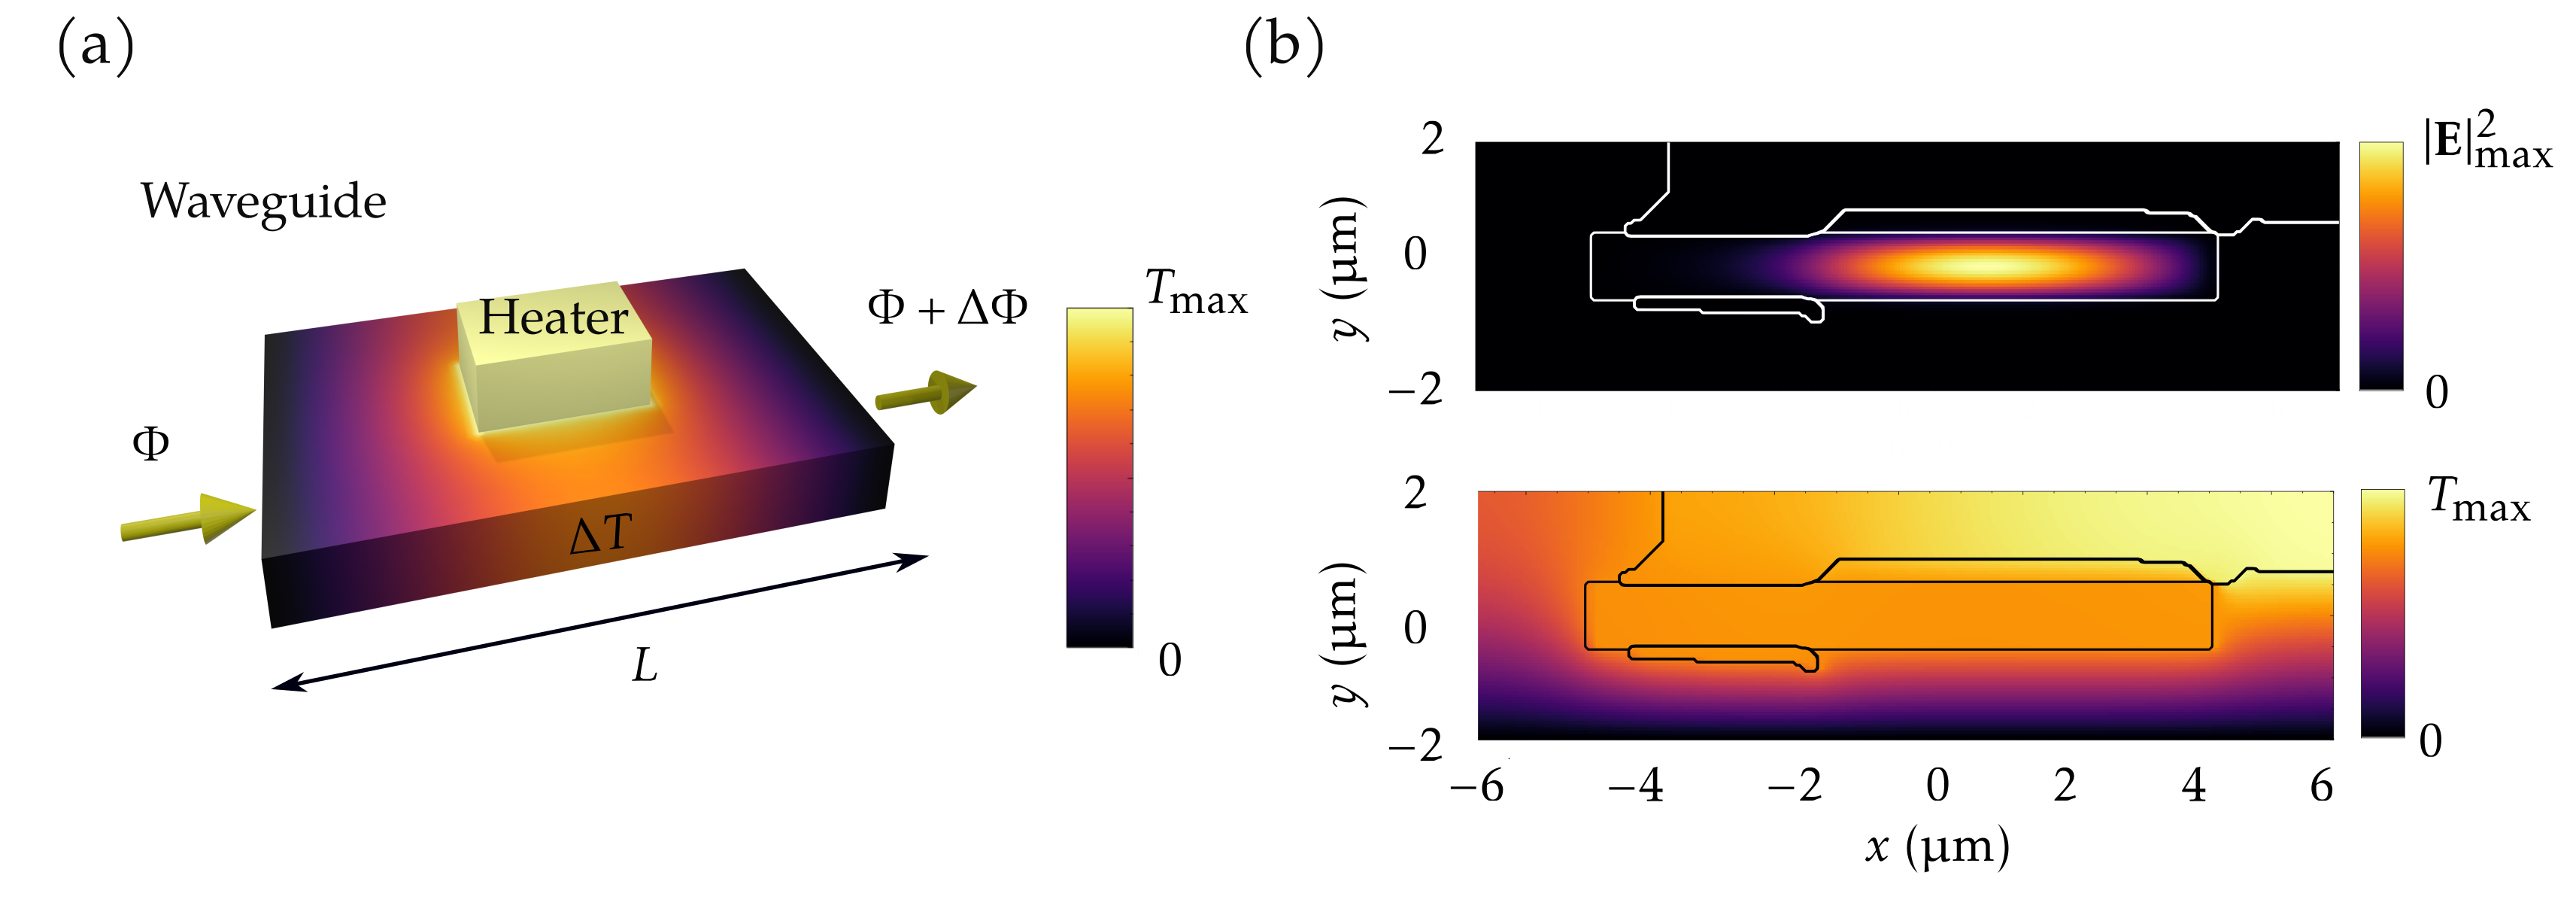
\includegraphics{figures/TOPS_results.png}}%%
    \caption{Topology optimization of thermo-optical phase shifters. (a) Phase-shifting mechanism, where a heater changes the temperature in the waveguide $\Delta T$, inducing a phase shift
    $\Delta \Phi$ over a length $L$. (b) Thermal and optical response of the topology optimized device. Figure adapted with permission from~\cite{ownpub0} © Optical Society of America.}
    \label{fig:thermo_res}
\end{figure}


\subsection*{The effective index via waveguide finite element analysis}

To calculate the phase shift (\eqref{eq:phase_shift}), one needs to find the effective index of an optical mode. This can be done by 
using the finite element formulation for two-dimensional waveguide cross-sections described in~\cite{jin}
\begin{equation}\label{eq:wg_eq}
 \left[\begin{array}{cc}
 A_{\text{tt}}(\varepsilon,k) & 0 \\
    0 & 0
    \end{array}\right]
 \left\{\begin{array}{l}
 E_{\text{t}} \\
 E_z
    \end{array}\right\}
 = -k_z^2
 \left[\begin{array}{cc}
 B_{\text{tt}} & B_{\text{t} z} \\
 B_{z \text{t}} & B_{z z}(\varepsilon,k)
    \end{array}\right]
 \left\{\begin{array}{c}
 E_{\text{t}} \\
 E_z
    \end{array}\right\},
    \end{equation}
where $E_{\text{t}}$ and $E_z$ are the transverse ($x,y$) and longitudinal ($z$) electric field components respectively, $k_z$ is the propagation constant of the optical mode, and $A_{tt}, B_{tt},
B_{zt}$, $B_{tz}$, and $B_{zz}$ are matrices that can be assembled using the shape functions (\eqref{eq:ned_shape})~\cite{jin}. Following~\cite{jin}, we use Nédélec elements (\secref{sec:fem}) for the in-plane components of the electric field and 
Lagrange elements for out-of-plane components. 

Solving the generalized eigenvalue problem in \eqref{eq:wg_eq} yields waveguide modes ($E_t$, $E_z$) and propagation constants ($k_z$). The propagation constant can be rewritten into the \textbf{effective index} $n_\text{eff} = k_z / k$,
 where the real part is a measure of the mode overlap with the refractive index distribution, and the imaginary part ($\Im\{n_\text{eff}\}$) quantifies modal losses. For a numerical implementation of this method, please refer to our GitHub repository~\cite{FEWEC}, which includes a tutorial on solving the 
 generalized eigenvalue problem in \eqref{eq:wg_eq} to find the effective indices and field distributions of waveguide eigenmodes.

 \subsection*{PT-symmetry breaking waveguides}
 Recent progress in waveguide design by Dave and Lipson~\cite{lipson}, proposed the use of \textbf{PT-symmetry breaking} (\secref{sec:nanophotonics}) \textbf{waveguides} as promising candidates for
 thermo-optical phase shifter devices, since they can minimize optical losses while being placed in close contact with (lossy) metallic heaters. To understand this phenomenon, we consider an example with a 
 simulation domain with a $5$ \textmu m height and a $15$ \textmu m width. At the center of a silica cladding ($n\approx 2$) there is a silicon ($n \approx 3.48$) waveguide with a $2$ \textmu m height and 
 a $10$ \textmu m width, where the left half ($x<0$) of the waveguide is lossy [characterized by an extinction coefficient $\kappa>0$ (\eqref{eq:perm})].

\begin{figure}[tb]
    \centering
    \makebox[\textwidth][c]{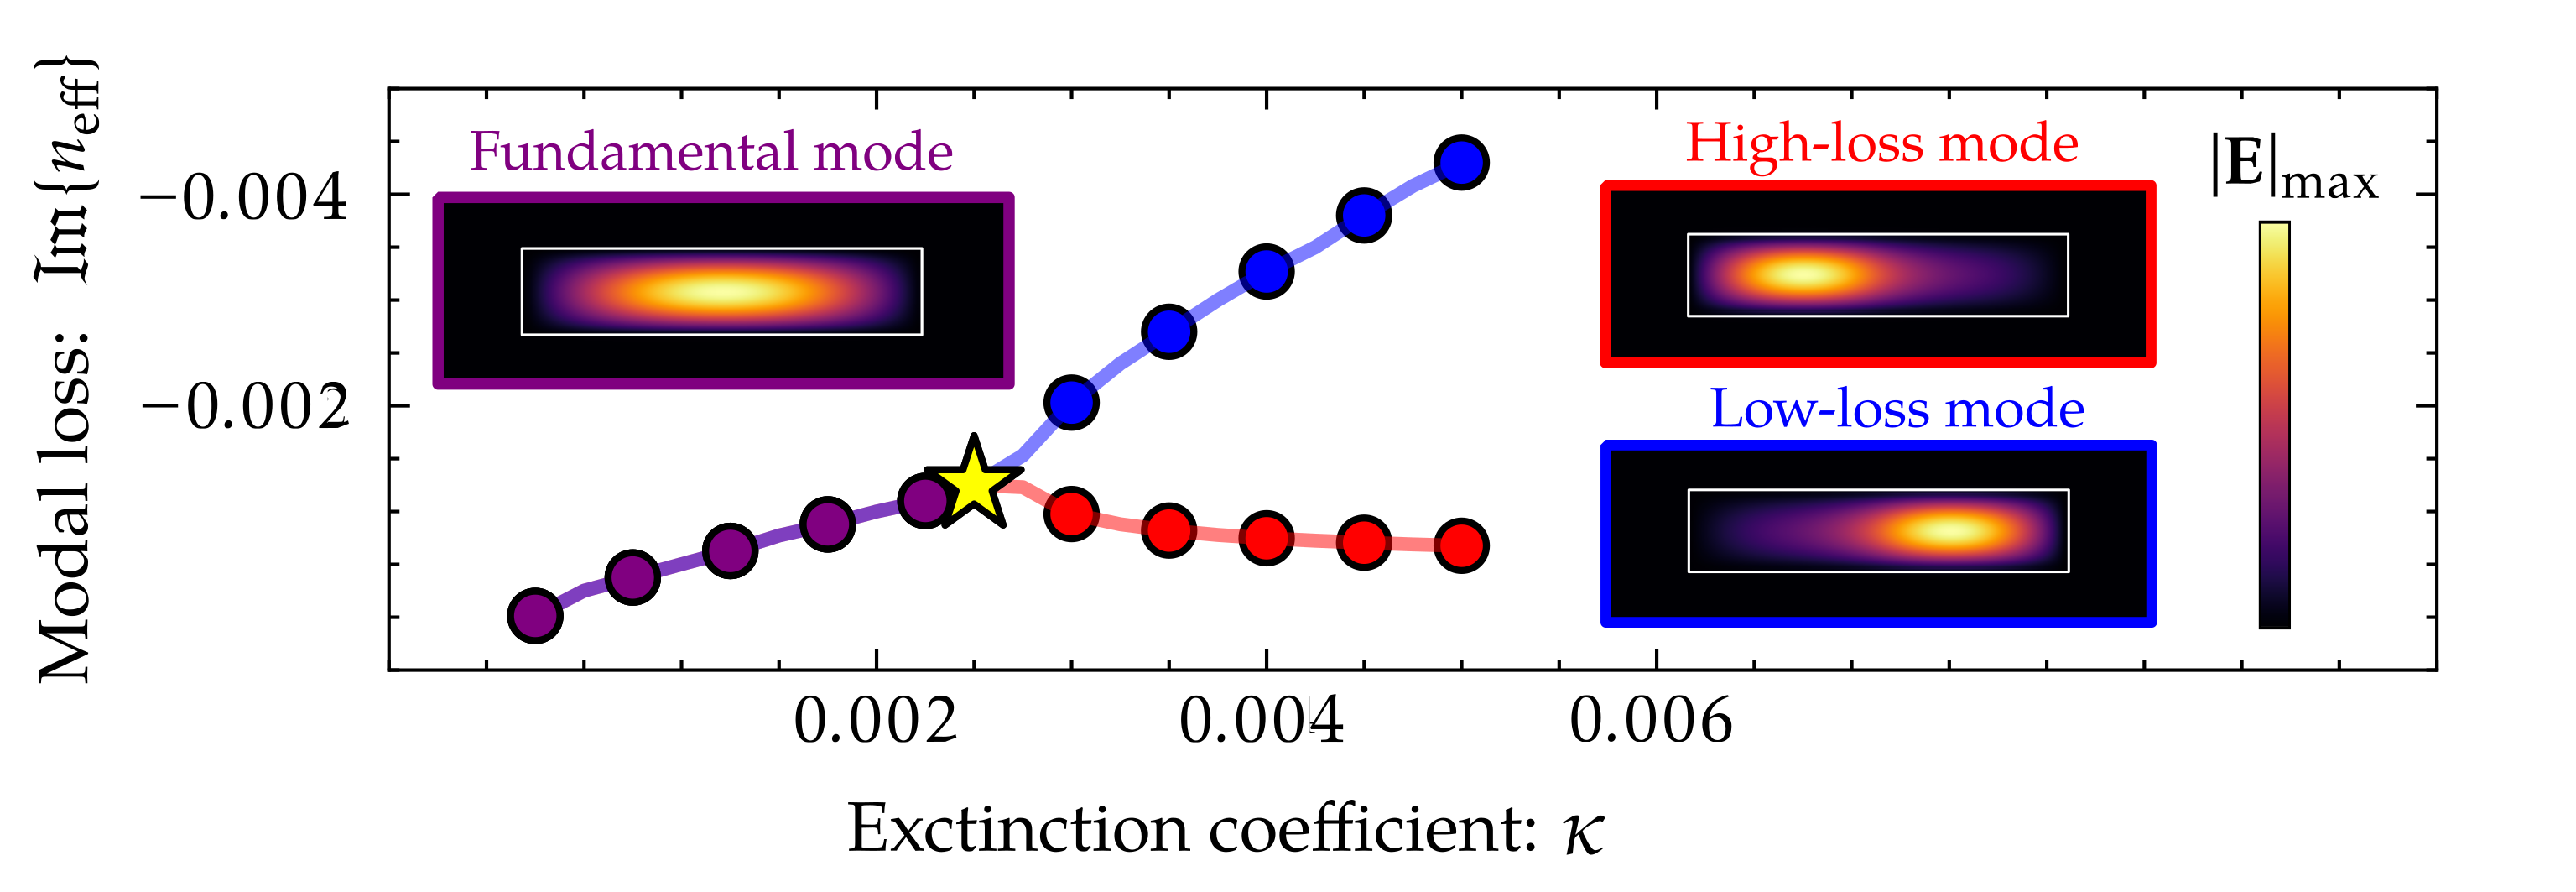
\includegraphics{figures/TOPS_pt.png}}%%
    \caption{Parity-time symmetry breaking mechanism in lossy waveguide modes. The modal losses ($\Im\{n_\text{eff}\}$) as a function of the extinction coefficient ($\kappa$) show the splitting of the fundamental mode into 
    high- and low-loss modes, with their max-normalized electric field norm ($\vert \mathbf{E} \vert$) distribution.}
    \label{fig:pt}
\end{figure}

Using this configuration and perfect electric conductor boundary conditions, we solve the eigenproblem in~\eqref{eq:wg_eq} at the telecom wavelength ($\lambda = 1.55$ \textmu m) for varying extinction coefficients. 
 As shown in~\figref{fig:pt}, increasing the extinction coefficient initially makes the fundamental mode more lossy until a bifurcation (star in~\figref{fig:pt}) splits
  it into high- and low-loss modes. Counter-intuitively, further increasing the extinction coefficient reduces the loss of the low-loss mode 
  because its spatial profile overlaps more strongly with the lossless half of the waveguide.
   This effect is beneficial in thermo-optical waveguide design, since it enables placing a metallic heater in direct contact with the waveguide for better heat transfer while still
    maintaining low optical losses.

\subsection*{Topology optimization results~\cite{ownpub0}}

Inspired by PT-symmetry breaking waveguides, in~\cite{ownpub0}, we use topology optimization to achieve good heat conduction and low optical loss in thermo-optical phase shifters.
The optimization problem considers a waveguide cross-section with a lossy metallic heater, and seeks to find the distribution of metal around the waveguide that minimizes optical loss for both heated and 
unheated configurations. 

Unlike the eigenvalue-based approach presented in the previous section, which estimates losses from the imaginary part of the effective index,
 our method evaluates losses by directly solving a linear system. An optical source excites the waveguide mode, which appears
  as a resonance in the effective index spectrum. The imaginary part of the refractive index ($\Im\{n_\text{eff}\}$) represents the resonance linewidth and therefore the loss:
   the smaller it is, the sharper the resonance and the lower the loss. By maximizing the electric field intensity of the excited mode,
    we can sharpen this resonance and thus minimize losses. Based on this idea, we formulate an optimization problem that designs
     the metallic heater around the waveguide by maximizing the worst-case electric field intensity at two effective indices, representing
      the heated and unheated waveguide states. An example of this is shown in \figref{fig:therm_opt_neff}, where we plot the maximum electric field intensity in the waveguide as a function of 
      the effective index for the optimized device (\figref{fig:thermo_res}) and a reference design in the unheated and heated configurations, showing larger and sharper resonances 
      for the optimized device.
 
      \begin{figure}[b]
         \centering
         \makebox[\textwidth][c]{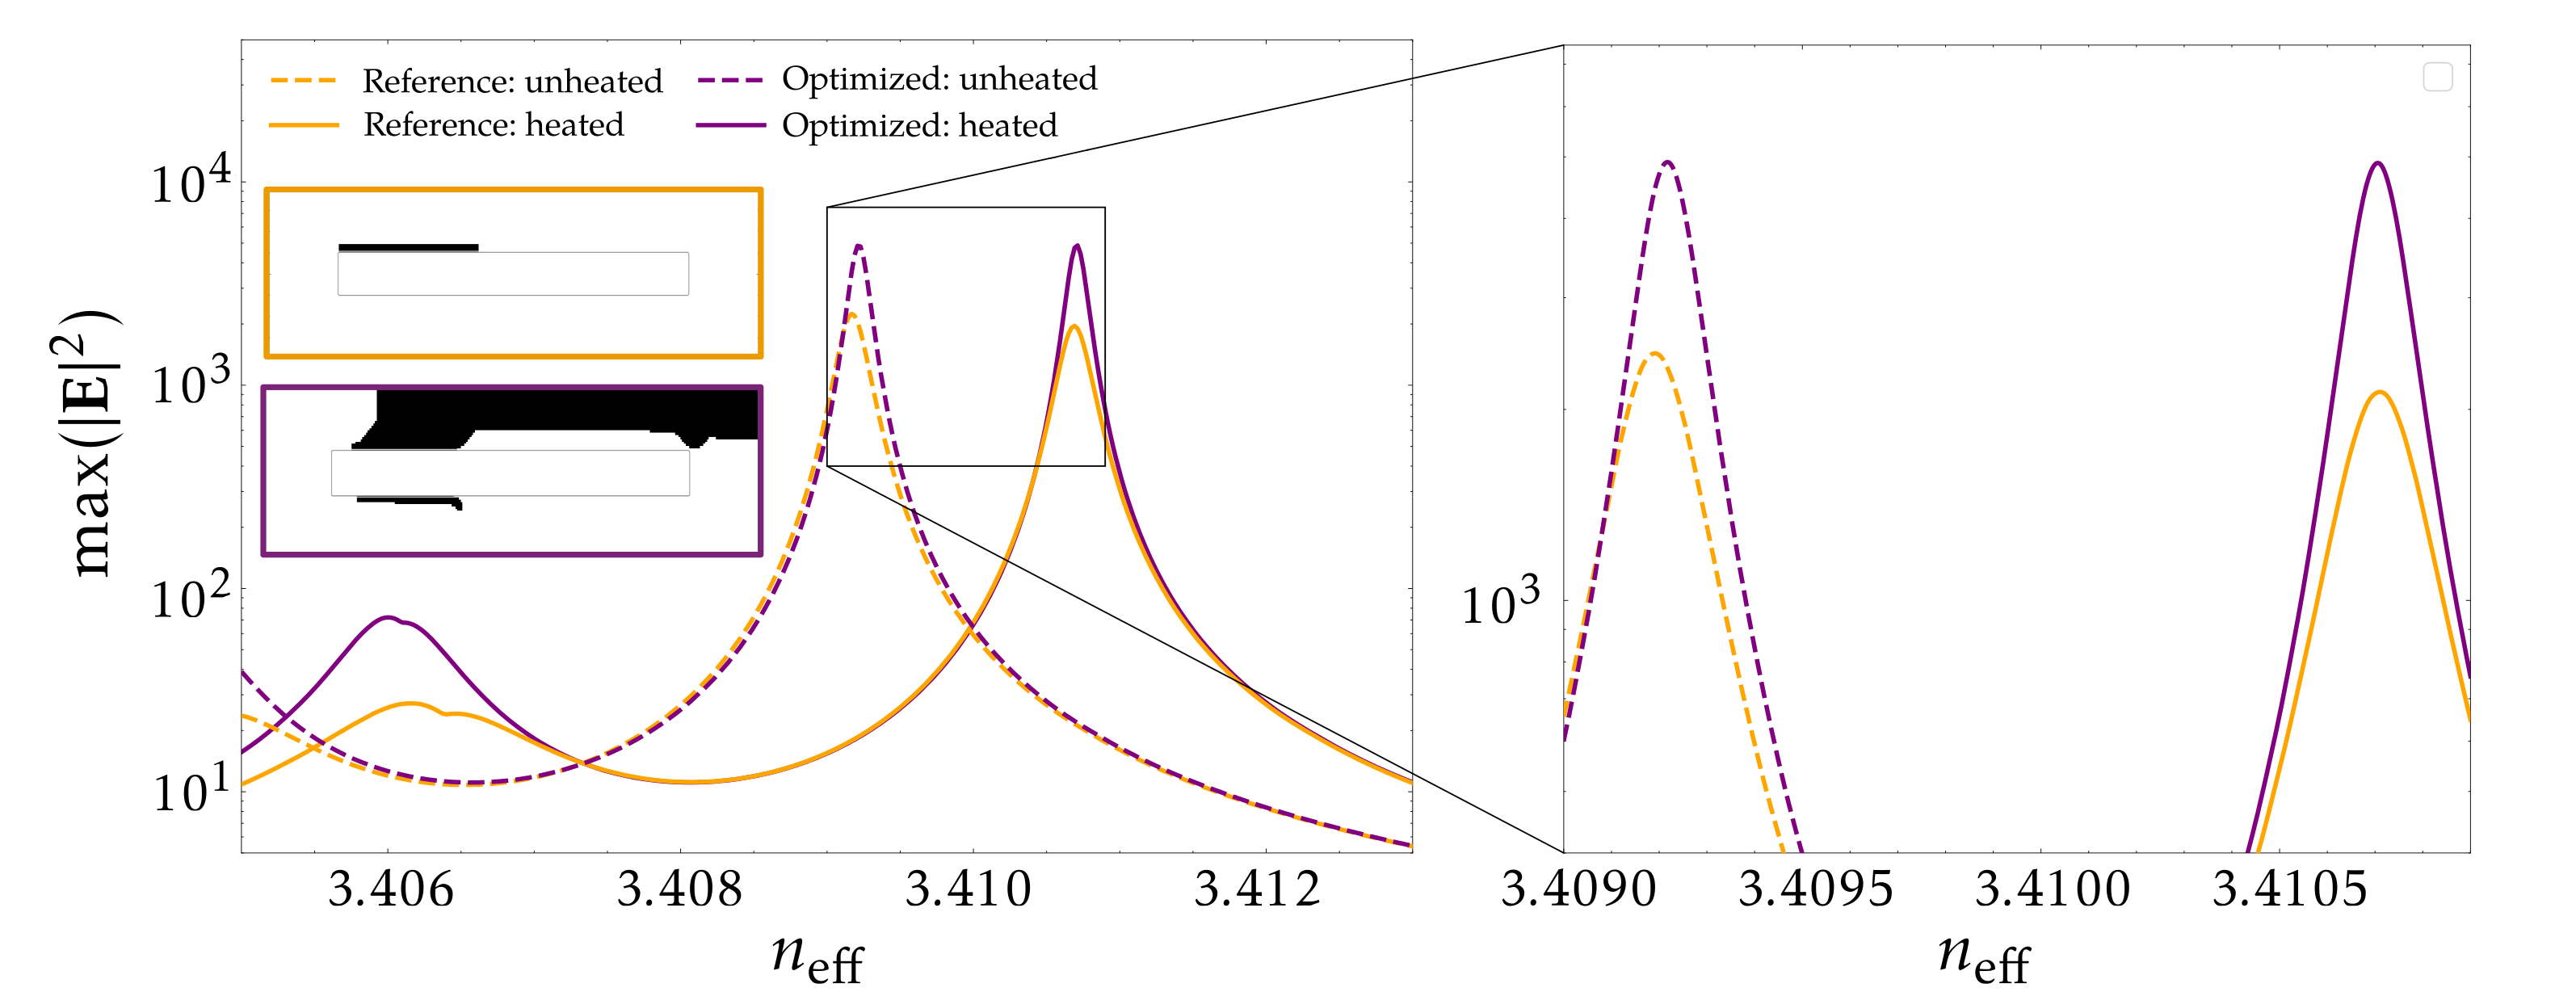
\includegraphics{figures/TOPS_results_2.png}}%%
         \caption{Maximum electric field intensity [$\max(\vert \mathbf{E} \vert^2)$] in the waveguide as a function of the effective index for the topology-optimized and reference designs in the unheated and heated
         configurations. Figure adapted with permission from~\cite{ownpub0} © Optical Society of America.}
         \label{fig:therm_opt_neff}
      \end{figure}
      

 To integrate the heat problem into the 
 topology optimization framework, we use a linear material interpolation 
for the conductivity (Eq. 13 in~\cite{ownpub0}) and an interpolation for the heat source given by $
 Q(\hat{\rho})=P_{\text{in}} \hat{\rho}^p / \left( L A_e \sum^{N_\text{e}}_j \hat{\rho}_j \right)\,,
$
where $P_\text{in}$ is the input power in the heater, $p$ is a penalization factor, $A_e$ is the area of each element, and 
$N_e$ is the total number of elements in the finite element problem. 
This expression models a resistive heater with all material connected in parallel, so that for a fixed input power, the heat 
generation per unit volume increases as the total heater volume decreases.
To solve the inverse design
problem, we derive a coupled adjoint sensitivity analysis~\cite{ownpub0} enabling gradient-based optimization.

Using this framework, we find the results in \figref{fig:therm_opt_neff} and \figref{fig:thermo_res} (b), where we depict the waveguide cross-section with the topology-optimized metallic heater,
allowing the same low-loss mode to propagate in both the heated and unheated scenarios,
reducing optical losses by $\approx 33 \%$ compared to state-of-the-art PT-symmetry breaking thermo-optical phase-shifter proposals (see reference design in \figref{fig:therm_opt_neff})~\cite{lipson}. Similar to the devices
in~\cite{lipson}, the optimized design utilizes the spatially heterogeneous loss profile to engineer an efficient low-loss mode. Using this optimized device as a starting point, several extensions of the topology optimization problem are considered in~\cite{ownpub0}, such as varying volume constraints, optical power, and the inclusion of fabrication constraints (e.g., minimum length scales and layered 
lithography processes).

\subsection*{Outlook and future work}

The framework presented in our work~\cite{ownpub0} provides a foundation for studying and optimizing weakly coupled topology optimization problems. For example, for the design of phase shifters and thermo-optical modulators, it should be straightforward to extend this
formalism to three dimensional system, where one could account for insertion/coupling losses of the integrated photonic circuits. Another example is the use of multi-material topology optimization to design the heating device and the optical waveguide simultaneously. Moreover, this formalism could be applied to design completely different devices, such as re-configurable photonic systems that might be modulated by an external heat source, or thermo-optical
switches based on optical cavities~\cite{switch, switch_2}, where the change in refractive index shifts the cavity in- or out-of-resonance. Lastly, the thermo-optical phase-shifter problem could be
extended to electro-optical phase shifters~\cite{pockels} (\secref{chap:eo}), since the electrostatic Poisson equation $\nabla^2 \phi = -\rho/\varepsilon_0$ is a special case of the heat equation with a spatially homogenous
conduction coefficient, where $\phi$ is the electric potential that replaces the temperature profile. 

\section{Towards strong coupling -- heat dissipation in optics}\label{sec:thermo_strong_coupling}

In the strong coupling regime, the optical response will modify the thermal response, and vice versa.
An example of such an effect is \textbf{optical absorption}, which can lead to significant local heating, altering the refractive index and thus modifying the optical field. 
This mutual dependence requires a strongly coupled treatment of the heat and optical problems (\secref{sec:coupled}), modeled via an electric-field-dependent volumetric heat source~\cite{plasm_heat_source}
\[
Q(\mathbf{r}) = \frac{1}{2} \omega \varepsilon_0 \varepsilon_r^{\prime \prime} |\mathbf{E}(\mathbf{r})|^2,
\]
where the material losses ($\varepsilon_r^{\prime \prime}$) convert the electromagnetic energy into heat. 
This expression is critical for metal nanostructures, where plasmonic resonances cause localized heating~\cite{plasm_heat_source}, and in high-intensity photonics, where even weakly absorbing materials can produce significant heat~\cite{thermal_nl, high_I_T}. Moreover, the thermo-optical feedback can give rise to nonlinear effects (\secref{sec:nanophotonics}), such as self-focusing~\cite{thermal_nl}. If we still consider a linear
thermal response and TOC,
the nonlinearity has the form of a Kerr-type nonlinearity ($\Delta n \propto \vert \mathbf{E} \vert^2$). Accounting for and modeling
these effects could open up the avenue for the inverse design of novel nonlinear thermo-optical devices, with potential applications
in integrated nonlinear photonics~\cite{nl_photonics}, metasurfaces~\cite{nl_meta}, and plasmonics~\cite{novotny}.

\section{Heat transfer as a connectivity constraint}\label{sec:aux}

Lastly, it is worth mentioning that an additional heat equation can be used as an auxiliary equation to enforce connectivity
and structural integrity in topology optimization problems (e.g.,~\cite{vanessa, structural_heat}), which is also exemplified by some of our
works~\cite{ownpub1,ownpub2}. 

This method, introduced in~\cite{li_structural_2016}, is known as the \textbf{virtual temperature method} (VTM). The core idea of the VTM is to simulate a heat transfer problem on an auxiliary thermal field, where the solid domain
 is treated as a heat source and a thermally conductive material. At the same time, void regions are modeled as an
insulating material, and Dirichlet boundary conditions ($T = 0$) are imposed on the boundaries where connectivity is required, while Neuman boundary conditions are imposed
on the rest of boundaries. When 
solving the steady-state heat equation (\eqref{eq:heat}), regions that are disconnected from the boundary 
cannot dissipate heat and therefore attain elevated temperatures. By applying a threshold criterion on the thermal field, such as $T < T_\text{thresh}$, disconnected islands in the design can be 
detected and penalized. For instance, in our works~\cite{ownpub1,ownpub2}, we compute a measure of the total virtual temperature
by integrating the temperature field over the design domain ($\Omega_D$), and add it as a constraint in the optimization problem 
$\int_{\Omega_D} T \d \Omega \leq \epsilon_C$, where $\epsilon_c$ is a sufficiently small constant. Accounting for this constraint in the optimization problem ensures that the final design remains physically connected to the required 
boundaries. 


Note that by appropriately selecting the connecting boundaries it is possible to use the VTM to enforce
(mechanical) structural integrity of the designs~\cite{structural_heat}, which can also be achieved by solving an auxiliary
mechanical problem~\cite{structural_integrity}. For a more robust connectivity constraint formulation with less parameter tuning, we refer the reader to the nonlinear 
virtual temperature method (NVTM)~\cite{nvtm}, and for further details on connectivity constraints, we refer the reader to the review 
article by Cool et al.~\cite{vanessa}.

\openright
\chapter{Optomechanical topology optimization problems}\label{chap:om}
%\section{Opto-mechanical systems~\cite{ownpub1,ownpub2,ownpub3}}\label{sec:optomechanics}
Optomechanics, the study of the interaction between light and mechanical motion, is at the heart of state-of-the-art technologies, such as 
optical trapping~\cite{ashkin_acceleration_1970, moffitt_recent_2008} and cooling~\cite{cooling}, quantum information processing~\cite{Andrews_2014, Xi_2025}
, light sails~\cite{lightsail, lightsail1}, and high-precision metrology and sensing~\cite{sensing, weakforce, Li:18, Mason_2019}. The most basic description of this interaction is given by the \textbf{Lorentz force}, which governs how moving charges respond to electric and magnetic fields:
\begin{equation}\label{eq:lorentz_f}
    \mathbf{\mathbf{F}}(\mathbf{r},t) = q \left[ \bm{\mathcal{E}}(\mathbf{r},t) + \mathbf{v}(t) \times \bm{\mathcal{B}}(\mathbf{r},t) \right]\,,
\end{equation}
where $q$ is the charge and $\mathbf{v}$ is the velocity of the particle. This force can be generalized to describe more complex systems,
such as the the force between two current-carrying 
wires (Ampere's force law), and the electromotive force, which is at the core of many techologies, such as induction motors or generators.
In optomechanical systems, shaping the distribution and magnitude of these forces at the micro- and nanoscale is crucial for controlling mechanical motion with light. 
However, designing structures that can efficiently harness and manipulate these interactions often requires navigating highly complex
 parameter spaces and trade-offs between optical, mechanical, and material constraints.

 One effective approach for enhancing and shaping optomechanical interactions is to use topology optimization.
Recent advances in optomechanical topology optimization include the design of coupling between optical and elastic
 waves~\cite{photo_topopt}, optical systems with nonlinear deformations~\cite{def_wg}, high-$Q$ optomechanical membranes~\cite{highQ1, fengwen, aragon1},
light sail structures~\cite{lightsail_topopt, lightsail_topopt1},
on-chip optical trapping devices~\cite{ownpub1}, particle design and manipulation~\cite{ownpub2, particle_opt},
and structural integrity constraint formulations~\cite{structural_integrity}
 among others.

 In the following subsections, we highlight our contributions to the field and review how to model optomechanical interactions in three distinct regimes: a general treatment based on the Maxwell stress tensor~\cite{ownpub2}; 
 the dipole approximation in the small particle limit~\cite{ownpub1, ownpub3}; and strongly coupled systems where optical forces can induce significant mechanical deformations.
\section{The Maxwell Stress Tensor formalism~\cite{ownpub2}}\label{sec:engi}

In the most-general case, the optical force can be calculated using the \textbf{Maxwell stress tensor} (MST) formalism, which is a generalization of the Lorentz force (\eqref{eq:lorentz_f}) in continuous media~\cite{novotny}.
The basic idea is sketched in \figref{fig:eng_res}, where
a particle scatters an incident time-harmonic electromagnetic field $\mathbf{E}_\text{inc}$ creating the time-harmonic scattered field $\mathbf{E}_\text{scat}$ and the net force $\mathbf{F}$ that acts
on the particle. The time-averaged net force is given by~\cite{novotny}
\begin{equation}\label{eq:f_MST}
    \mathbf{F} \equiv \langle\mathbf{F}\rangle=\int_{\partial V}\langle\stackrel{\leftrightarrow}{\bm{\mathcal{T}}}(\mathbf{r}, t)\rangle \cdot \mathbf{n}_{\partial V}(\mathbf{r}) \d \mathbf{r}\,,
\end{equation}
where $\partial V$ denotes any boundary enclosing the particle, $n_{\partial V}$ denotes the unitary vector normal to that boundary, and
the time-average of the stress tensor is given by
\begin{equation}
        \langle \stackrel{\leftrightarrow}{\mathbf{T}}(\mathbf{r}, t) \rangle 
        = \frac{1}{2} \Re \Big\{ 
            \varepsilon\, \mathbf{E}(\mathbf{r}) \otimes \mathbf{E}^*(\mathbf{r})
            + \mu\, \mathbf{H}(\mathbf{r}) \otimes \mathbf{H}^*(\mathbf{r})
         - \frac{1}{2} \big( \varepsilon\, |\mathbf{E}(\mathbf{r})|^2 + \mu\, |\mathbf{H}(\mathbf{r})|^2 \big) 
        \stackrel{\leftrightarrow}{\mathbf{I}} \Big\}.
\end{equation}
where $\otimes$ denotes the outer product. Note that the permittivity ($\varepsilon$) and permeability ($\mu$) correspond to those of the medium surrounding the particle.

\begin{figure}[tb]
    \centering
    \makebox[\textwidth][c]{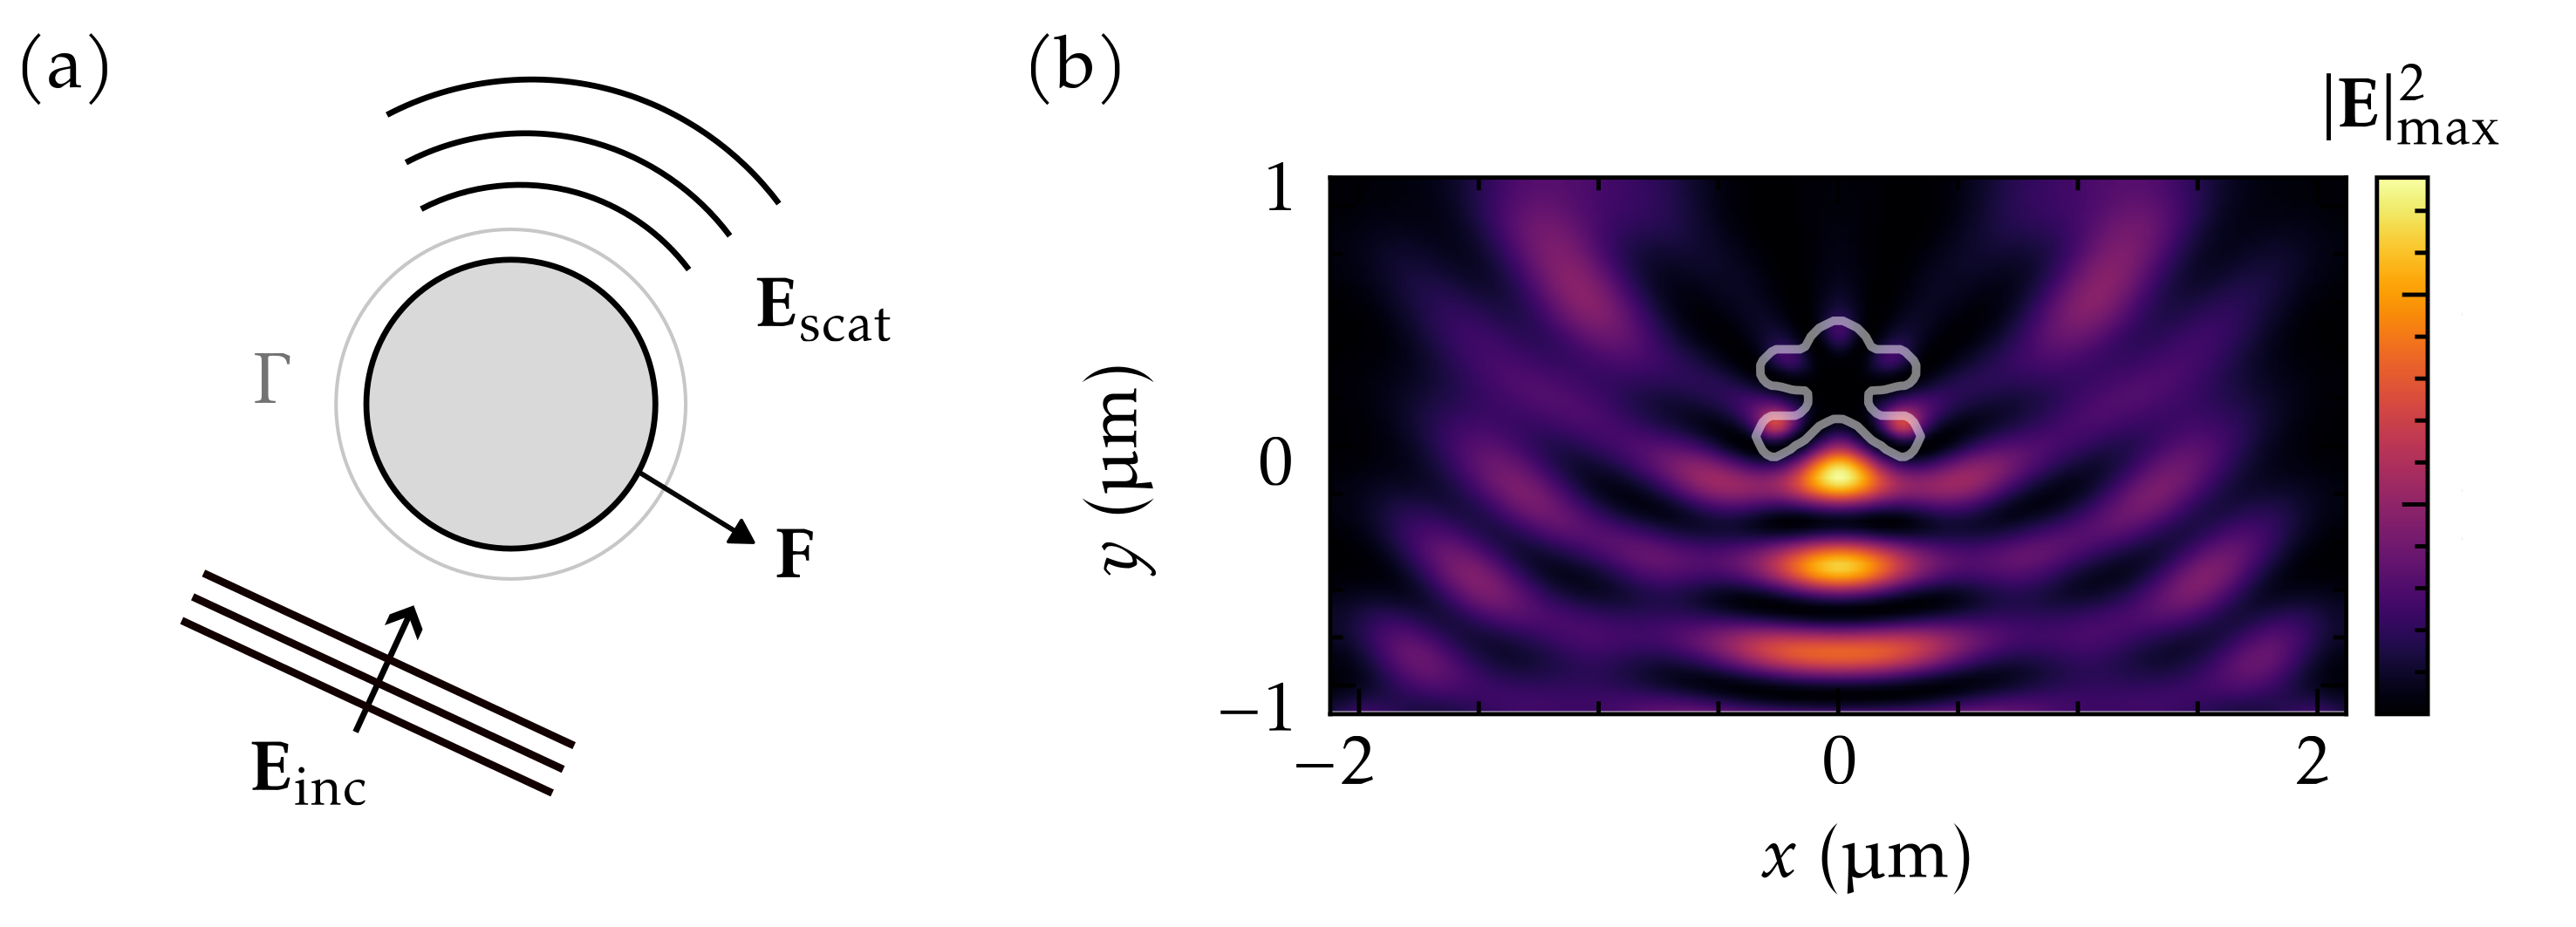
\includegraphics{figures/eng_results.png}}%%
    \caption{Topology optimization in optical force applications. (a) A scattering particle 
    enclosed by a boundary $\partial V$ scatters a field $\mathbf{E}_\text{scat}$, when excited by an incident field $\mathbf{E}_\text{inc}$, 
    generating a net optical force $\mathbf{F}$. (b) Electric-field intensity distribution for a particle design optimized to maximize the vertical ($y$)
    component of the optical force. Adapted with permission from~\cite{ownpub2} \copyright Optical Society of America.}
    \label{fig:eng_res}
\end{figure}

\subsection*{Engineering optical forces via topology optimization}

In~\cite{ownpub2} we apply this formalism to optimize the geometry of particle-metalens pairs for difference applications, such as attracting, repelling, 
oscillating and trapping particles. In \figref{fig:eng_res} we depict an example optimization result from our work, where 
we optimize the geometry of a particle to maximize the vertical component of the optical force by targeting $\text{FOM} = \langle\mathbf{F}\rangle \cdot \mathbf{n}_y$, where
in our two-dimensional example $\mathbf{n}_y = (0, 1)$ is the unitary vector in the vertical direction.  Our results show that the optimized particle geometry is a Bragg-mirror-like
structure, which is able to efficiently reflecting the incoming plane-wave, resulting in a efficient exchange of force and momentum. As a matter of fact, by comparing the response of the optimized design
to a reference square particle, we observe that the topology-optimized device feels a $\approx 3\times$ stronger vertical force than the reference.
 Moreover, in~\cite{ownpub2} we show that by also designing a metalens to focus the incoming plane-wave onto the particle one can use nearly all the momentum available in the simulation domain\footnote{This is based on the radiation pressure force on an perfectly reflecting surface spanning the entire simulation domain~\cite{ownpub2}.} 
 to generate a net force on the particle, allowing for a $\approx 13\times$ stronger force than the reference square particle. 
 In the remainder of~\cite{ownpub2} we further extend these examples by also designing
attractive particle geometries, and optical-tweezer like setups to trap the particle in space. All the code developed in this work is available on GitHub~\cite{github_MST} with tutorials on force calculation and topology optimization. 

One interesting aspect of the topology optimization of particles in the MST formalism is that with our current framework the particle cannot feature disconnected members; otherwise,
one would need to integrate around the individual components to calculate the total force for each one. It is possible solving this problem by enforcing 
a connectivity constraint via the VTM~\cite{li_structural_2016} (see \secref{sec:aux}). In our examples
we enforce particle connectivity to the center of the particle, and connect the metalens structure to the bottom, as to ensure structural
integrity of the structure.

\subsection*{Outlook and future work}

This topology optimization work is the first, to our knowledge, to 
target optical forces via the MST formalism, paving the way for future work in three-dimensional systems and more complex optimization problems, such as optically-driven particle
trajectory control~\cite{zemanek_perspective_2019, macdonald_microfluidic_2003, shilkin_directional_2017}, many-body particle systems~\cite{bechinger_active_2016, chang_colloquium_2018} or optically actuated devices~\cite{ivanyi_optically_2024}, among others.
Finally, it is worth noting that a particularly interesting and straightforward extension of the framework would be to use the MST formalism to calculate the time-averaged torque acting on a particle, defined as~\cite{novotny}
\begin{equation}\label{eq:torque}
    \langle \bm{\tau} \rangle = \langle \mathbf{r} \times \mathbf{F} \rangle = \int_{\partial V} \langle \mathbf{r}
     \times \stackrel{\leftrightarrow}{\bm{\mathcal{T}}} \rangle \cdot \mathbf{n}_{\partial V} \d\mathbf{r} 
\end{equation}
where $\mathbf{r}$ is the vector defimed between the rotation axis and force application point. This definition of torque accounts
for two kinds of rotational motion; \textit{spinning} ($\langle \bm{\tau}_S \rangle$), where the particle rotates around its center of mass,
and \textit{orbiting} ($\langle \bm{\tau}_O \rangle$), where the particle rotates around an external axis, so that the total torque is the sum
of both the spin and orbital torque $\langle \bm{\tau} \rangle = \langle \bm{\tau}_S \rangle + \langle \bm{\tau}_O \rangle$~\cite{torque}.  Defining
and optical torque-based FOM could open the door for the design of efficient optical and biological micro- and nanomachines~\cite{rotating, gluck}.

\section{The dipole approximation~\cite{ownpub1, ownpub3}}\label{sec:dip}

When particles are much smaller than the wavelength of the electromagnetic field ($s\ll \lambda$), it is possible to model the optical force via the dipole approximation in the
quasistatic limit (see \secref{sec:nanophotonics}). In this approximation, the particle is treated as a point dipole with a polarizability $\alpha$, which describes how the particle responds to the local electric field frequency-domain $\mathbf{E}$.
In the dipole approximation the optical force on the particle can be expressed as~\cite{novotny}:
\begin{equation}\label{eq:dip_force}
    \langle\mathbf{F}\rangle=\overbrace{\frac{\alpha^{\prime}}{4} \nabla\left\{\mathbf{E}^* \cdot \mathbf{E}\right\}}^{(\text{G})}
    +\frac{\alpha^{\prime \prime}}{k \varepsilon_0} \Big[\overbrace{\frac{1}{c}\langle \mathbf{S} \rangle}^{(\text{RP})} + \overbrace{c \left( \nabla \times \langle \mathbf{L} \rangle \right)}^{(\text{SC})}\Big]\,,
\end{equation}
where the polarizability can be split up into the real and imaginary parts 
$\alpha=\alpha^\prime + i \alpha^{\prime \prime}$, the Poynting vector is given by $\mathbf{S} = \mathbf{E} \times \mathbf{H}$, and the time-averaged angular momentum is 
$\langle \mathbf{L} \rangle = [\varepsilon_0/(4 i \omega)](\mathbf{E} \times \mathbf{E}^*)$. 
The term associated with the electric field intensity (G) is \textbf{gradient force}, the term with the Poynting vector is the radiation pressure (RP), while the term associated 
with the angular momentum (SC) is the spin-curl force.

In the abscence of absorption effects ($\alpha^{\prime \prime}=0$), the force is totally described 
by the gradient force, which is a conservative force that can be described as the gradient 
of a potential:
\begin{equation*}
    U (\mathbf{r}) = -\frac{\alpha^{\prime}}{4} \left|\mathbf{E}(\mathbf{r})\right|^2\,.
\end{equation*}
where the force can be calculated as $\mathbf{F} = -\nabla U(\mathbf{r})$. In optical trapping applications $U$ is often referref to as the \textbf{trapping potential}.
For non-resonant and non-absorbing isotropic particles the polarizability is 
described through the relation~\cite{BornWolf:1999:Book} 
    $\alpha^{\prime}= 3 \varepsilon_0 $V$ (\varepsilon_p-\varepsilon_m)/(\varepsilon_p+2 \varepsilon_m)\,,$
where $V$ is the volume of the particle, $\varepsilon_p$ and $\varepsilon_m$ are the
dielectric constants of the particle and the medium, respectively. Note that in the dipole approximation, for infinitesimally small particles, the field $\mathbf{E}$ is not modified by the presence of the particle.
This works well for point-like particles in free-space but not necessarily 
for either large particles, particles with high refractive contrast, or particles close to material
boundaries (e.g., optical cavities). The interaction between the background field and the particle interaction can be accounted for in the dipole
approximation by considering the \textbf{self-induced back-action} (SIBA) effect, which assumes a weak
perturbation of the field due to the presence of the particle and expands the field in terms of 
the scattering Green function of the particle, which leads to a self-consistent
equation for the total electric field which can be used to calculate the force~\cite{novotny, SIBA, benjamin}. If the series converges this leads 
to same result as the MST calculation (\eqref{eq:f_MST}), which is often used to validate the dipole approximation (e.g., \cite{ownpub1,ownpub3}). 

\subsection*{On-chip omnidirectional optical trapping via topology optimization~\cite{ownpub1}}

Using the dipole approximation formalism in~\cite{ownpub1} we use topology optimization to design an integrated omnidirectional trapping optical cavity,
which was previously only possible with the use of free-space optical tweezers~\cite{ashkin_acceleration_1970}, or bulky photonic devices~\cite{manka_simulation_2024}. The trapping device
consists of two silicon waveguides connected to a central design domain, in which
topology optimization is applied (\figref{fig:MST_dipole}). The central region contains a cylindrical air exclusion with a radius
$R_\text{exc}=300$ nm and a thickness of $800$ nm, in which the stable trap is located.
To design an omnidirectional trapping device we minimize  
the difference of the electric-field norm with respect to a reference field $\mathbf{E}_\text{ref}$:
\begin{equation}
    \text{FOM} \equiv \Phi=\sqrt{\int_{\Omega}\left[\Theta_{\beta,\eta}\left(\frac{|\mathbf{E}(\mathbf{r})|}{\left|\mathbf{E}\left(\mathbf{r}_0\right)\right|}-\frac{\left|\mathbf{E}_{\text{ref}}(\mathbf{r})\right|}{\left|\mathbf{E}_{\text{ref}}\left(\mathbf{r}_0\right)\right|}\right)\right]^2} \text{~d} \Omega
    \end{equation}
where the fields are normalized with respect to the value at the center of the cavity ($\mathbf{r}_0$), and $\Theta_{\beta,\eta}$ is the smoothed Heaviside threshold (\eqref{eq:threshold}), which ensures
potentials as steep or steeper than the reference. The reference is chosen as a Gaussian trapping potential with standard deviations $\sigma_x=\sigma_y=300$ nm and $\sigma_z=400$ nm, but can be chosen to have any other form, such as a harmonic potential ($U\propto\mathbf{r}^2$).

By applying this optimization framework we obtain the topology-optimized cavity design in \figref{fig:MST_dipole}, which is able to trap particles at the center of an optical
cavity in three dimensions and has an associated Gaussian-like trapping potential, with a depth  $U<-10\, k_B T$ at room temperature ($T=300$ K) conventionally needed to overcome Brownian fluctuations~\cite{novotny}.
Note that one of the strengths of this framework is that it relies on the dipole approximation, so that
as long as the dipole approximation is valid, one can tune the input power to trap paricles of arbitrarily small sizes.

\begin{figure}[tb]
    \centering
    \makebox[\textwidth][c]{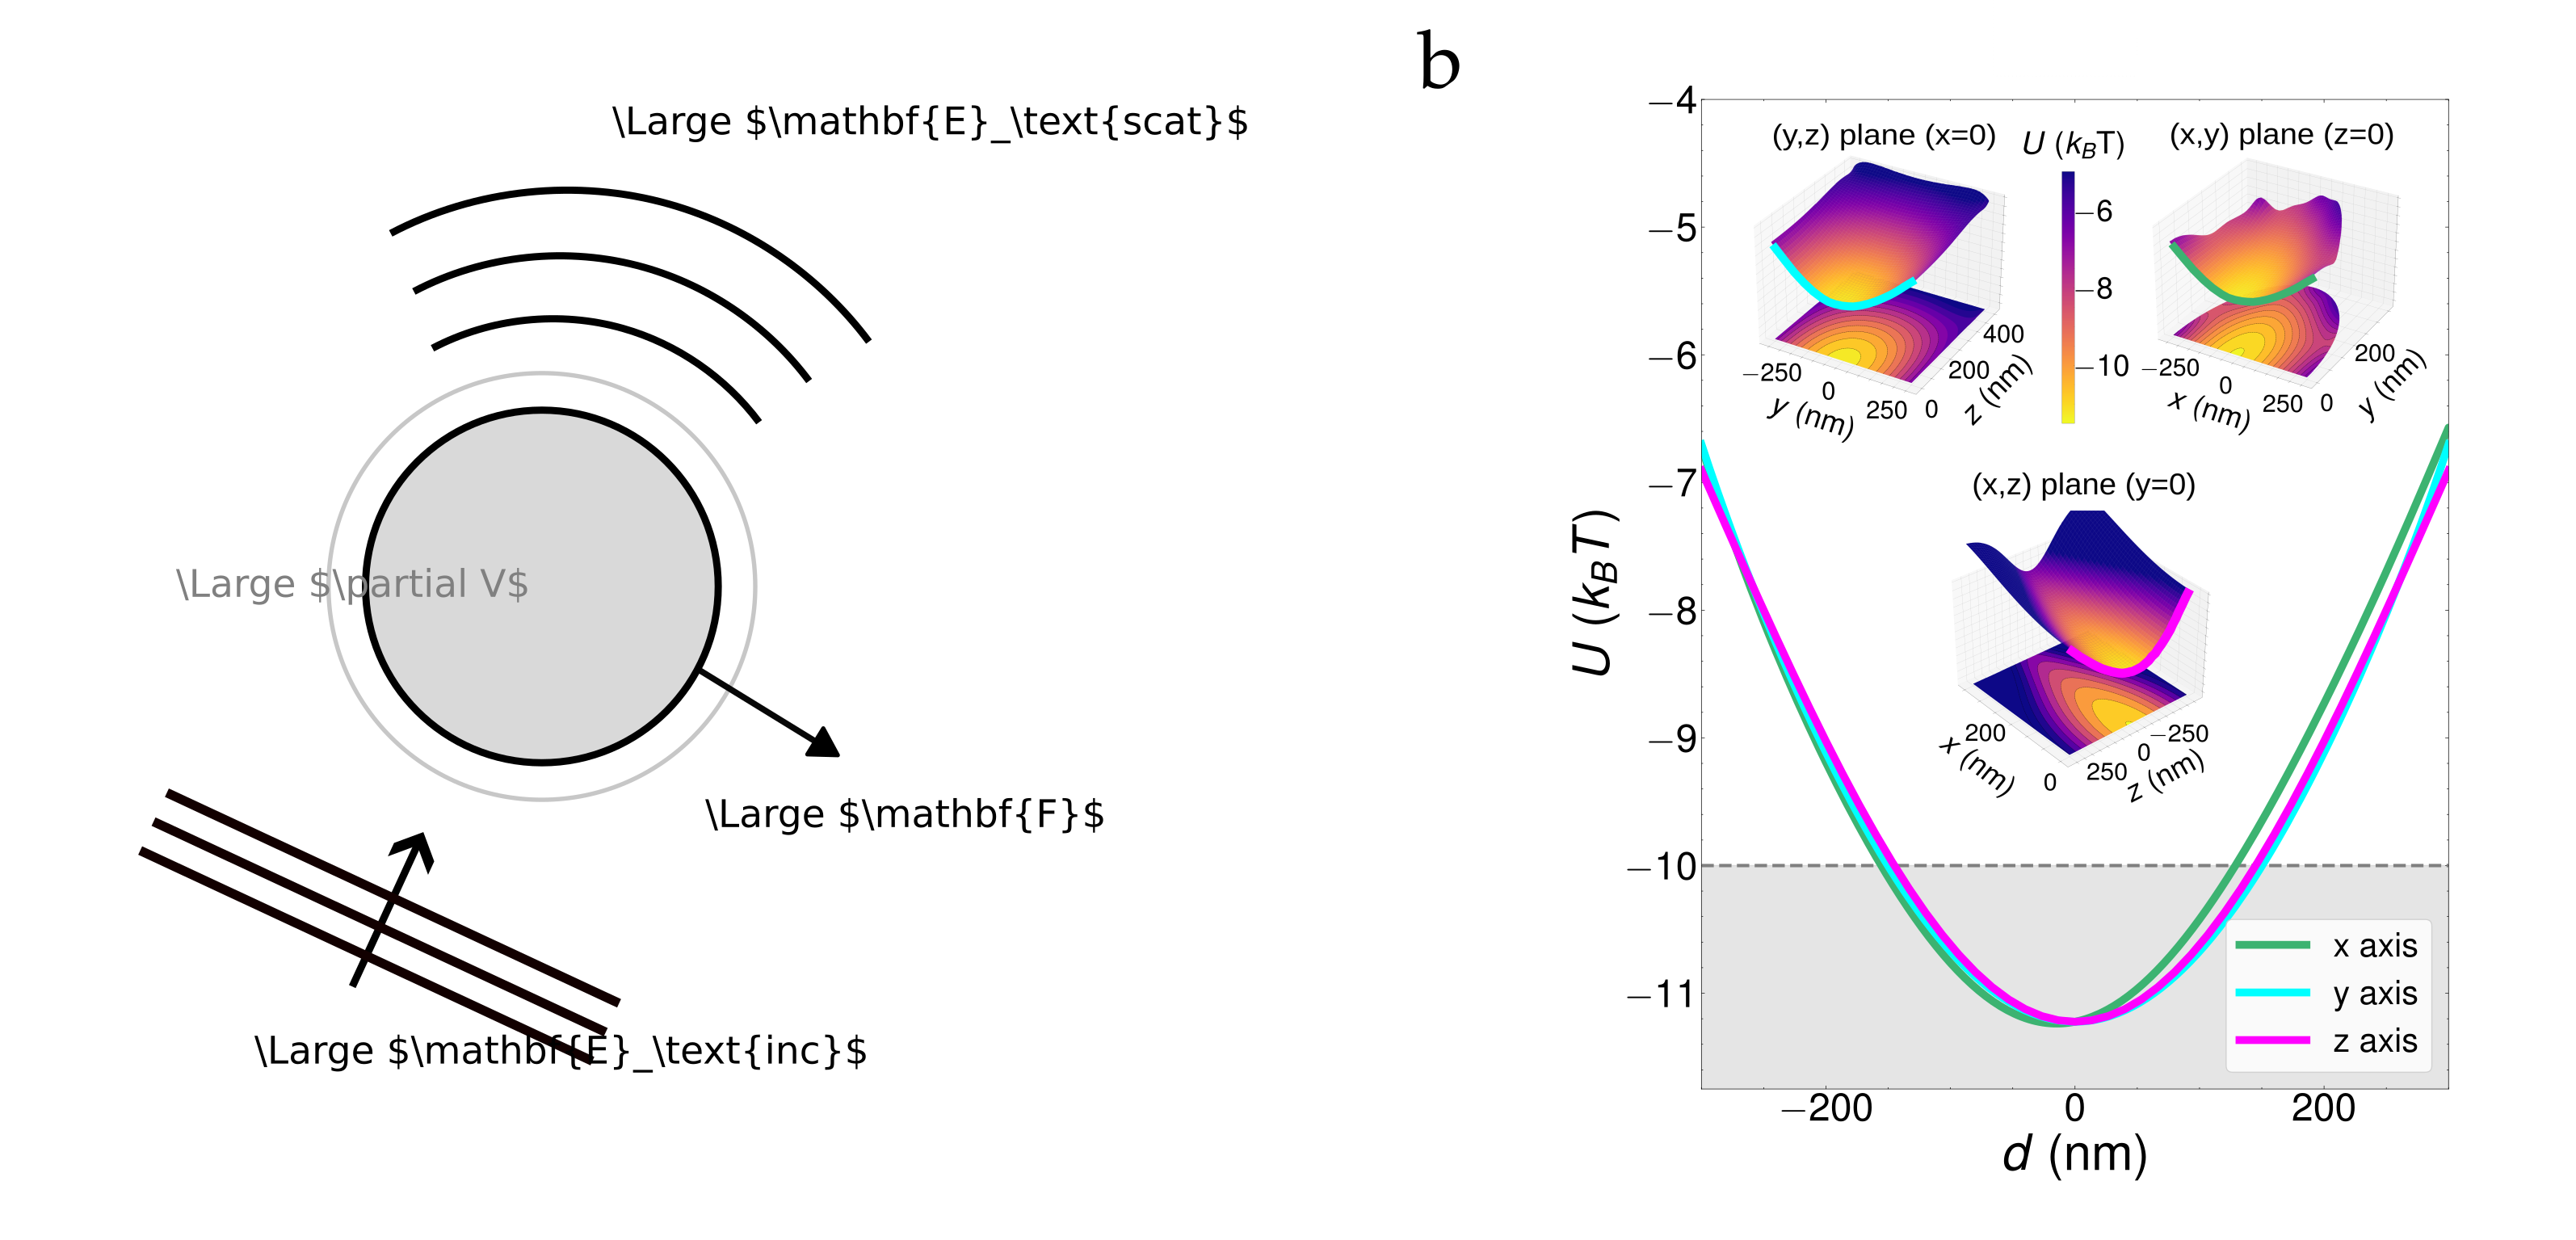
\includegraphics{figures/MST_dipole.png}}%%
    \caption{Optical response and trappig potential for the topology-optimized particle trap. (a) Lower half ($z<0$) of the optimized cavity, with the electric-field intensity
    distribution when excited with the fundamental waveguide mode at $\lambda=1.55$ \textmu m. (b) Trapping potential for a $R=15$ nm and $n=2$ particle in the cavity region for the different axial line- and plane-cuts as a function
    of the distance from the center ($d$), with the stable trapping regime ($U<-10 k_B\, T$) highlighted in gray. Adapted with permission from~\cite{ownpub1}.}
    \label{fig:MST_dipole}
\end{figure}

From the dipole approximation trapping potential we calculate the the force-displacements curves and we determine trapping stiffnesses
of $\kappa \approx 0.5$ fN/nm, an order of magnitude larger that diffraction-limited free-space optical tweezers~\cite{ownpub1}. To validate this findings
we employ the MST formalism to calculate the force on spherical particles as they are displaced from the cavity center and find excellent
agreement with the dipole approximation. As shown in \figref{fig:SPIE}, to further verify the the dipole approximation assumption, in~\cite{ownpub3} we compare the results of the dipole approximation with the MST
for varying spherical particle radii ($R_\text{sph}$) and refractive indices ($n_\text{sph}$), showing good agreement between the two methods
even for large values of the refractive index (e.g., $n_\text{sph}=3$) and particle sizes up to $s \sim R_\text{sph}\approx 0.05 \lambda$.
\begin{figure}[tb]
    \centering
    \makebox[\textwidth][c]{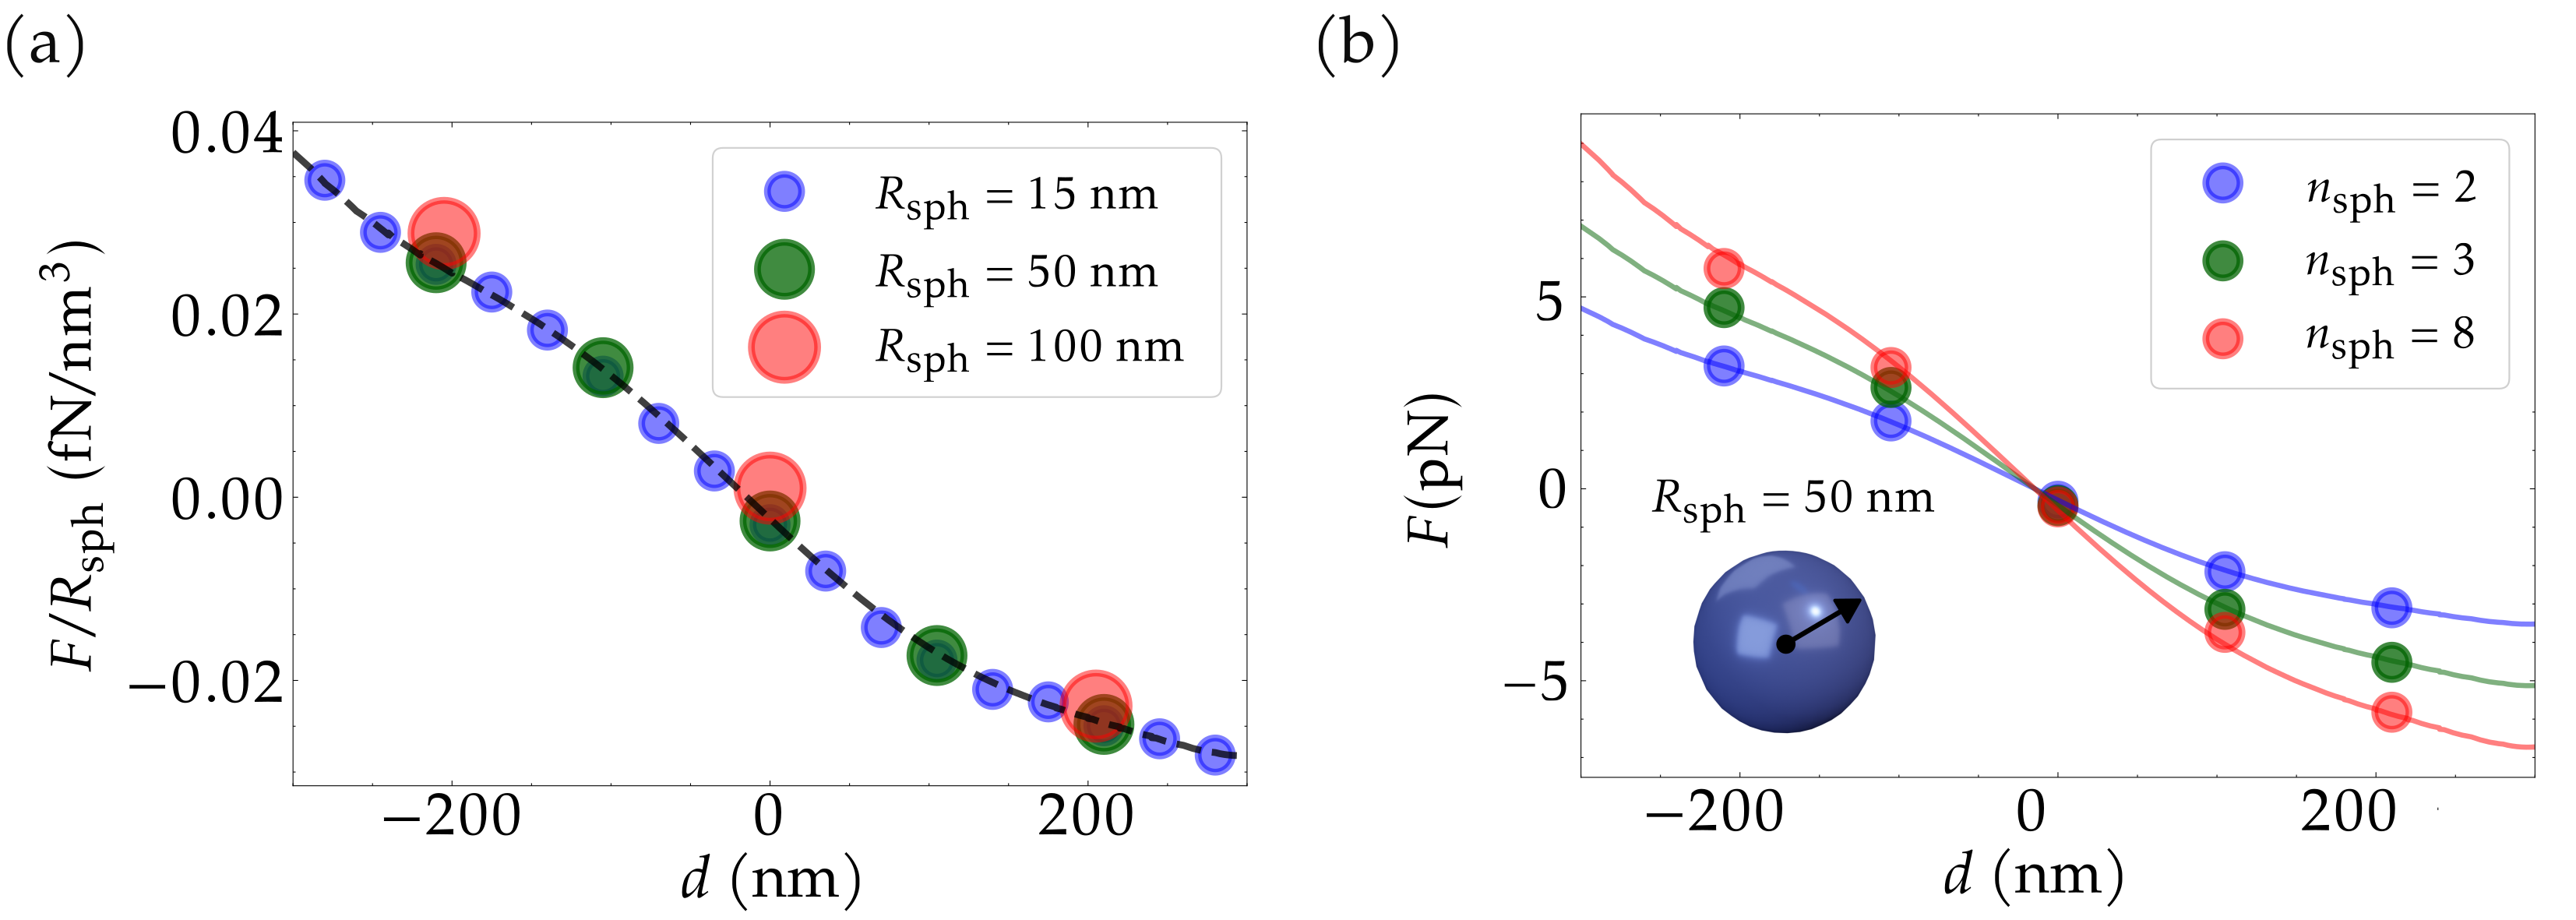
\includegraphics{figures/SPIE_results.png}}%%
    \caption{Validating the dipole approximation force (dashed line) against the MST force (data points), for the force as a function of displacement ($d$) from the cavity center.
    (a) Volume-normalized force ($F/R^3_\text{sph}$) for different particle sizes with refractive index $n_\text{sph}=2$. (b) Force for different refractive indices of the particle for a particle radius $R_\text{sph}=50$ nm. Adapted from~\cite{ownpub3}.}
    \label{fig:SPIE}
\end{figure}

\subsection*{A metric for trapping performance~\cite{ownpub1}}

When designing optical trapping platforms it is important to be able to compare performance across platforms. To this end, in~\cite{ownpub3} we introduce a \textbf{normalized
trapping stiffness} metric, which normalizes trapping stiffness to particle  polarizability and input power ($P_\text{in}$)
\begin{equation}
    \eta_i=\frac{\kappa_i \varepsilon_0}{\alpha^\prime P_{\text{in}}}
\end{equation}
enabling one-to-one comparison across trapping devices\footnote{As noted in~\cite{ownpub3} this metrics breaks down for lightless platforms (e.g., Casimir force-based traps), and the metric could be redefined
without including the input power.}. The normalized trapping stiffness allows us to show that (Tab. 1 in~\cite{ownpub3}), although plasmonic devices can reach higher normalized 
stiffnesses, they suffer from optical losses to heating and lack omnidirectional stable trapping. In contrast, the inverse-designed dielectric platform in \figref{fig:MST_dipole}
 achieves comparable normalized stiffnesses to other dielectric traps while uniquely offering fully stable, omnidirectional trapping
  without relying on SIBA effects. Notably, SIBA-based devices are particle-specific and their performance can break down
   for different particle geometries or materials. Compared to conventional optical tweezers, our device maintains similar trapping
    strength at lower input power due to its integrated, waveguide-coupled design, highlighting the benefits of miniaturized,
     near-field-based optical trapping.

\subsection*{Outlook and future work}

Aside from the results presented here, in~\cite{ownpub2} we discuss the effects of Casimir-Polder effects
 on particle loading and outline potential applications of our proposed devices in particle optomechanics
  and biophotonics, where compact, integrated, omnidirectional trapping could
   enable new technologies. The demonstrated trapping concept shows promise for applications in biophotonics, and fundamental physics,
    offering strong confinement with low input power for deeply sub-wavelength particles.

Future work could focus on extending the inverse design framework to support alternative materials, 
traps for lossy or resonant particles, and devices with multiple trapping sites.
 Such developments could enable scalable arrays of trapped quantum emitters, with potential applications
  in quantum optics and many-body physics~\cite{chang_colloquium_2018}. We anticipate that experimental demonstrations
   will validate these predictions and push the limits of integrated omnidirectional trapping.

\section{Strongly coupled optomechanical systems (cite)}\label{sec:mech_strongly_coupled}

In strongly coupled optomechanical systems, the optical field can significantly modify the mechanical properties of the system, leading to a significant deformation
of the device, which in turn modifies the optical response. In most optomechanical systems the optical response is much faster than the mechanical response, since the 
mechanical frequencies ($\omega_\text{mech}$) are orders of magnitude lower than the optical frequency ($\omega_\text{mech}\ll\omega$) or optical resonance decay rates ($\omega_\text{mech}\ll\kappa$, so one 
can neglect sideband cooling or amplification)\cite{opto_crys, photo_topopt}(cite). Due to the slower mechanical dynamics, it is possible to analyze the mechanical response of the structure in the quasistatic approximation, by only considering the mechanical steady-state response of the structure. 
This can be accounted for by considering the time-averaged force in the MST formalism (\eqref{eq:f_MST}) in the continuum mechanics \textbf{momentum equation}:
\begin{equation}\label{eq:mech}
    \nabla \cdot \overleftrightarrow{\boldsymbol{\sigma}} = \mathbf{f}_\text{MST}  \,,
\end{equation}
where the volumetric force from the MST is given by $ \mathbf{f}_\text{MST} = \nabla \cdot \langle \stackrel{\leftrightarrow}{\bm{\mathcal{T}}} \rangle$ and $\overleftrightarrow{\boldsymbol{\sigma}}$ is the stress tensor of the mechanical system. Solving for the mechanical
displacement $\mathbf{u}$ [e.g., via the finite element method (\secref{sec:fem})], one can find the deformed configuration of a structure. Thus, the solutions to the mechanical (\eqref{eq:mech}) and optical problem
(\eqref{eq:wave_eq}) consitutes the basics to solve a strongly coupled optomechanical problem. Another possibility of including further optomechanical coupling would be to consider
photoelastic effects, where the in-material strain modifies the material refractive index~\cite{photoelasticity}.  In the next section, we highlight some key results of our unpublished work, where we apply strong optoemechanical coupling
via optical forces to the 
topology optimization of an optomechanical membrane-like device.

\subsection*{Topology optimization of strongly coupled optomechanical membranes}

To exemplify the use of topology optimization in the context of strongly coupled optomechanical problems we consider the example of the two-dimensional representation of an optomechanical membrane-like device, which
is based on a clamped-clamped beam attached to a central design domain (see Fig. 1 in ). The device is excited by an incoming plane-wave from the bottom, which will generate a mechanical volumetric load on the structure ($\mathbf{f}_\text{MST}$)
which will deform the structure upwards. The goal of the optimization problem is to target the system's optoemchanical coupling by maximizing the vertical component of the displacement ($u_y$) at a point ($\mathbf{r}_0$)
in the structure, so that $\text{FOM}=u_y(\mathbf{r}_0)$.

We solve the strongly coupled optomechanical by considering an optical frequency-domain problem (\eqref{eq:wave_eq}) coupled to a geometrically nonlinear mechanical problem. Discretizing the system via the finite element
method (\secref{sec:fem}) yields the coupled system of equations
\begin{equation}\label{eq:coupled}
    \begin{aligned}
        \mathbf{S}\left(\alpha\mathbf{U}\right) \mathbf{E} &= \mathbf{E}_\text{in} , \\
        \mathbf{R}[\mathbf{U}, \langle \mathbf{F}_\text{MST}(\mathbf{E})\rangle] &=\mathbf{0}\,,
    \end{aligned}
    \end{equation}
where $\mathbf{S}$ is the discretized system matrix which encodes the operators
 in the optical problem, $\mathbf{E}$ and 
 $\mathbf{E}_\text{in}$ are the vectors containing the nodal degrees-of-freedom for the electric 
field and the forcing term respectively; $\mathbf{R}$ is the residual of the
 geometrically nonlinear mechanical problem~\cite{cook_concepts_2001}, and 
 $\mathbf{U}$ and $\mathbf{F}_\text{MST}$ are the vectors containing the nodal
  degrees-of-freedom for the displacement field and the MST forcing term respectively. 
  Moreover, we consider the parameter $\alpha$, which allows us to control if we consider 
  the strongly coupled problem ($\alpha=1$), where the optical field deforms the structure, 
  or the weakly coupled problem ($\alpha=0$), which is a good approximation in the small deformation 
  limit ($\alpha\mathbf{U} \ll 1$). To solve the strongly coupled problem in 
  \eqref{eq:coupled} we use a seggregated scheme (see \secref{sec:coupled} and Fig. 2 in ), where the displacement ($\mathbf{U}$) obtained
   by solving the mechanical problem is used to the deform the geometry via a mesh deformation. The mechanical and
    optical problems are then iteratively solved until a convergence criterion is fullfilled.

    For the topology optimization formulation we consider a linear material interpolation for the Young's modulus\footnote{We did not experience any problems with grayscale in this problem, so we did not use the standard power-law penalization~\cite{SIMP}.} and the 
    refractive index. More importantly, to introduce the optical force loads in our mechanical problem, one would need in theory to identify the boundaries of the design according to \eqref{eq:f_MST}. However, in density-based topology optimization problems, boundaries
     are not well defined in the design process and it can sometimes be cumbersome to find and detect boundaries when having intermediate density values while solving the optimization problem~\cite{jdara}. To circumvent this issue, we apply Gauss' theorem to
      redefine a volumetric mechanical load on the structure that is linearly proportional to the physical design field
    \begin{equation}
    \langle\mathbf{f}_\text{MST}\rangle= \hat{\rho} \int_{\Omega} \nabla \cdot \langle\overleftrightarrow{\mathbf{T}}(\mathbf{r}, t)\rangle \d \Omega\,.
    \end{equation}
    Lastly, to ensure structural integrity we apply a connectivity constraint via the VTM~\cite{li_structural_2016} (see \secref{sec:aux}), which ensures that the design is connected to nanobeams. 


\begin{figure}[tb]
    \centering
    \makebox[\textwidth][c]{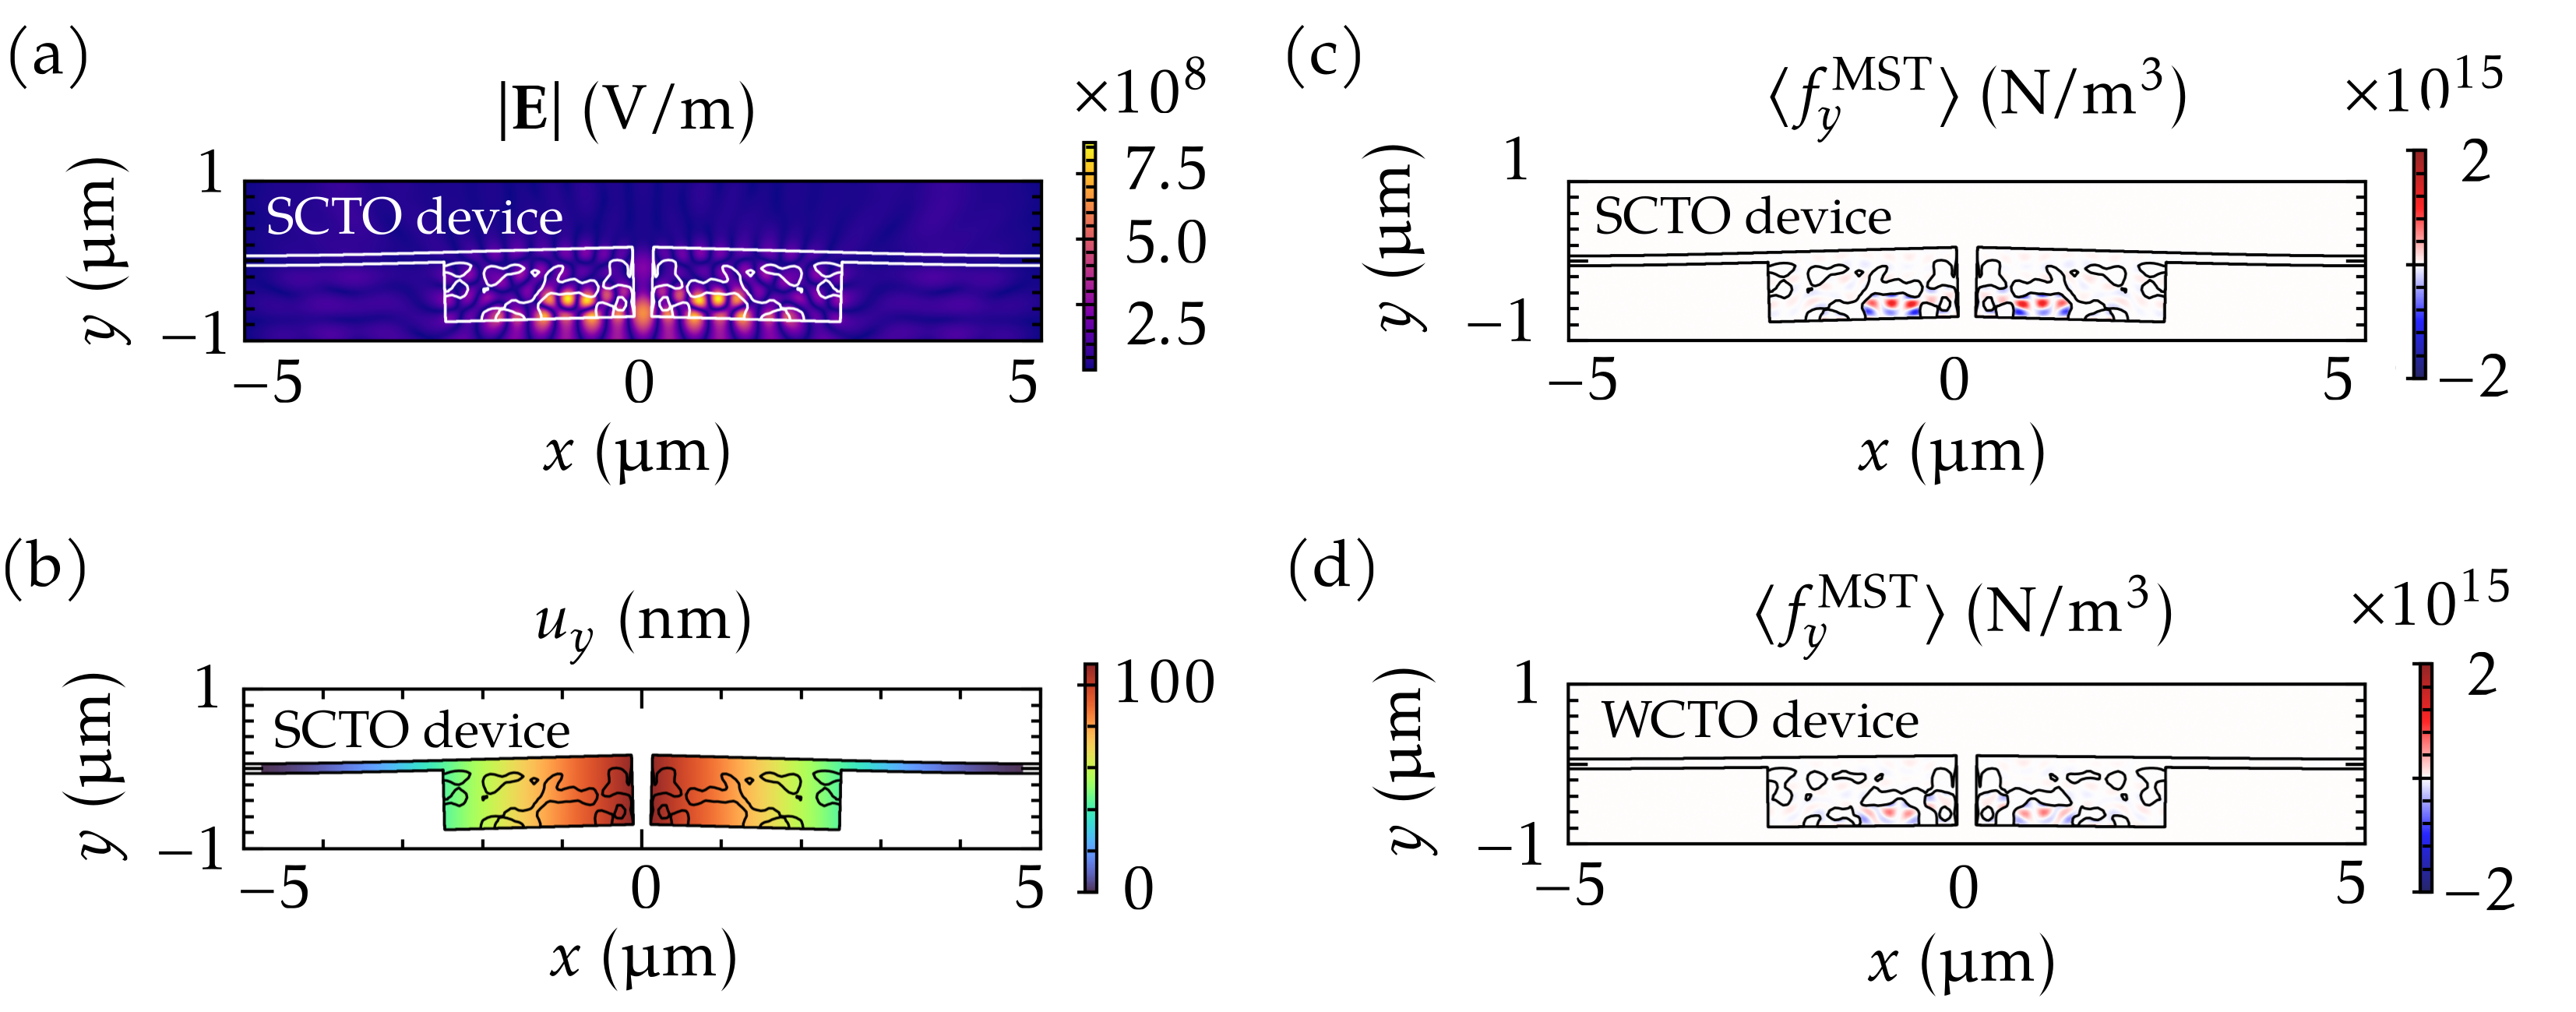
\includegraphics{figures/fields_panels_SC.png}}%%
    \caption{Device evaluation in the deformed material configuration. (a) Electric-field norm ($\vert\mathbf{E}\vert$) for the SCTO device.
     (b) Vertical ($y$) component of the MST force ($\langle f^\text{MST}_y\rangle$) for the SCTO device. (c) Vertical ($y$) component of
      the MST force ($\langle f^\text{MST}_y\rangle$) for the WCTO device. (d) Vertical displacement ($u_y$) for the SCTO device. Adapted from .}
    \label{fig:SC}
\end{figure}


Using this formalism, we optimize a membrane-like device with a central hole that spans its full height and separates it along the $x$-axis and find
    the results displayed in \figref{fig:SC}, for a device optimized accounting solving the strongy coupled problem ($\alpha = 1$, SCTO) and a device optimized solving the weakly coupled problem ($\alpha = 0$, WCTO).
    When evaluated with the fully coupled model, the SCTO device achieves a FOM of $\approx 110$\,nm, while the WCTO achieves only
     $\approx 43$\,nm, demonstrating a $\approx$3$\times$ improvement when the full coupling
      is included during optimization. Evaluating the WCTO under the
       weakly coupled model gives an FOM of $\approx$69\,nm, highlighting
        a significant performance drop due to neglecting coupling effects in the design process. 
        Based on the results in \figref{fig:SC}, we interpret that the improved performance of the SCTO stems from the fact that the sides of the device are disconnected,
         thus inducing rotation, and producing heterogeneous vertical displacements that strongly modulate 
         the optical force distribution. This results in optimized Bragg-mirror-like features that are slightly tilted compared to the WCTO design, thus being able to more effectively reflect the incoming field. For another
         optimization example refer to, where we also consider the optimization of connected optomechanical membrane-like devices.

\subsection*{Outlook and future work}

This topology optimization framework can be applied to a wide
 range of optomechanical devices and paves the way for future developments. 
 For example, extending the method to include clamping losses and three-dimensional designs
  would improve accuracy for high aspect-ratio membranes~\cite{aspect_ratio}, while including
   photoelastic effects would capture strain-induced refractive index changes~\cite{photoelasticity}.
    The framework also holds promise for cavity optomechanics~\cite{cav_opt} beyond the quasistatic
     regime by replacing the mechanical steady-state model with a frequency-domain solver. 
     Moreover, incorporating models like third-medium regularization~\cite{HuHu0} could enable the design of
      flexible or reconfigurable systems where large deformations and mechanical nonlinearities
       strongly affect optical performance.


\openright
\chapter{Electro-optical topology optimization problems}\label{chap:eo}
%\section{Electro-optical systems~\cite{ownpub4}}\label{sec:electro_optical}
Electro-optics describes the interaction between electricity and optics. Electricity involves the presence and flow of electric charges, which can generate electromagnetic fields (\eqref{eq:faraday}--\eqref{eq:Gauss_B}).
However, the main difference between electricity and optics is that the frequency of the electrical fields ($\omega_E$)
is much lower than for optical fields ($\omega_E \ll \omega $), so that they can generally be treated as static fields\footnote{Similarly, as discussed in \secref{sec:nanophotonics}, the size ($s$) of optical devices
is usually much smaller than the wavelength of the electrical fields ($s\ll \lambda_E $), and the field is effectively quasistatic.}.
The interaction between electricity and optics is used in a variety of technologies such as high-speed modulators for optical communications~\cite{modu, modu1, modu2, pockels}, switches~\cite{eo_switch}, electrically pumped lasers~\cite{laser,laser_pic}, and integrated photonic circuits~\cite{laser_pic}. 
These systems exploit mechanisms ranging from the electro-optic effect~\cite{eo_effect} to carrier-induced refractive index
 changes~\cite{c_i_n} to achieve efficient light manipulation and generation, bridging electro-optic principles with carrier-driven processes central to optoelectronics.

As a basic example of electro-optic coupling, one can consider the \textbf{electro-optic effect}\footnote{This is analogous to the thermo-optic effect presented in \secref{sec:to_effect}.}~\cite{eo_effect},
where the refractive index of a material ($n$) can be modified under the influence of an external (static) electric field. The linear term in the electro-optic effect is known as the
Pockels effect $
    \Delta n = -(1/2) n^3 r E\,,$
where $r$ is the electro-optic coefficient, and $E$ is the applied electric field~\cite{pockels}. The quadratic term 
is the electro-optic Kerr effect $\Delta n = n_2 E^2$, where $n_2$ is the Kerr-coefficient~\cite{phot_crys}. Note that based on the applied external
quasistatic electric field, one can model the refractive index change by accounting for higher order terms in the expansion of the polarizability
in terms of the electric field (\eqref{eq:polarization}), where the Pockels effect corrresponds to the $\chi^{(2)}$ term, and the Kerr effect to the $\chi^{(3)}$ term.

Building on this understanding of electro-optic phenomena, topology optimization has been extensively applied to design coupled electrical systems such as electromechanical~\cite{MEMS_multi,electrostatic_act} or electrochemical~\cite{electrode} systems. However, electro-optics remains relatively unexplored, with only a few studies, such as~\cite{g_heat}, which focuses on diffusion-based designs for carrier dynamics in semiconductor devices.

In the remainder of the section, we focus on our work~\cite{ownpub4}, in which we apply topology 
optimization to design a nanolaser device, where electrical pumping can be used to achieve efficient light emission.

\section{Topology optimization of nanolasers~\cite{ownpub4}}\label{sec:laser}

\subsection*{A figure of merit for nanolaser performance}

A nanolaser is a nanoscale device that emits light by stimulating the emission of photons in a gain medium, which is typically a semiconductor material. This is illustrated
in \figref{fig:laser2d}, where a pump laser excites the emitters or carriers (e.g., electrons and holes) in a gain medium $D_0$, which then emits light into an output channel (e.g., waveguide) via
stimulated emission. This physical
mechanism can be described by using the Maxwell-Bloch equations~\cite{haken_laser_dynamics, PhysRev.134.A1429, SALT_original}, which are a set of nonlinear time-dependent 
partial differential equations. When aligned to high-quality-factor ($Q \sim$ lifetime/period)~\cite{phot_crys} lasing mode ($Q\gtrapprox 100$~\cite{cerjan_2016}), the Maxwell-Bloch equations can be simplified via the single-pole approximation (SPA-) steady-state ab-initio laser theory (SALT)~\cite{Ge_2010}, leading to
\begin{equation}\label{eq:SPA_SALT}
    \left[(\nabla \times 
     \nabla \times ) -\left[\varepsilon_c(\mathbf{r})-i \Delta \varepsilon^{\prime \prime} (\mathbf{r})\right] \left(\frac{\omega_L}{c}\right)^2\right] \mathbf{E}_L(\mathbf{r})=0\,,
\end{equation}
where $\mathbf{E}_L$ is the lasing mode, $\omega_L$ is the lasing frequency, $\varepsilon_c$ is the dielectric permittivity of the passive (no gain) cavity, and the change in the 
imaginary part of the permittivity is given by
\begin{equation}\label{eq:gain_SALT}
        \Delta \varepsilon^{\prime \prime} (\mathbf{r}) =  \frac{D_0(\mathbf{r}) d_\text{pump}}{1+ e_c^{-2}\left|\mathbf{E}_L(\mathbf{r})\right|^2}\,,
\end{equation}
where $D_0$ is the gain profile, $d_\text{pump}$ is a scalar pumping strength, and $e_c$ is a non-dimensionalization parameter~\cite{Ge_2010}. While the SPA-SALT model (\eqref{eq:SPA_SALT}) 
is simpler and can be solved more efficiently than the Maxwell-Bloch equations, it still requires one to solve a nonlinear eigenproblem. This can be computationally expensive, especially in 
inverse design tasks where hundreds or thousands of such problems must be solved to optimize a device.

\begin{figure}[tb]
    \centering
    \makebox[\textwidth][c]{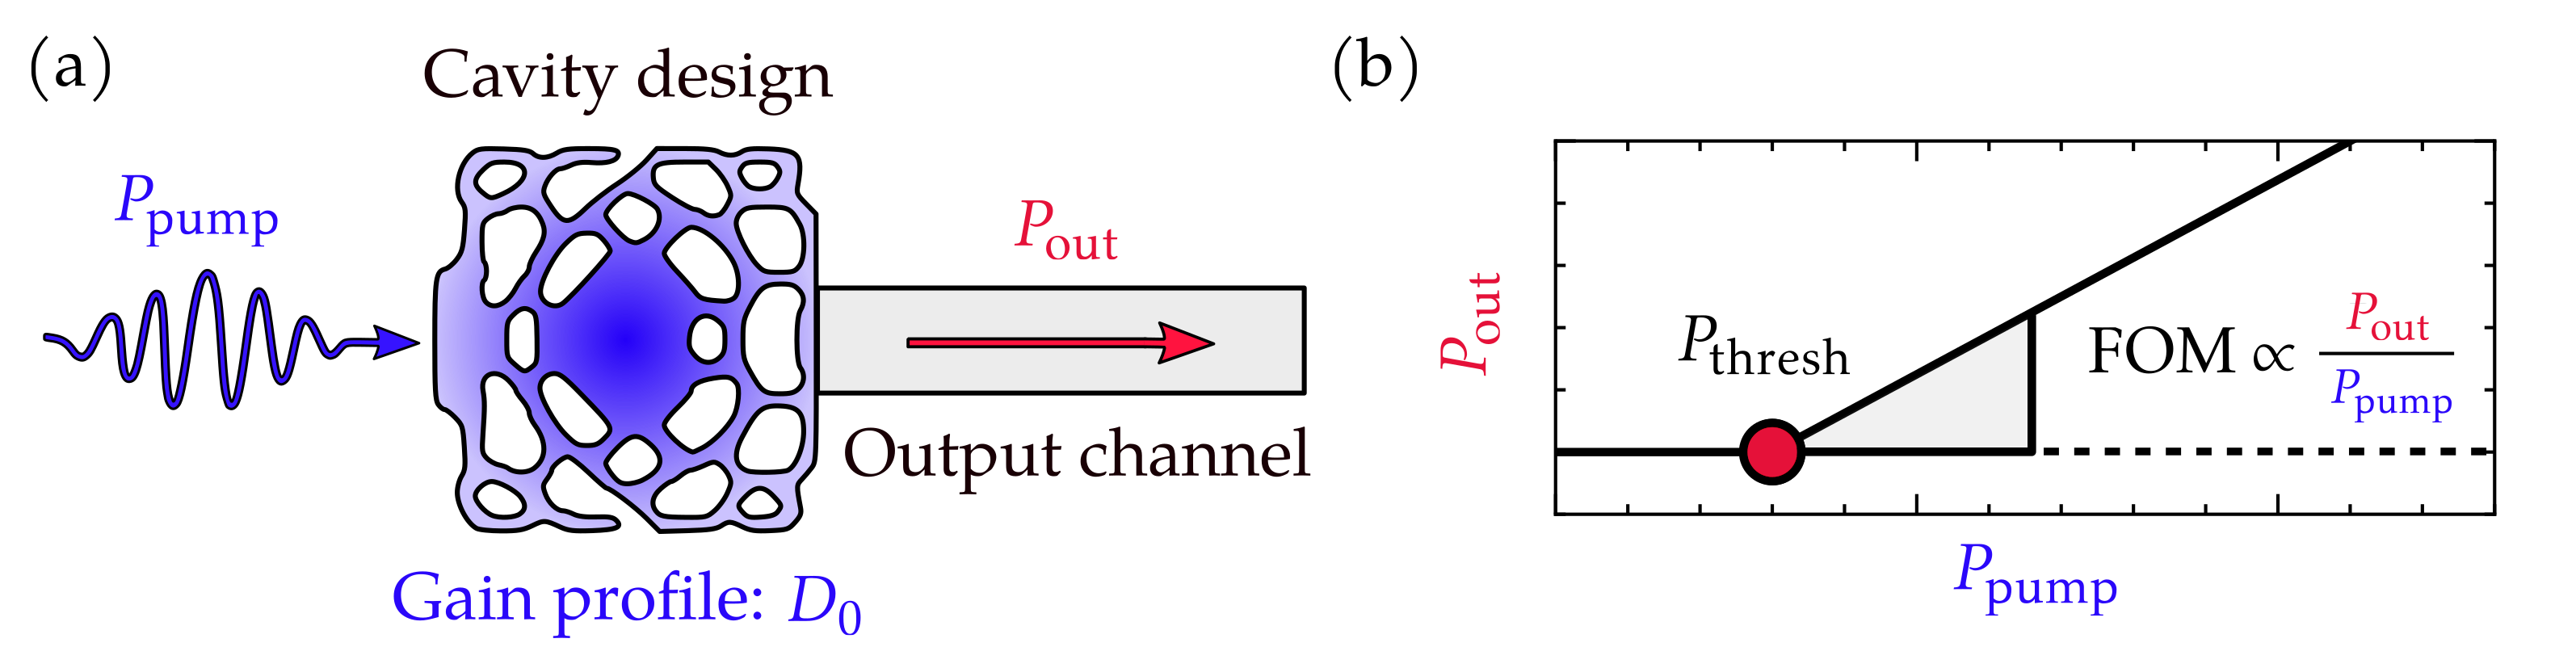
\includegraphics{figures/laser.png}}%%
    \caption{Topology optimization of nanolasers. (a) Working principle of a nanolaser. A pump with power $P_\text{pump}$ excites a gain medium with profile
    $D_0$ that emits a single lasing mode into an output channel with power $P_\text{out}$. (b) The optimization FOM is proportional to the linear relation between the pump and output power ($P_\text{out}/P_\text{pump}$),
    just above the lasing threshold ($P \gtrapprox P_\text{thres}$).  Figure adapted from~\cite{ownpub4}.}
    \label{fig:laser2d}
\end{figure}

To circumvent this, in~\cite{ownpub4}, we propose a synthesis of SPA-SALT, perturbation theory, and coupled mode theory to simplify the problem. 
The two key results of this derivation are the expression of the lasing threshold and the FOM for nanolaser design, which can be evaluated by solving a linear system of equations.
The expression for the \textbf{lasing threshold} is given by~\cite{ownpub4}
\begin{equation}\label{eq:pump_thresh}
 d_\text{thresh} = \frac{1}{\Gamma Q} = \frac{1}{Q} \frac{\int_{\Omega} \varepsilon_c(\mathbf{r})|\mathbf{E}_{\text{r}}(\mathbf{r})|^2\, \d \Omega}{\int_{\Omega} D_0(\mathbf{r}) |\mathbf{E}_{\text{r}}(\mathbf{r})|^2\, \d \Omega}\,,
\end{equation}
where $\mathbf{E}_\text{r}$ is the field in a reciprocal problem (\eqref{eq:reciprocity}), in which the system is excited from an output port\footnote{In a high-$Q$ system, the field from the reciprocal solve $\mathbf{E}_r$ is almost exactly equal to the cavity mode and/or the lasing mode plus a $\mathcal{O}(1/\sqrt{Q})$ error~\cite{phot_crys}.} (e.g. the waveguide in \figref{fig:laser2d}), and $\Gamma$ is a measure 
of energy confinement in the gain region. From this expression, one can reduce the lasing threshold by increasing $Q$ and enhancing the energy confinement in the
active medium ($\Gamma$). In the single-emitter limit, where an emitter located at position \(\mathbf{r}^\prime\) is modeled as 
\(D_0(\mathbf{r}) \propto \delta(\mathbf{r} - \mathbf{r}^\prime)\), 
the expression for the lasing threshold reduces  reduces to \(d_{\text{thresh}} = V / Q\), where $V$ is a measure of the modal volume. This is a common FOM in inverse design problems outside of lasers (e.g.,~\cite{LDOS_opt_wang}) and is closely
related to the local density of states ($ \text{LDOS} \propto Q/V$)~\cite{LDOS_opt_wang}.
   Note that evaluating this lasing threshold expression (\eqref{eq:pump_thresh}) still requires solving an eigenproblem to determine \(Q\).


The second key result of the work is \textbf{a FOM for nanolaser design} that is proportional to the laser efficiency ($\propto P_\text{out}/P_\text{pump}$) and that in contrast to the lasing threshold (\eqref{eq:pump_thresh}) can be evaluated without solving an eigenproblem, through a single reciprocal solve~\cite{ownpub4}
\begin{equation}\label{eq:eff_nl}
    \frac{P_\text{out}}{P_\text{pump}} \propto \frac{\left( \int_{\Omega} D_0(\mathbf{r})|\mathbf{E}_{\text{r}}(\mathbf{r})|^2 \,  \d \Omega \right)^3} {\int_{\Omega} D_0(\mathbf{r}) |\mathbf{E}_{\text{r}}(\mathbf{r})|^4 \,  \d \Omega} = \text{FOM}.
\end{equation}
We refer to this FOM as the \emph{nonlinear} FOM, since it accounts for the laser nonlinearities perturbatively. The FOM is roughly proportional 
to the energy in the cavity ($\sim |\mathbf{E}_{\text{r}}|^6 / |\mathbf{E}_{\text{r}}|^4 \sim |\mathbf{E}_{\text{r}}|^2$), and thus to the $Q$ factor\footnote{This also contributes to attaining a low
laser threshold (\eqref{eq:pump_thresh}).}. Consequently, as the optimization progresses, the high-$Q$ assumption in SPA-SALT (\eqref{eq:SPA_SALT}) will become increasingly accurate. In the single emitter limit, the FOM becomes
$\text{FOM}=\vert \mathbf{E}_{r}(\mathbf{r}^\prime) \vert^2$, which resembles an LDOS-like quantity in the reciprocal problem formulation~\cite{reci} and is proportional to the total power emitted into an output channel~\cite[App.~C]{reci}. 

To show how the nonlinear FOM compares to more conventional cavity-optimization approaches, we introduce a “naive” generalization of the LDOS, which heuristically modifies the definition
of the LDOS to account for out-coupling efficiency [through a reciprocal solve ($\mathbf{E}_r$)] and a distributed gain
medium
\begin{equation}\label{eq:SEL}
 \text{FOM}_{\text {naive }}=\int_{\Omega} D_0(\mathbf{r})\left|\mathbf{E}_{\text{r}}(\mathbf{r})\right|^2 \d \Omega\,,
\end{equation}
which we refer to as the \emph{naive} FOM, defined by the overlap of the electric-field intensity of the reciprocal field with the gain distribution.
This naive FOM is also proportional to the intensity of the reciprocal field ($\sim |\mathbf{E}_{\text{r}}|^2$), and thus roughly proportional to $Q$, and should also result in 
high-$Q$ optimized cavities. Note that this FOM also describes the case of a single-point gain region (e.g., a quantum dot),
whose location is randomly distributed in the cavity with a probability density $\mathcal{P} \sim D_0$. 

\subsection*{Optimization results for extended gain media}

\begin{figure}[tb]
    \centering
    \makebox[\textwidth][c]{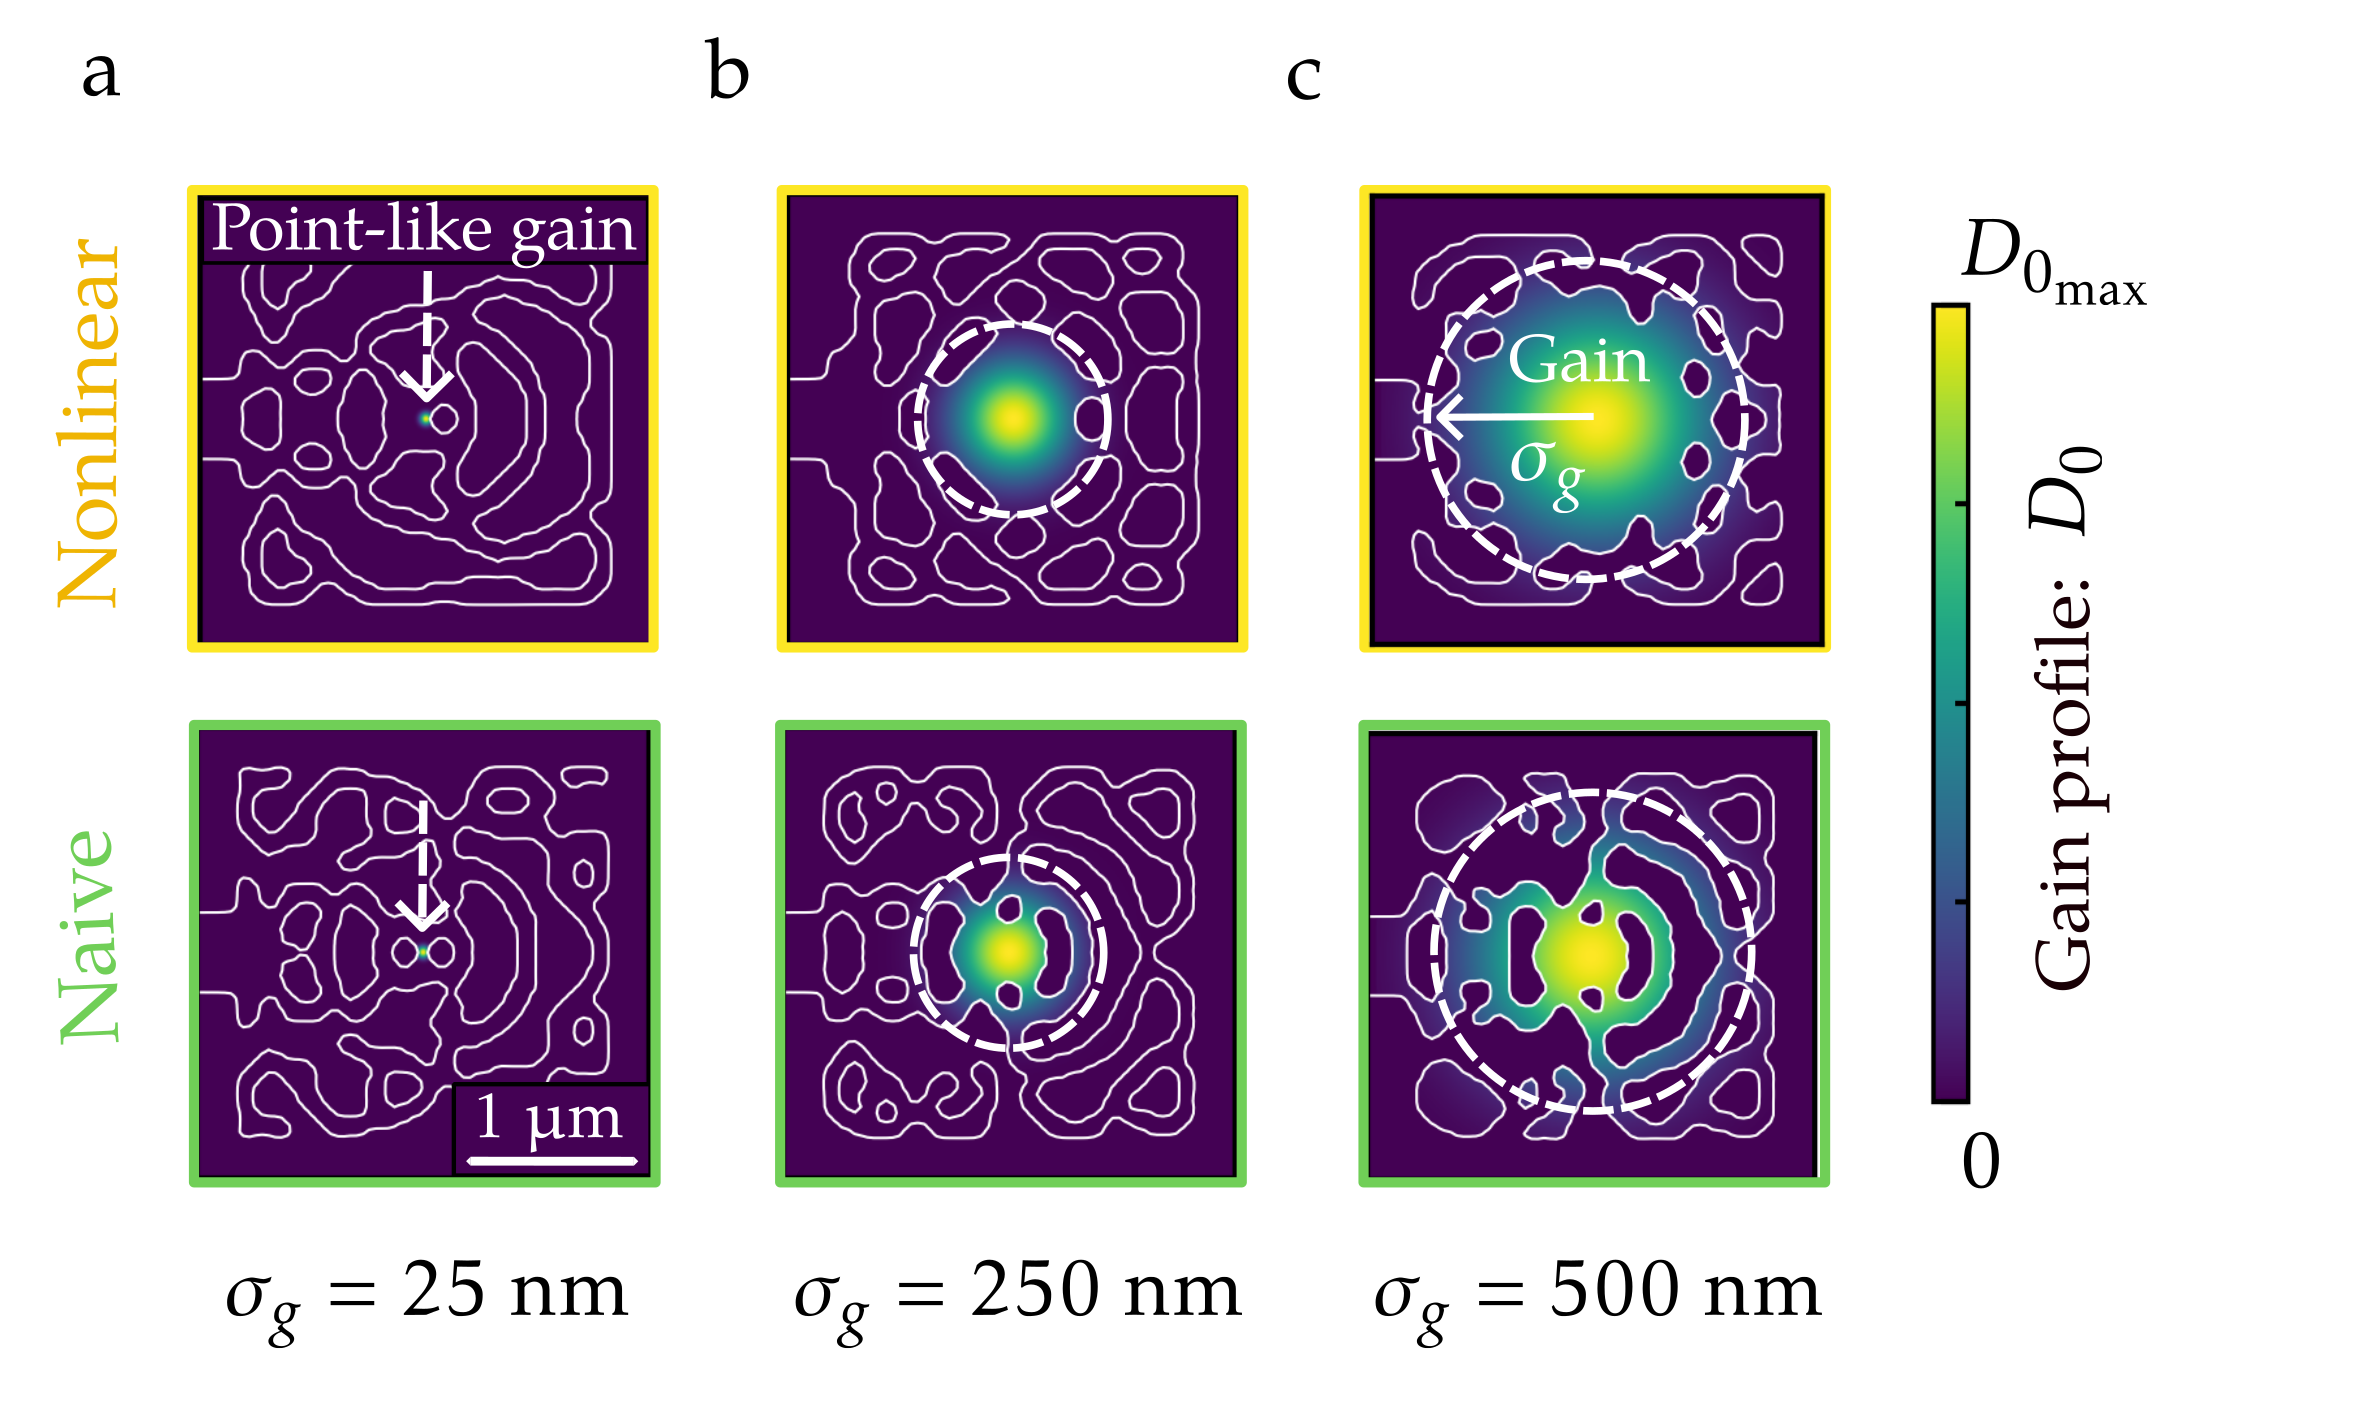
\includegraphics{figures/laser_size.png}}%%
    \caption{Topology-optimized devices when targeting the nonlinear and naive FOMs for different Gaussian gain distributions with standard deviations $\sigma_g$. (a) Device optimize for a point-like gain region ($\sigma_g=25$ nm).
    (b) Device optimized for $\sigma_g=250$ nm. (c) Device optimized for $\sigma_g=500$ nm. Figure adapted from~\cite{ownpub4}.}
    \label{fig:laser_size}
\end{figure}

Using the formalism introduced in the last subsection, we optimize two-dimensional nanolasers and study the influence of the gain region size in 
nanolaser design (\figref{fig:laser_size}). A design-dependent Gaussian distribution centered around the center, $\mathbf{r}_0$, of the cavity, describes the gain medium as
\begin{equation}
D_0 (\mathbf{r}, \hat{\rho}) = \varepsilon_{\text{r}}(\mathbf{r})  \hat{\rho}(\mathbf{r}) \, e^{- \vert \mathbf{r}- \mathbf{r}_0 \vert^2 / 2 \sigma_{\text{g}}^2 }\,,
\end{equation}
where
$\sigma_g$ is the standard deviation of the Gaussian and acts as a measure of the gain region size. We verify that for point-like gain regions, the devices optimized for the FOM and the naive FOM (\eqref{eq:SEL})
achieve similar performance (limited by the finite size of the tiny gain region), favoring bowtie-like cavity designs
where the in-plane electric field is concentrated at a bowtie sharpness-limited field singularity~\cite{sing}. Moreover, we show that for distributed gain media with sizes comparable to the wavelength 
($\sigma_g \sim \lambda$, for $\lambda = 1.55$~\textmu m), 
the derived FOM, in contrast to the naive FOM, discourages field localization due to the quartic field term in the denominator of~\eqref{eq:eff_nl} 
(since $\int |\mathbf{E}|^2$ is finite). 
This results in an approximate $3\times$ enhancement when targeting the correct (nonlinear) nanolaser FOM~\eqref{eq:eff_nl}.

\subsection*{Accounting for gain diffusion}

In semiconductors with extended gain media, it is essential to model the electrical effect of \textbf{carrier diffusion}. This effect can be introduced by modeling the semiconductor gain medium in the free-carrier approximation\footnote{Neglecting carrier-carrier Coulomb interactions.}, using a diffusion 
equation~\cite{csalt}. Using this formalism, we re-derive the expression for the lasing threshold (\eqref{eq:pump_thresh}) when accounting for carrier diffusion effects~\cite{ownpub4}, which gives
\begin{equation}\label{eq:pump_thresh_diff}
 d_\text{thresh} = \frac{1}{Q} \frac{\int_{\Omega} \varepsilon_c(\mathbf{r})|\mathbf{E}_{\text{m}}(\mathbf{r})|^2\, \d \Omega}{\int_{\Omega} \mathbb{S} [D_0] (\mathbf{r}) |\mathbf{E}_{\text{m}}(\mathbf{r})|^2\, \d \Omega}\,,
\end{equation}
and the nanolaser FOM (\eqref{eq:eff_nl}) with carrier diffusion effects, which yields
\begin{equation}\label{eq:eff_diff}
 \text{FOM} =  \frac{\left(\int_{\Omega} \mathbb{S} [D_0](\mathbf{r}) |\mathbf{E}_{\text{r}}(\mathbf{r})|^2 \, \d \Omega\right)^3} {\int_{\Omega} \mathbb{S}\left[ |\mathbf{E}_{\text{r}}|^2\, \mathbb{S} [D_0] \right] (\mathbf{r})|\mathbf{E}_{\text{r}}(\mathbf{r})|^2 \, \d \Omega}\,.
\end{equation}
These expressions use the diffusion operator $\mathbb{S}^{-1}= \mathbb{I}+\nabla \cdot (R_\nabla^2 \nabla)$, where $\mathbb{I}$ is the identity operator, and $R_\nabla (\mathbf{r})$ is a design-dependent diffusion lengthscale.
In this notation, computing $u = \mathbb{S}[b]$ corresponds to solving for the scalar field $u$ in the diffusion problem $\mathbb{S}^{-1}u=b$, where $b$ is a scalar field. 
The main difference when accounting for diffusion is that now one needs to consider the profile of diffused carriers ($\mathbb{S} [D_0]$) in the lasing threshold (\eqref{eq:pump_thresh_diff}), and the diffusion of the gain depletion ($\mathbb{S}[ |\mathbf{E}_{\text{r}}|^2\, \mathbb{S} [D_0]]$)
in the FOM denominator (\eqref{eq:eff_diff}). Note that in the small diffusion limit ($R_\nabla \ll \lambda, \mathbb{S} \approx \mathbb{I}$)
we recover the original expressions in \eqref{eq:pump_thresh} and \eqref{eq:eff_nl}.

\begin{figure}[tb]
    \centering
    \makebox[\textwidth][c]{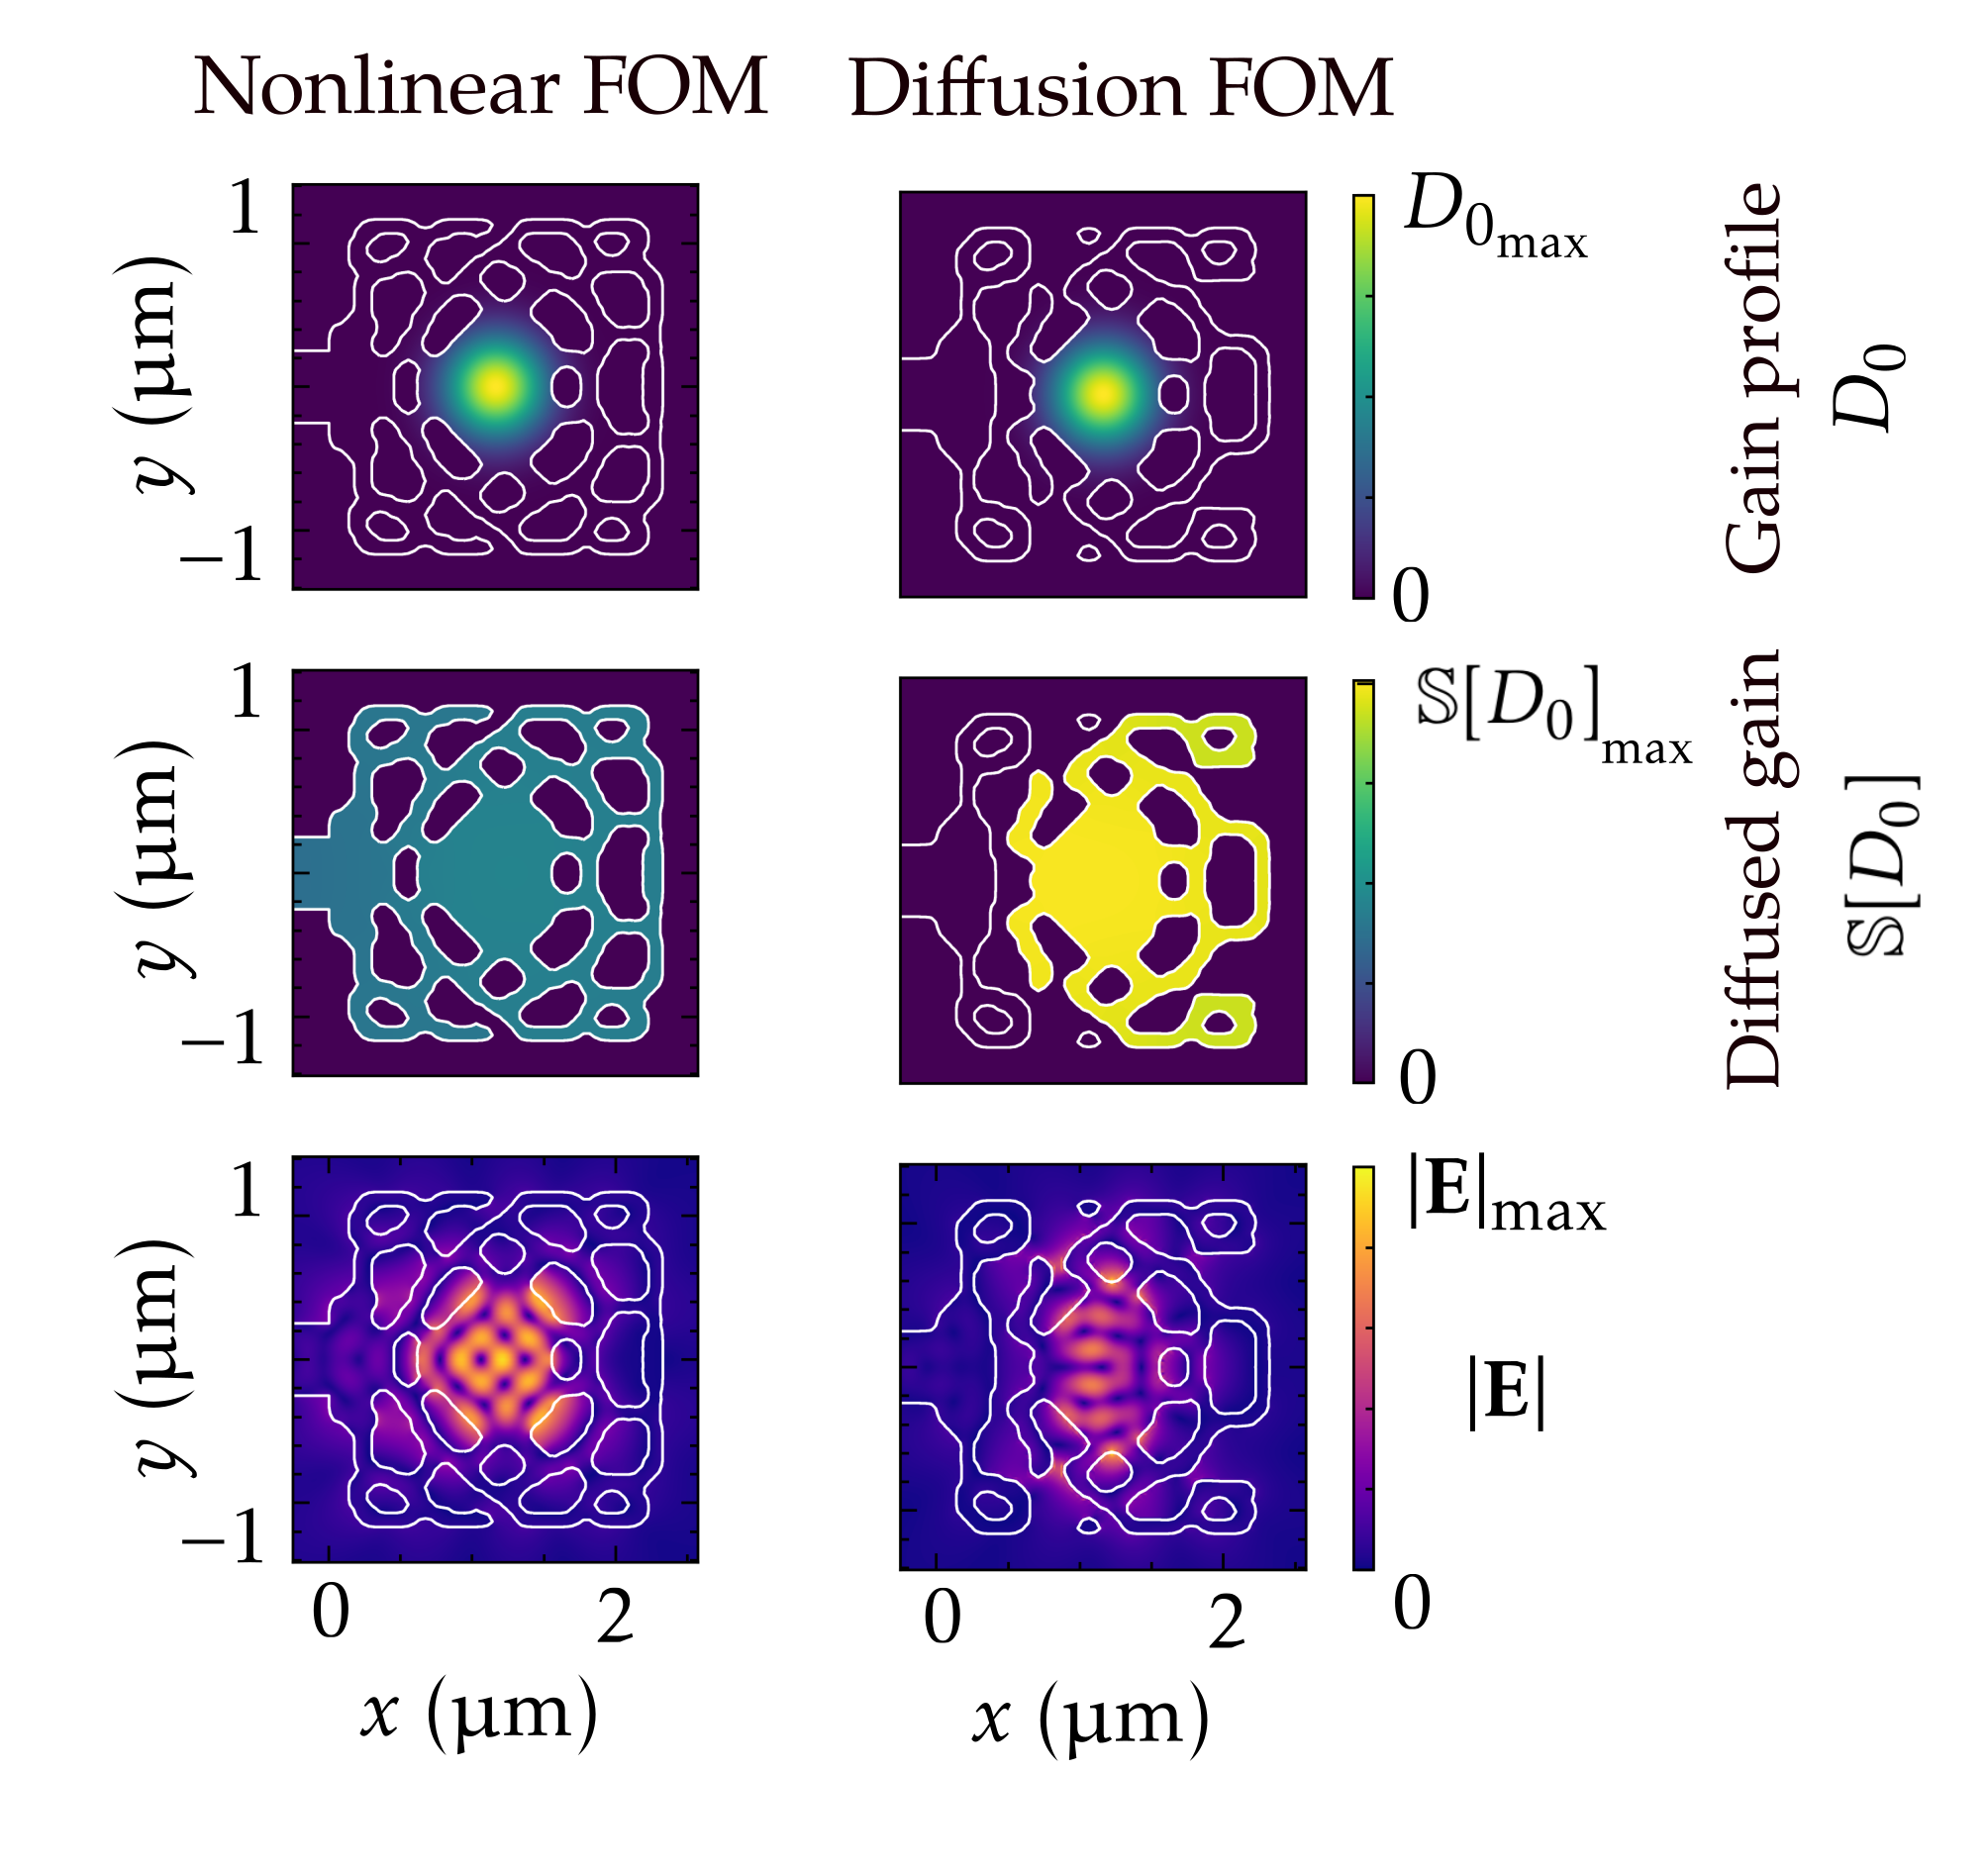
\includegraphics{figures/laser_carriers.png}}%%
    \caption{Topology-optimized devices with gain diffusion effects for a gain region with size $\sigma_g=250$ nm and a diffusion length of $R_\nabla=5$ \textmu m. The device optimized without accounting for gain diffusion ("Nonlinear FOM") and the device optimized accounting for gain diffusion ("Diffusion FOM") have the gain profile $D_0$ that is diffused ($\mathbb{S}[D_0]$)
    in the semiconductor-like material, and generate the optical field given by the electric-field norm $\vert \mathbf{E} \vert$. Figure adapted from~\cite{ownpub4}.}
    \label{fig:laser_diff}
\end{figure}

By using the expression in \eqref{eq:eff_diff} as an optimization FOM, we study how accounting for diffusion
affects the design and performance of nanolasers. As shown in \figref{fig:laser_diff}, the device that accounts for diffusion disconnects the cavity from the waveguide while also removing
material from areas of weak electric field to 
enhance the coupling between the carriers and the optical field, and results in a $\approx 2\times$ enhancement when considering the diffusion-corrected FOM. 

\subsection*{Towards realizable nanolasers: three-dimensional designs}

Finally, we apply the formalism to design three-dimensional silicon-on-insulator nanolasers (\figref{fig:laser3d}). 
We verify that, similar to the two-dimensional case, the FOM discourages field localization while still efficiently coupling to the output waveguide, yielding a $\approx 1.6\times$
enhancement when considering the correct nonlinear FOM for extended gain media (\eqref{eq:eff_nl}). We attribute the enhancement drop with respect to the two-dimensional optimization results to the fact that localizing a high-$Q$ resonance is more difficult in three dimensions, due to out-of-plane radiation losses.

\begin{figure}[tb]
    \centering
    \makebox[\textwidth][c]{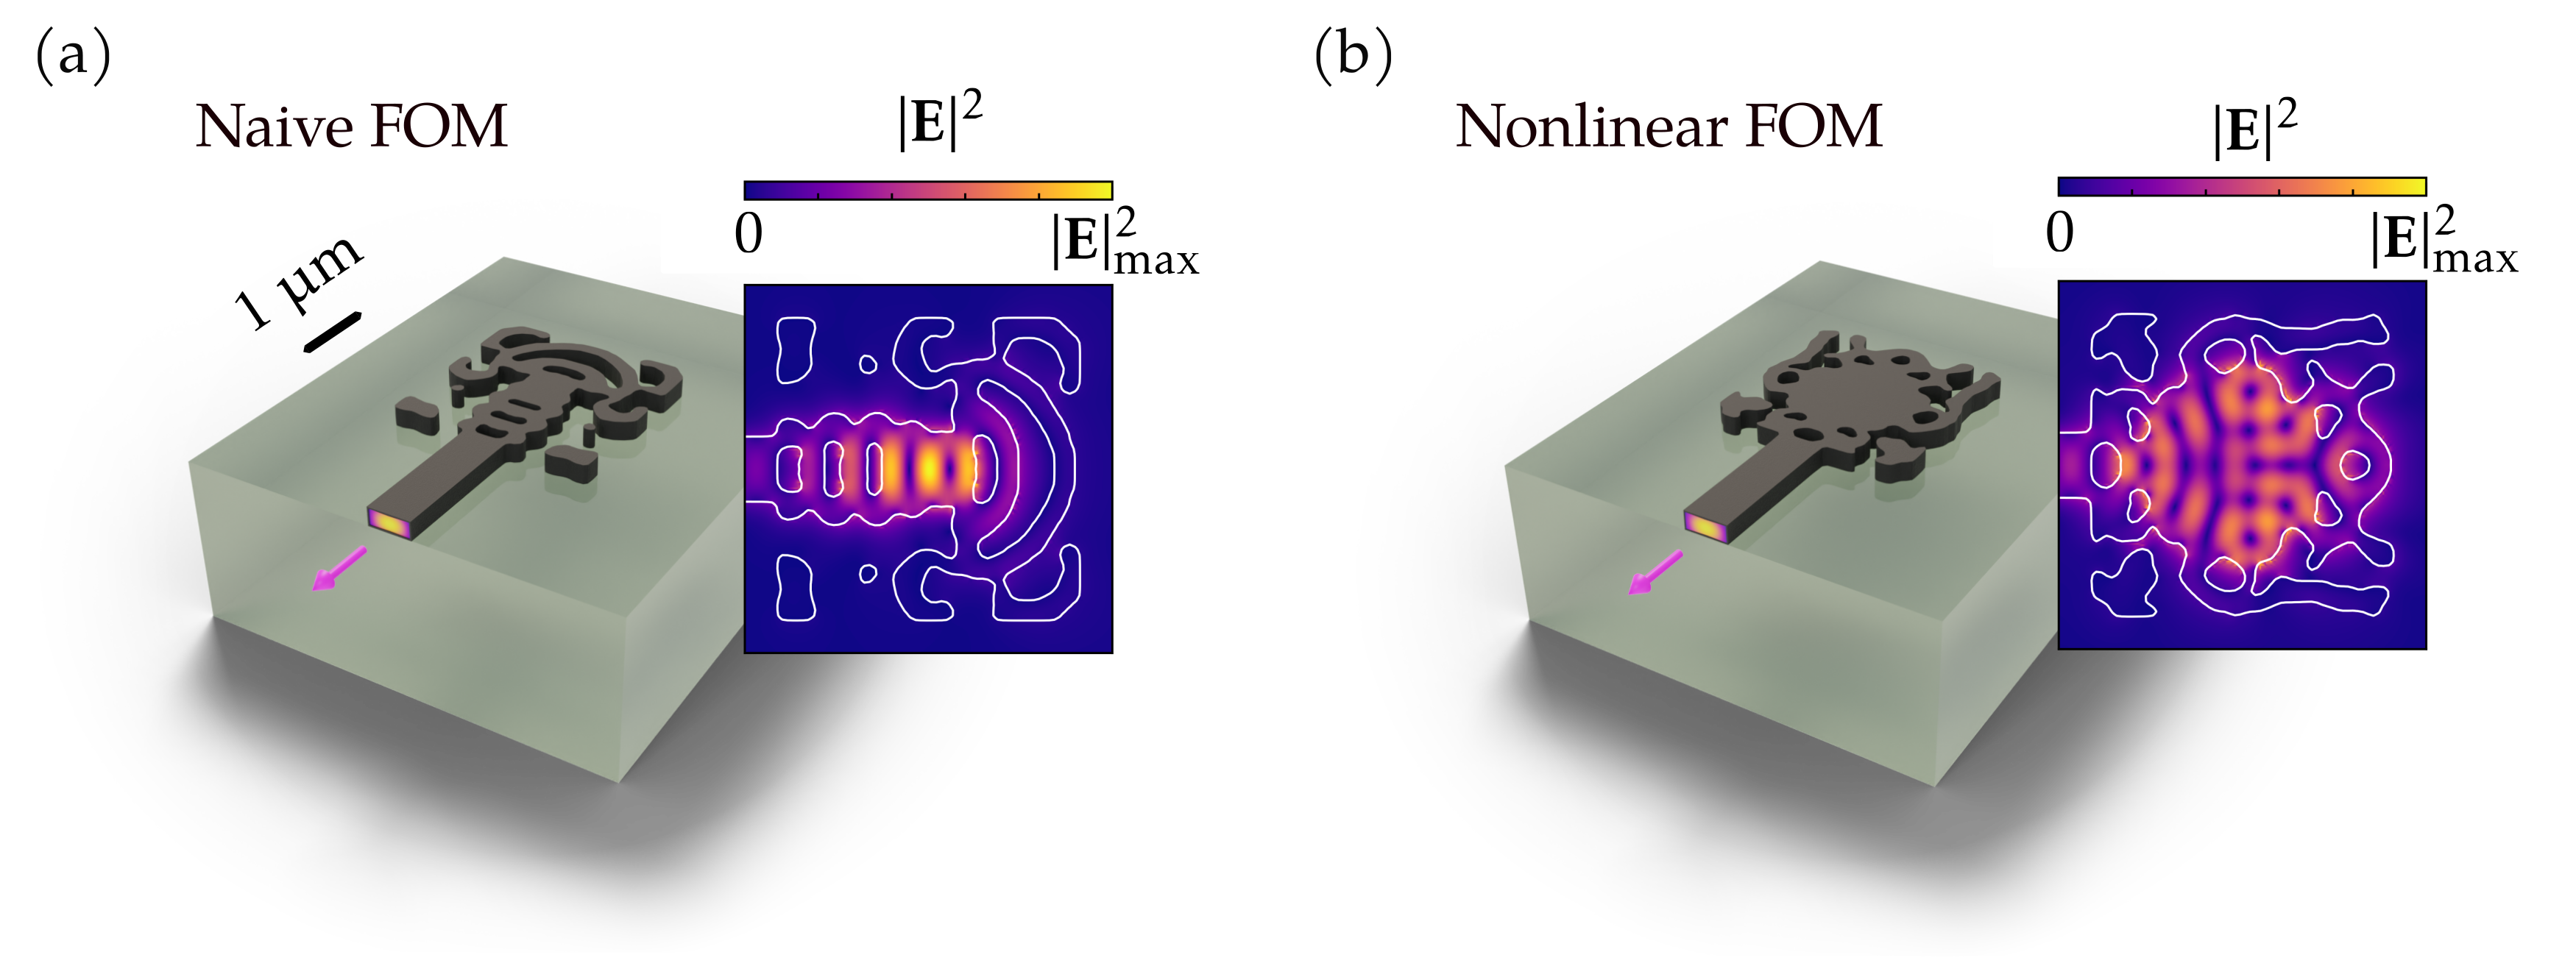
\includegraphics{figures/laser_2.png}}%%
    \caption{Topology-optimized nanolasers in three dimensions. The devices lase into the cavity mode (inset plot) and out-couple to the waveguide mode. (a) Device optimized for the naive FOM. (b) Device optimized for the nonlinear FOM.
    Figure adapted from~\cite{ownpub4}.}
    \label{fig:laser3d}
\end{figure}

\subsection*{Outlook and future work}

In conclusion, in \cite{ownpub4} we show that by exploiting perturbative analysis valid in high-$Q$ cavities, one can derive  
an efficient FOM for laser performance ($\propto P_\text{out}/P_\text{pump}$) that captures resonant enhancement,  
spatial hole-burning, and gain diffusion at little extra computational cost. The FOM evaluation requires only a  
single linear reciprocal Maxwell solve (plus potentially two scalar solves for gain diffusion), making it 
an efficient formulation for laser optimization. This efficient first-principles approach allows for inverse nanolaser design in two and three dimensions, while  
also allowing for future refinements, including accounting for the laser linewidth~\cite{pick}, or accurate pumping models, where optical or electrical pumping could be explicitly
modeled by solving an additional partial differential equation.

\openright
\chapter{Concluding remarks}

This thesis presents a comprehensive study on multiphysics topology optimization in nanophotonics, focusing on the development of novel design methods for applications that rely on coupled physical effects, such as thermo-optical, optomechanical, and electro-optical interactions.

It begins by introducing the field of nanophotonics (\secref{sec:nanophotonics}) and the numerical solution of Maxwell's equations (\secref{sec:fem}), which form the foundation for topology optimization in the single physics picture. The framework is then extended to multiphysics problems (\secref{sec:coupled}), including a general multiphysics topology optimization formulation (\secref{sec:topopt_theory}).

Thermo-optical topology optimization is addressed next (\chapref{chap:eo}), where heat transfer is coupled to Maxwell's equations. Several coupling mechanisms are considered, with a focus on designing low-loss thermo-optical phase shifters (\secref{sec:TOPS}) by strategically placing metallic heaters around optical waveguides.

The thesis then explores optomechanical topology optimization (\chapref{chap:om}), including the design of particles and their environments for optical force manipulation (\secref{sec:engi}), photonic cavities for sub-wavelength particle trapping (\secref{sec:dip}), and membrane structures whose optical response is modulated by mechanical deformation (\secref{sec:mech_strongly_coupled}).

Finally, electro-optical topology optimization is investigated (\chapref{chap:eo}), with an efficient design formulation for nanolaser devices (\secref{sec:laser}). Here, the interplay between carrier dynamics and optical modes is shown to be critical for optimizing device performance. 

Overall, this research contributes to the design of novel nanophotonic devices that leverage multiphysics interactions, enabling enhanced functionality, improved performance, and new capabilities in nanophotonic systems.
\section{Future work}

This work opens several avenues for future research, including:

\begin{itemize}
    \item \textbf{Application to experimental setups:} While the framework was developed theoretically, it can be adapted to specific experimental configurations with minor, problem-dependent modifications.
    
    \item \textbf{Nonlinear multiphysics extensions:} The current adjoint formulation (\secref{sec:topopt_theory}) handles cascaded nonlinear dependencies in coupled systems, where the couplings are nonlinear but physics system can still be solved linearly. Future work could consider Future work could extend this to fully nonlinear systems, where each governing equations depend on their respective state solution.
    
    \item \textbf{Simultaneous multiphysics effects:} Extending the framework to handle multiple coupled effects, such as thermo-electro-optical interactions or combined geometric deformation and photoelasticity (\secref{sec:mech_strongly_coupled}), could unlock advanced device functionalities.
    
    \item \textbf{Advanced figures of merit (FOMs):} In some works more complex FOMs could be explored. As an example, in the optical force engineering problem (\secref{sec:engi}), one could target optical torque (\eqref{eq:torque}) or design the spatial distribution of forces for engineered particle motion.
    
    \item \textbf{Strongly coupled systems:} Beyond the optomechanical membrane case, other strongly coupled problems, like heat-induced refractive index changes from optical absorption (\secref{sec:thermo_strong_coupling}), could be investigated.
    
    \item \textbf{Nanolaser pumping models:} The nanolaser topology optimization framework (\secref{sec:laser}) could be extended to include explicit models of optical or electrical pumping.
\end{itemize}

\newrefcontext[labelprefix=]
\printbibliography[notkeyword=myPub,notkeyword=myMan]


\appendix
\chapter{Appendix}
\section{Sensitivity analysis for weakly coupled multiphysics problems}\label{app:appendix1}
In this appendix, we derive the adjoint sensitivity expressions for a general weakly coupled multiphysics
 problem with $N$ physics. The system is written as $\mathbf{K}\mathbf{u} = \mathbf{f}$, where $\mathbf{K}$ is 
 the stiffness matrix of the coupled system, $\mathbf{u}$ is the solution vector, and $\mathbf{f}$ is the source or forcing term vector. For 
 simplicity, we assume real-valued problems, but this method can be extended to complex-valued cases, as shown
  in~\cite{ownpub0} for a simple two-physics ($N=2$) example. As described in~\secref{sec:coupled}, 
  for $N$ physics with \textbf{weak nonlinear coupling} (\eqref{eq:multiphysics_weak_nonlinear}), the full 
  system is upper or lower triangular, as in
\begin{equation} \label{eq:app_multiphysics_weak}
    \begin{bmatrix}
        \mathbf{K}_1(\mathbf{u}_2, \cdots \mathbf{u}_N)    & \mathbf{C}_{12} (\mathbf{u}_2, \cdots \mathbf{u}_N)& \cdots & \mathbf{C}_{1N}(\mathbf{u}_2, \cdots \mathbf{u}_N) \\
        0 & \mathbf{K}_2 (\mathbf{u}_3, \cdots \mathbf{u}_N)   & \cdots & \mathbf{C}_{2N} (\mathbf{u}_3, \cdots \mathbf{u}_N)\\
        \vdots          & \vdots          & \ddots & \vdots          \\
        0& 0 & \cdots & \mathbf{K}_N
    \end{bmatrix}
    \begin{bmatrix}
        \mathbf{u}_1 \\
        \mathbf{u}_2 \\
        \vdots       \\
        \mathbf{u}_N
    \end{bmatrix}
    =
    \begin{bmatrix}
        \mathbf{f}_1\\
        \mathbf{f}_2\\
        \vdots       \\
        \mathbf{f}_N
    \end{bmatrix}\,,
\end{equation}
where we have chosen the upper diagonal version of the weakly coupled problem and the system of equations has been rewriten in terms of the stiffness ($\mathbf{K}_i$) and 
coupling matrices ($\mathbf{C}_{ij}$) so that the right-hand-side $\mathbf{f}=[\mathbf{f}_1, \cdots, \mathbf{f}_N]^\top$ does not depend
on the solution vector $\mathbf{u}=[\mathbf{u}_1, \cdots, \mathbf{u}_N]^\top$. This notation is equivalent to having $N$ equations of the form
\begin{align}
\left\{
    \begin{aligned}
        \quad \mathbf{K}_1(\mathbf{u}_2, \ldots, \mathbf{u}_N)\, \mathbf{u}_1  + \sum_{j=2}^N \mathbf{C}_{1j} (\mathbf{u}_2, \cdots \mathbf{u}_N)\, \mathbf{u}_j &= \mathbf{f}_1\,, \\
        \quad\mathbf{K}_2(\mathbf{u}_3, \ldots, \mathbf{u}_N)\, \mathbf{u}_2 + \sum_{j=3}^N \mathbf{C}_{2j} (\mathbf{u}_3, \cdots \mathbf{u}_N)\, \mathbf{u}_j &= \mathbf{f}_2\,, \\
        \quad\ldots \\
        \quad\mathbf{K}_{N-1} (\mathbf{u}_N) \, \mathbf{u}_{N-1} + \mathbf{C}_{N-1\, N}(\mathbf{u}_N)\, \mathbf{u}_N &= \mathbf{f}_{N-1} \,, \\
        \quad\mathbf{K}_N \, \mathbf{u}_N &= \mathbf{f}_N\,.
    \end{aligned}
\right.
\end{align}
In this case, we can solve the system of equations sequentially in a \textbf{seggregated} fashion,
 where problem $i=N$ is solved first, and the solution is used to solve the next problem ($i=N-1$), and so on, until the first problem ($i=1$) is solved
 (as in the sequence: $\mathbf{u}_N \to \mathbf{u}_{N-1} \to \cdots \to \mathbf{u}_1$).\\

To calculate the sensitivites using the adjoint method we start by rewriting the FOM ($\Psi$) by adding the residual
of the state equations, multiplied by a set of Lagrange multipliers ($\Lambda_i$)
\begin{equation}\label{eq:adj_init}
    \Psi^\prime =\Psi + \sum^N_{i=1} \Lambda_{i}^{\top}\left(\mathbf{K}_i \mathbf{u}_i -\mathbf{f}_i + \sum^N_{j=i+1} \mathbf{C}_{ij} \mathbf{u}_j \right)\,.
\end{equation}
Now we calculate the sensitivities by taking the derivative of the FOM with respect to the physical field ($\hat{\rho}$)
\begin{align}\label{eq:sens_init}
    \frac{\d \Psi^\prime}{\d \hat{\rho}} 
    = \frac{\partial \Psi}{\partial \hat{\rho}} 
    &+ \sum_{i=1}^N \mathcal{D}^{(i)}[\Psi]
    + \sum_{i=1}^N \Lambda_i^\top \Bigg\{\Bigg(
        \frac{\partial \mathbf{K}_i}{\partial \hat{\rho}} 
        + \mathcal{D}^{(i+1)}[\mathbf{K}_i]\Bigg) \mathbf{u}_i 
        + \mathbf{K}_i \mathcal{D}^{(i)}[\mathbf{u}_i] \nonumber \\
        - \frac{\partial \mathbf{f}_i}{\partial \hat{\rho}} 
        &+ \sum_{j=i+1}^{N} \Bigg[ \Bigg(
            \frac{\partial \mathbf{C}_{ij}}{\partial \hat{\rho}} + 
            \mathcal{D}^{(i+1)}[\mathbf{C}_{ij}] \Bigg)\, \mathbf{u}_j 
            + \mathbf{C}_{ij} \mathcal{D}^{(j)}[\mathbf{u}_j] 
        \Bigg]
    \Bigg\}. 
\end{align}
where we have defined $\mathcal{D}^{(i)}[a]$ as the cascaded differential operator acting on $a$ to compactly write the derivative
\begin{align}
    \hspace*{-0.775cm}\mathcal{D}^{(i)}[a] &= \sum^N_{i} \frac{\partial a}{\partial \mathbf{u}_i} \Bigg[ \frac{\partial \mathbf{u}_i}{\partial \hat{\rho}} + 
    \sum_{j=i+1}^{N} \frac{\partial \mathbf{u}_i}{\partial \mathbf{u}_j} \Bigg( \frac{\partial \mathbf{u}_j}{\partial \hat{\rho}} + 
    \sum_{k=j+1}^{N} \frac{\partial \mathbf{u}_j}{\partial \mathbf{u}_k} \Bigg( \frac{\partial \mathbf{u}_k}{\partial \hat{\rho}} + \cdots \Bigg) \Bigg) \Bigg] \,\,\,\, \forall i \in [1, N] \,.
\end{align}
The chain-rule-based derivative expression in \eqref{eq:sens_init} takes into account all the dependencies of the solutions in the weakly coupled problem (\eqref{eq:app_multiphysics_weak}).

Taking \autoref{eq:sens_init} and grouping the terms it is possible to rewrite the sensitivities as
\begin{align}
    \frac{\d \Psi^\prime}{\d \hat{\rho}}  &= \frac{\partial \Psi}{\partial \hat{\rho}} + \sum^N_{i=1} \Lambda_{i}^{\top} \left( \frac{\partial \mathbf{K}_i}{\partial \hat{\rho}} \mathbf{u}_i - \frac{\partial \mathbf{f}_i}{\partial \hat{\rho}} + \sum_{j=i+1}^{N} \frac{\partial \mathbf{C}_{ij}}{\partial \hat{\rho} } \mathbf{u}_j \right) + \\ &+ \frac{\partial \mathbf{u}_1}{\partial \hat{\rho}} \big( \mathcal{A}_1 \big) + \frac{\partial \mathbf{u}_2}{\partial \hat{\rho}} \left( \mathcal{A}_1 \frac{\partial \mathbf{u}_1}{\partial \mathbf{u}_2} + \mathcal{A}_2 \right) + \\
    &+ \frac{\partial \mathbf{u}_3}{\partial \hat{\rho}} \left[ \mathcal{A}_1 \left( \frac{\partial \mathbf{u}_1}{\partial \mathbf{u}_3} + \frac{\partial \mathbf{u}_2}{\partial \mathbf{u}_3}\frac{\partial \mathbf{u}_1}{\partial \mathbf{u}_2}\right) + \frac{\partial \mathbf{u}_2}{\partial \mathbf{u}_3} \mathcal{A}_2 + \mathcal{A}_3 \right] + \cdots
\end{align}
where $\mathcal{A}_i (\Lambda_i)$ are the adjoint equation terms
\begin{equation}
    \mathcal{A}_i = \frac{\partial \Psi}{\partial \mathbf{u}_i} + \Lambda_{i}^\top \mathbf{K}_i + \sum_{j=1}^{i-1} \Lambda_j^\top\left(
     \frac{\partial \mathbf{K}_j}{\partial \mathbf{u}_i}\mathbf{u}_j + \mathbf{C}_{ji} + \sum^N_{k=j+1} \frac{\partial \mathbf{C}_{jk}}{\partial \mathbf{u}_i} \mathbf{u}_k  \right) \quad \quad \forall i \in [1, N] \,,
\end{equation}
which can be set to zero ($\mathcal{A}_i=0$) by solving the adjoint problems. 
To solve the adjoint equations one needs to find the Lagrange multipliers $\Lambda_i$ as the solution to the adjoint equations
\begin{equation}\label{eq:app_adj_eqs}
     \mathbf{K}^\top_i \Lambda_i = -\left(\frac{\partial \Psi}{\partial \mathbf{u}_i}\right)^\top - \sum_{j=1}^{i-1} \left[ 
     \mathbf{u}^\top_j \left(\frac{\partial \mathbf{K}_j}{\partial \mathbf{u}_i}\right)^\top + \mathbf{C}^\top_{ji} + \sum^N_{k=j+1} \mathbf{u}^\top_k \left(\frac{\partial \mathbf{C}_{jk}}{\partial \mathbf{u}_i}\right)^\top \right]\Lambda_j  \quad \forall i \in [1, N] \,,
\end{equation}
thus yielding the final expression for the sensitivities
\begin{equation}
    \frac{\d \Psi^\prime}{\d \hat{\rho}}  = \frac{\partial \Psi}{\partial \hat{\rho}} + \sum^N_{i=1} \Lambda_{i}^{\top} \left( \frac{\partial \mathbf{K}_i}{\partial \hat{\rho}} \mathbf{u}_i - \frac{\partial \mathbf{f}_i}{\partial \hat{\rho}} + \sum^N_{j=i+1} \frac{\partial \mathbf{C}_{ij}}{\partial \hat{\rho}} \mathbf{u}_j \right)\,.
\end{equation}
This means that the adjoint equations in \eqref{eq:app_adj_eqs} are solved in reverse order with respect to the forward solution (\eqref{eq:app_multiphysics_weak}). In other words, one needs to solve the first adjoint equation ($i=1$) 
and feed the solution the next adjoint equation ($i=2$), and so on, to solve the last adjoint problem $i=N$  (as in the sequence: $\Lambda_1 \to \Lambda_{2} \to \cdots \to \Lambda_N$).

% In the sequential case, the solutions of the different physics couple one-to-one in a seggregated fashion (
% $\mathbf{u}_1 \to \mathbf{u}_2 \to \cdots \to \mathbf{u}_N$)
% and there is no other coupling mechanism between the physics. In this case the system of equations can be written as in Eq.~\eqref{eq:multiphysics_weak}.



% In this case, taking the derivative of the FOM with respect to the design variable $\xi$:
% \begin{equation}\label{eq:adj_seq}
%     \frac{\d \tilde{\Phi}}{\d \xi} = \frac{\partial \Phi}{\partial \xi} + \mathcal{D}^{(1)}_\circ \left[\Phi\right] + 
%     \sum^N_i \lambda_{i}^{\top} \left[ \left(\frac{\partial \mathbf{S}_i}{\partial \xi} +  \mathcal{D}^{(i)}_\circ \left[\mathbf{S}_i\right]\right) \mathbf{u}_i
%     + \mathbf{S}_i \mathcal{D}^{(i)}_\circ \left[\mathbf{u}_i\right] - \frac{\partial \mathbf{f}_i}{\partial \xi }\right]
% \end{equation}
% where we have defined $\mathcal{D}^{(i)}_\circ[a]$ as the sequential or composition ($\circ$) differential operator acting on $a$ to compactly write the derivative:
% \begin{align}
%     \mathcal{D}^{(i)}_\circ[a] &= \frac{\partial a}{\partial \mathbf{u}_i} \sum_{j=i}^{N} \frac{\partial \mathbf{u}_j}{\partial \xi} 
%         \prod_{k \leq j}^{j} \frac{\partial \mathbf{u}_k}{\partial \mathbf{u}_{k+1}}\,, \\
%         &= \frac{\partial a}{\partial \mathbf{u}_i} \left( \frac{\partial \mathbf{u}_i}{\partial \xi} + 
%             \frac{\partial \mathbf{u}_i}{\partial \mathbf{u}_{i+1}} \left( \frac{\partial \mathbf{u}_{i+1}}{\partial \xi} + 
%                 \frac{\partial \mathbf{u}_{i+1}}{\partial \mathbf{u}_{i+2}} \left( \frac{\partial \mathbf{u}_{i+2}}{\partial \xi} + 
%                     \cdots
%                 \right)
%             \right)
%         \right) \,.
%     \end{align}
% Using Eq.~\eqref{eq:adj_seq} and grouping the terms:
% \begin{equation}
%     \frac{\d \tilde{\Phi}}{\d \xi} =  \frac{\partial \Phi}{\partial \xi} + \sum_i \lambda_{i}^{\top} \left( \frac{\partial \mathbf{S}_i}{\partial \xi} \mathbf{u}_i - \frac{\partial \mathbf{f}_i}{\partial \xi} \right)
%     + \sum^{N-1}_{i=1}  \frac{\partial \mathbf{u}_{i}}{\partial \xi} \left( \lambda_{i}^{\top} \frac{\partial \mathbf{S}_i}{\partial \mathbf{u}_{i+1}}\mathbf{u}_{i}
%     +  \lambda_{i+1}^{\top} \mathbf{S}_{i+1}\right)\,.
% \end{equation}
% We can by choose the Lagrange multipliers to the last summation term is zero, by solving $N$ adjoint equations:
% \begin{align}
%     \mathbf{S}^\top_{1}\lambda_{1} &= - \frac{\partial \Phi}{\partial \mathbf{u}_{1}} \label{eq:seq_adj_1}\,\\
%     \mathbf{S}^\top_{i+1}\lambda_{i+1} &= - \mathbf{u}^\top_i \left(\frac{\partial \mathbf{S}_i}{\partial \mathbf{u}_{i+1}}\right)^\top \lambda_i \quad \forall i \in [1, N-1] \label{eq:seq_adj_N-1}\,,
% \end{align}
% where the adjoint equations imply a relationship where the coupling happens backwards. In other words, one needs to solve the first adjoint equation (Eq.~\eqref{eq:seq_adj_1}), 
% and feed the solution the next adjoint equation ($i=2$, Eq.~\eqref{eq:seq_adj_N-1}) (and so on); where the coupling is inverted with respect to the physics. Solving these adjoint equations we can calculate the lagrang
% multipliers which give the final sensitivities:
% \begin{equation}
%     \frac{\d \tilde{\Phi}}{\d \xi} = \frac{\partial \Phi}{\partial \xi} + \sum_i \lambda_{i}^{\top} \left( \frac{\partial \mathbf{S}_i}{\partial \xi} \mathbf{u}_i - \frac{\partial \mathbf{f}_i}{\partial \xi} \right)\,.
% \end{equation}

% \subsection{Parallel coupling}

% Let's now consider the case of parallel coupling, where the solution of $N-1$ physics are coupled solve the last ($i=1$) physics ($[\mathbf{u}_2, \mathbf{u}_3, \cdots, \mathbf{u}_{N-1}] \to \mathbf{u}_1$). By reusing Eq.~\eqref{eq:adj_seq},
% we can now take the derivative with respect to the design variables:
% \begin{align}\label{eq:adj_parallel}
%     \frac{\d \tilde{\Phi}}{\d \xi} &= \frac{\partial \Phi}{\partial \xi} + \mathcal{D}^{(1)}_\parallel \left[\Phi\right]  
%     +  \lambda_{1}^{\top} \left[\left( \frac{\partial \mathbf{S}_1}{\partial \xi} +  \mathcal{D}^{(1)}_\parallel \left[\mathbf{S}_1\right] \right) \mathbf{u}_1
%     + \mathbf{S}_1  \mathcal{D}^{(1)}_\parallel \left[\mathbf{u}_1\right] \right] + \\
%     &+ \sum_{i=2}^{N} \lambda_{i}^{\top} \left( \frac{\partial \mathbf{S}_i}{\partial \xi}\mathbf{u}_i + \mathbf{S}_i \frac{\partial \mathbf{u}_i}{\partial \xi} - \frac{\partial \mathbf{f}_i}{\partial \xi}\right)
% \end{align}
% where we have defined $\mathcal{D}^{(i)}_\parallel[a]$ as the parallel ($\parallel$) differential operator acting on $a$ to compactly write the derivative:
% \begin{equation}
%     D^{(i)}_\parallel[a] = \frac{\partial a}{\partial \mathbf{u}_i} \sum_{j=1}^{N} \frac{\partial \mathbf{u}_j}{\partial \mathbf{u}_i} 
%     \frac{\partial \mathbf{u}_j}{\partial \xi}\,.
% \end{equation}
% Using Eq.~\eqref{eq:adj_parallel} and grouping the terms:
% \begin{equation}
%     \frac{\d \tilde{\Phi}}{\d \xi} = \frac{\partial \Phi}{\partial \xi} + \sum_i \lambda_{i}^{\top} \left( \frac{\partial \mathbf{S}_i}{\partial \xi} \mathbf{u}_i - \frac{\partial \mathbf{f}_i}{\partial \xi} \right)
%     + \frac{\partial \mathbf{u}_1}{\partial \xi} \left( \lambda_{1}^{\top}  \mathbf{S}_1 + \frac{\partial \Phi}{\partial \mathbf{u}_1} \right) + 
%     \sum^{N}_{i=2} \left( \lambda_{i}^{\top} \mathbf{S}_i + \lambda_{1}^{\top}  \frac{\partial \mathbf{S}_i}{\partial \mathbf{u}_1} \mathbf{u}_i\right)\,.
% \end{equation}
% We can by choose the Lagrange multipliers so that the last two terms are zero, by solving $N$ adjoint equations:
% \begin{align}
%     \mathbf{S}^\top_{1}\lambda_{1} &= - \frac{\partial \Phi}{\partial \mathbf{u}_{1}} \label{eq:par_adj_1}\,\\
%     \mathbf{S}^\top_{i}\lambda_{i} &= - \mathbf{u}^\top_1 \left(\frac{\partial \mathbf{S}_1}{\partial \mathbf{u}_i}\right)^\top \lambda_1 \quad \forall i \in [2, N] \label{eq:par_adj_N-1}\,,
% \end{align}
% The Lagrange multipliers are a solution to this equation and can be used to simplify the sensitivity expression:
% \begin{equation}
%     \frac{\d \tilde{\Phi}}{\d \xi} = \frac{\partial \Phi}{\partial \xi} + \sum_i \lambda_{i}^{\top} \left( \frac{\partial \mathbf{S}_i}{\partial \xi} \mathbf{u}_i - \frac{\partial \mathbf{f}_i}{\partial \xi} \right)\,.
% \end{equation}
% which is the same result as in the case of sequential coupling, with different Lagrange multipliers.

% \subsection{Generalizing to simultaenous sequential and parallel coupling}
% Based on the result from the previous sections, in the general coupling case, where there might be parallel and sequential couplings simultaneously, the sensitivities can be calculated as:
% \begin{equation}
%     \frac{\d \tilde{\Phi}}{\d \xi} = \frac{\partial \Phi}{\partial \xi} + \sum_i \lambda_{i}^{\top} \left( \frac{\partial \mathbf{S}_i}{\partial \xi} \mathbf{u}_i - \frac{\partial \mathbf{f}_i}{\partial \xi} \right)\,.
% \end{equation}
% The only difference is solution to the adjoint equations, which depends on the coupling. In the general case, where all couplings feed to a 
% final physics ($i=1$) but may be coupled in any combinations between each other, it can be shown that the adjoint equations are:
% \begin{align}
%     \mathbf{S}^\top_{1}\lambda_{1} &= - \frac{\partial \Phi}{\partial \mathbf{u}_{1}}\,\\
%     \mathbf{S}^\top_{i}\lambda_{i} &= - \sum^{C_i}_j \mathbf{u}^\top_j \left(\frac{\partial \mathbf{S}_j}{\partial \mathbf{u}_{i}}\right)^\top \lambda_j \quad \forall i \in [1, N-1]\, , \quad \forall j \in [1, C_i] \,.
% \end{align}
% where $C_i<N$ is the number of physics that are coupled to the $i$th physics, and where we have used that the problems are linear. 




\pagestyle{plain}

\FloatBarrier
\chapter*{Publications}
\addcontentsline{toc}{chapter}{Publications}%
\cleardoublepage
\vspace*{0.4\textheight}
\begin{center}
  \begin{minipage}{0.9\linewidth}
    \section*{Publication \cite{ownpub0}}
    \addcontentsline{toc}{section}{Publication \cite{ownpub0}}%

    Reprinted with permission from:\\ 

    \textbf{Beñat Martinez de Aguirre Jokisch}, Rasmus Ellebæk Christiansen, and Ole Sigmund. "Topology optimization framework for designing efficient thermo-optical phase shifters". \textit{J. Opt. Soc. Am. B} 41, A18-A31 (2024) [\textit{Published}]. \\
  
    © Optical Society of America.

  \end{minipage}
\end{center}
\newpage
\includepdf[pages=-,width=1.005\paperwidth, templatesize={\paperwidth}{\paperheight}, offset=1mm -0.7mm]{ownPub/ownpub0.pdf}
\cleardoublepage
\vspace*{0.4\textheight}
\begin{center}
  \begin{minipage}{0.9\linewidth}
    \section*{Publication \cite{ownpub1}}
    \addcontentsline{toc}{section}{Publication \cite{ownpub1}}%

    Reprinted with permission from:\\ 

    \textbf{Beñat Martinez de Aguirre Jokisch}, Benjamin Falkenberg Gøtzsche, Philip Trøst Kristensen, Martijn Wubs, Ole Sigmund, and Rasmus Ellebæk Christiansen. "Omnidirectional Gradient Force Optical Trapping in Dielectric Nanocavities by Inverse Design". \textit{ACS Photonics} 11 (12), 5118-5127 (2024) [\textit{Published}]. \\

    © 2024 American Chemical Society.\\

    Link to the published work (ACS Articles on Request):\\
     \url{https://pubs.acs.org/articlesonrequest/AOR-AMQAZZRW4FK6BSQGAT8X}
  \end{minipage}
\end{center}
\newpage
\includepdf[pages=-,width=1.005\paperwidth, templatesize={\paperwidth}{\paperheight}, offset=1mm -0.7mm]{ownPub/ownpub1.pdf}
\cleardoublepage
\vspace*{0.4\textheight}
\begin{center}
  \begin{minipage}{0.9\linewidth}
    \section*{Publication \cite{ownpub3}}
    \addcontentsline{toc}{section}{Publication \cite{ownpub3}}%

    © 2024 IEEE. Reprinted with permission from: \\


    \textbf{Beñat Martinez de Aguirre Jokisch}, Ole Sigmund, and Rasmus Ellebæk Christiansen. "Inverse design of dielectric nanostructures for optical trapping". \textit{Proc. SPIE 13112, Optical Trapping and Optical Micromanipulation XXI, 1311204} (2024) [\textit{Published}].
  \end{minipage}
\end{center}
\newpage
\includepdf[pages=-,width=1.005\paperwidth, templatesize={\paperwidth}{\paperheight}, offset=1mm -0.7mm]{ownPub/ownpub3.pdf}
\cleardoublepage
\vspace*{0.4\textheight}
\begin{center}
  \begin{minipage}{0.9\linewidth}
    \section*{Publication \cite{ownpub2}}
    \addcontentsline{toc}{section}{Publication \cite{ownpub2}}%
    Reprinted with permission from:\\ 

    \textbf{Beñat Martinez de Aguirre Jokisch}, Rasmus Ellebæk Christiansen, and Ole Sigmund. "Engineering optical forces through Maxwell stress tensor inverse design".  \textit{J. Opt. Soc. Am. B} 42, 731-741 (2025) [\textit{Published}].\\

    © Optical Society of America.

  \end{minipage}
\end{center}
\newpage
\includepdf[pages=-,width=1.005\paperwidth, templatesize={\paperwidth}{\paperheight}, offset=1mm -0.7mm]{ownPub/ownpub2.pdf}
\cleardoublepage
\vspace*{0.4\textheight}
\begin{center}
  \begin{minipage}{0.9\linewidth}
    \section*{Publication \cite{ownpub4}}
    \addcontentsline{toc}{section}{Publication \cite{ownpub4}}%
    \textbf{Beñat Martinez de Aguirre Jokisch}, Alexander Cerjan, Rasmus Ellebæk Christiansen, Jesper Mørk, Ole Sigmund, Steven G. Johnson. "Efficient first-principles inverse design of nanolasers". \textit{Laser \& Photonics Reviews} (2025) [\textit{Under Review}] .
  \end{minipage}
\end{center}
\newpage
\includepdf[pages=-,width=1.005\paperwidth, templatesize={\paperwidth}{\paperheight}, offset=1mm -0.7mm]{ownPub/ownpub4.pdf}
\cleardoublepage
\vspace*{0.4\textheight}
\begin{center}
  \begin{minipage}{0.9\linewidth}
    \section*{Publication \cite{ownpub5}}
    \addcontentsline{toc}{section}{Publication \cite{ownpub5}}%
    \textbf{Beñat Martinez de Aguirre Jokisch}, Rasmus Ellebæk Christiansen, Ole Sigmund. "Topology optimization in strongly coupled optomechanical systems". (2025) [\textit{In preparation}] .
  \end{minipage}
\end{center}
\newpage
\includepdf[pages=-,width=1.005\paperwidth, templatesize={\paperwidth}{\paperheight}, offset=1mm -0.7mm]{ownPub/ownpub5.pdf}

%\vspace*{0.4\textheight}
%\begin{center}
%  \begin{minipage}{0.9\linewidth}
%    \section*{Manuscript \cite{ownpub1}}
%    \addcontentsline{toc}{section}{Manuscript \cite{ownpub1}}%
%    Bla bla bla...
%  \end{minipage}
%\end{center}
%\newpage
%\includepdf[pages=-,width=1.005\paperwidth, templatesize={\paperwidth}{\paperheight}, offset=1mm -0.7mm]{ownPub/ownpub1.pdf}



\cleardoublepage

\thispagestyle{empty}
\movetoevenpage
% Include back page here
\includepdf[pages=-,width=1\paperwidth, templatesize={\paperwidth}{\paperheight}, offset=0 -0.2mm]{Cover/Back.pdf}




\end{document}
